%%%%%%%%%%%%%%%%%%%%%%%%%%%%%%%%%%%%%%%%%
%----------------------------------------------------------------------------------------
%	PACKAGES AND OTHER DOCUMENT CONFIGURATIONS
%----------------------------------------------------------------------------------------

\documentclass[12pt, oneside]{Thesis} % The default font size and one-sided printing (no margin offsets)

%Math Operator

\DeclareMathOperator{\cov}{cov}
\newcommand{\bb}[1]{\mathbb{#1}}
\newcommand{\R}{\bb{R}}
\newcommand{\cm}[1]{\mathcal{#1}}
\newcommand{\deq}{\triangleq}
\newcommand{\data}{\cm{D}}
\newcommand{\given}{\mid}
\newcommand{\enn}{\ensuremath{\varepsilon\text{-\textsc{nn}}}}
\renewcommand{\epsilon}{\varepsilon}
\newcommand{\acro}[1]{\textsc{\MakeLowercase{#1}}}
\newcommand{\trans}{\ensuremath{^\top}}
\DeclareMathOperator{\diag}{diag}



% Algorithms
\usepackage{algorithm}
\usepackage{algpseudocode}

\graphicspath{{Pictures/}} % Specifies the directory where pictures are stored

\usepackage[square, numbers, comma, sort&compress]{natbib} % Use the natbib reference package - read up on this to edit the reference style; if you want text (e.g. Smith et al., 2012) for the in-text references (instead of numbers), remove 'numbers' 
\hypersetup{urlcolor=blue, colorlinks=true} % Colors hyperlinks in blue - change to black if annoying
\title{\ttitle} % Defines the thesis title - don't touch this


\begin{document}

\frontmatter % Use roman page numbering style (i, ii, iii, iv...) for the pre-content pages

\setstretch{1.3} % Line spacing of 1.3

% Define the page headers using the FancyHdr package and set up for one-sided printing
\fancyhead{} % Clears all page headers and footers
\rhead{\thepage} % Sets the right side header to show the page number
\lhead{} % Clears the left side page header

\pagestyle{fancy} % Finally, use the "fancy" page style to implement the FancyHdr headers

\newcommand{\HRule}{\rule{\linewidth}{0.5mm}} % New command to make the lines in the title page

% PDF meta-data
\hypersetup{pdftitle={\ttitle}}
\hypersetup{pdfsubject=\subjectname}
\hypersetup{pdfauthor=\authornames}
\hypersetup{pdfkeywords=\keywordnames}

%----------------------------------------------------------------------------------------
%	TITLE PAGE
%----------------------------------------------------------------------------------------

\begin{titlepage}

\begin{center}
\vfill
{ \huge \textbf{Deep Graph Kernels for Inferring Bitcoin Transaction Dynamics}}\\
{ \LARGE \textbf{} }\\ % Comment this out if no subtitle and use \\[2.5cm] 
			% after title. In case your title itself runs for three lines and you do not have 
			% a subtitle, use \\[1.5cm] instead of \\[2.5cm]
			
\end{center}
\setstretch{1.25}
\begin{center}
\textit{A Thesis Submitted in Partial Fulfilment of the Requirements for the Degree of}\\[1cm]
\textmd{MASTER OF SCIENCE}\\
IN\\
\textmd{DATA ANALYTICS}\\
\singlespacing
\singlespacing
\large{by}\\[0.5cm]
\singlespacing
\singlespacing
\large\textbf{PANKAJ KUMAR}\\
\large\textbf{(1410120079)}\\[2cm]
\singlespacing
\begin{center}

\includegraphics[scale=1]{./snulogo.png}
\end{center}
\singlespacing
\singlespacing
\begin{center}
\textmd{BIG DATA ANALYTICS CENTER}\\
\singlespacing
SCHOOL OF NATURAL SCIENCES\\
\singlespacing
\textmd{SHIV NADAR UNIVERSITY, GAUTAM BUDH NAGAR,}\\
\singlespacing
U.P., INDIA\\
\singlespacing
MAY, 2016\\

\end{center}
\end{center}
\end{titlepage}
%----------------------------------------------------------------------------------------
%	CERTIFICATE
%----------------------------------------------------------------------------------------

\pagestyle{fancy} % Finally, use the "fancy" page style to implement the FancyHdr headers
\begin{center}
\begin{center}

\includegraphics[scale=0.8]{./snulogo.png}
\end{center}
\singlespacing
\singlespacing
\begin{center}
\textmd{\textbf{BIG DATA ANALYTICS CENTER}}\\
\singlespacing
\textbf{SCHOOL OF NATURAL SCIENCES}\\
\singlespacing
\textmd{\textbf{SHIV NADAR UNIVERSITY, GAUTAM BUDH NAGAR},}\\
\singlespacing
\textbf{U.P., INDIA}\\
\singlespacing
\singlespacing
\singlespacing
\singlespacing
\textbf{CERTIFICATE\\}
\end{center}
\end{center}
This is to certify that the present work entitled, ``\textbf{Deep Graph Kernels for Inferring Bitcoin Transaction Dynamics}” submitted by \textbf{Pankaj Kumar} to the Big Data Analytics Center, Shiv Nadar University, in partial fulfilment of the requirements for the award of the degree of Master of Science is approved.
\singlespacing
\singlespacing
\singlespacing
\singlespacing
\singlespacing
\singlespacing
\begin{minipage}{.45\linewidth}
\begin{flushleft}  
......................................\\                         
Dr. Sudeepto Bhattacharya \\
Associate Professor \\
Department of Mathematics\\
Shiv Nadar University \\
\vspace{12mm}
......................................\\ 
Dr. Anatoly Dymarsky \\
Assistant Professor, \\
Skoltech, Russian Federation \\
\vspace{12mm}
......................................\\ 
Dr. Panagiotis Karras \\
Assistant Professor \\
Skoltech, Russian Federation \\
\end{flushleft} 
\end{minipage}
\hfill
\begin{minipage}{.45\linewidth}
\begin{flushright}                                      

.......................................\\
Dr. Santosh Singh\\
(Head, Big Data Analytics Center)\\
Associate Professor\\
Department of Mathematics\\
Shiv Nadar University
\end{flushright} 
\end{minipage}
\clearpage % Start a new page

%----------------------------------------------------------------------------------------
%	DECLARATION PAGE
%----------------------------------------------------------------------------------------

\pagestyle{fancy} % Finally, use the "fancy" page style to implement the FancyHdr headers
\begin{center}
\begin{center}

\includegraphics[scale=0.8]{./snulogo.png}
\end{center}
\singlespacing
\singlespacing
\begin{center}
\textmd{\textbf{BIG DATA ANALYTICS CENTER}}\\
\singlespacing
\textbf{SCHOOL OF NATURAL SCIENCES}\\
\singlespacing
\textmd{\textbf{SHIV NADAR UNIVERSITY, GAUTAM BUDH NAGAR},}\\
\singlespacing
\textbf{U.P., INDIA}\\
\singlespacing
\singlespacing
\singlespacing
\singlespacing
\singlespacing
\textbf{DECLARATION\\}
\end{center}
\end{center}
I hereby declare that the thesis titled, ``\textbf{Deep Graph Kernels for Inferring Bitcoin Transaction Dynamics}” being submitted to the Big Data Analytics Center, School of Natural Sciences, Shiv Nadar University, in partial fulfillment of the requirements for the award of the degree of Master of Sceience is a record of bonafide work carried out by me.\\

The matter embodied in the thesis has not been submitted for the award of any degree in any university or institution.\\
\singlespacing
\singlespacing
\singlespacing
\singlespacing
\singlespacing
\singlespacing
\begin{minipage}{.45\linewidth}
\begin{flushleft}                       
MAY, 2016 \\
Gautam Budh Nagar, Uttar Pradesh \\
\end{flushleft} 
\end{minipage}
\hfill
\begin{minipage}{.45\linewidth}
\begin{flushright}                                      

Pankaj Kumar\\
(1410120079)\\
\end{flushright} 
\end{minipage}
\clearpage % Start a new page
%----------------------------------------------------------------------------------------
%	Certification PAGE 1
%----------------------------------------------------------------------------------------

\pagestyle{fancy} % Finally, use the "fancy" page style to implement the FancyHdr headers
%\input{Chapters/certi}

\clearpage % Start a new page
%----------------------------------------------------------------------------------------
%	declaration PAGE
%----------------------------------------------------------------------------------------

\pagestyle{fancy} % Finally, use the "fancy" page style to implement the FancyHdr headers
%\input{Chapters/dec}

\clearpage % Start a new page
%----------------------------------------------------------------------------------------
%	Acknowledgement PAGE
%----------------------------------------------------------------------------------------

\pagestyle{fancy} % Finally, use the "fancy" page style to implement the FancyHdr headers
\chapter*{Acknowledgments}

There are no proper words to convey my deep gratitude and respect for my thesis and research advisor, Dr. Sudeepto Bhattacharya, Shiv Nadar University, India. With his course in graph theory and complex network, he not only inculcated my interest in graph theory, but has inspired me to become an independent researcher. He helped me realize the power of critical reasoning, simple, but concrete mathematical representation of idea and guidance to recover when my steps faltered.

I would like to express my gratitude to my  external supervisor at Skolkovo Institute of Science and Technology, Moscow, Russia Federation,  Dr. Anatoly Dymarsky and Dr. Panagiotis Karras,  whose expertise, understanding, and patience, added considerably to my thesis experience. They taught me how to critically question thoughts and express ideas in simple but scientific way. Their insightful thought-provoking comments and constructive criticisms at different stages of my research allowed me to stay focused to core of research ideas. I am grateful to them for holding me to a high research standard and enforcing strict validations for each research result, and thus teaching me how to do research.

My sincere thanks must also go Dr. George Ovchinnikov, without whose motivation and encouragement I would not have considered working on Bitcoin and graph kernels. It was under his tutelage that I developed a focus and became interested in science behind Bitcoin. He provided me with direction, technical support and became more of a mentor and friend, than a guide. It was though his, persistence, understanding and kindness that I completed my master thesis in utter joy. I doubt that I will ever be able to convey my appreciation fully, but I owe him my eternal gratitude.

There is no way to express how much it meant to me to have been a member of Center for Computational and Data-Intensive Science and Engineering Lab for all meaningful discussion on different plethora  of research topics. The brilliant friends, colleagues and and all the other current and former Lab graduates students and visitors that I know inspired me over my stay in Moscow. Also, thanks to active communities of Bitcoin, R, Gephi and Python.

I would like to thank all the people associated with Big Data Analytics Center, Shiv Nadar University, fellow students and teachers who have been source of thoughts, inspiration and smiles. Acknowledgement will be incomplete without expressing sincere gratitude to Dr. Santosh Singh for providing excellent infrastructure, guidance and scholastic path to realize our dreams into reality.

Though only some name appears on the cover of this thesis, a great many people have contributed to its production. I owe my deep gratitude to all those people who have made this thesis possible and because of whom my graduate experience has been one that I will cherish forever. 

I deeply thank my family for their unconditional trust, timely encouragement, and endless patience. It was their love that raised me up again when I got weary.

In conclusion, I recognize that this research would not have been possible without the financial assistance of Skolkovo Institute of Science and Technology, Moscow, Russian Federation and Shiv Nadar University, India (Teaching Assistantships, Visiting Research Scholarships) , and express my gratitude to those agencies.
   
\begin{flushright}
Pankaj Kumar
\end{flushright}





\clearpage % Start a new page

%----------------------------------------------------------------------------------------
%	ABSTRACT PAGE
%----------------------------------------------------------------------------------------

\pagestyle{fancy} % Finally, use the "fancy" page style to implement the FancyHdr headers
{\chapter*{Abstract}}
Bubbles have fascinated and baffled many canny observers of financial markets. The  extreme fluctuations in Bitcoin (BTC/USD) price, hence bubbles, has created interest among media, regulators and researchers to understand underlying cause. The extreme price volatility demands a thorough investigation of transactions network in bitcoin. With readily available blockchain, log of all transactions that were ever verified on the Bitcoin network, we attempt to investigate how structural changes in the network accompany significant changes in the exchange price of bitcoins. The results of this investigation is baseline for understanding bitcoin price formation or forecasting BTC/USD exchange price.

In big data setting, we are trying to understand "How much is a large-scale graph (bitcoin transaction graph) transformed over time or by a significant event (bubbles)?" or "How structurally similar are two large-scale graph (bitcoin transactions graphs)?". In application coming out from dynamic graph, similarity in graph connectivity is great tool to detect
anomalies in the bitcoin network that are manifest in the form of bubbles.
 
Taking help of graph kernels, a polynomial alternative of graph isomorphism problem, we find an algorithm to calculate the similarity index ($0-1$) between the two graphs. This is quantitative measure of transformation over time. By extending the quite novel framework for graph kernels inspired by latest advancements in natural language processing and deep learning, we propose, deep graph propagation kernels. The unseen deep framework in the literature takes account of attributed graphs with continuous values.The deep graph kernels outperforms its best base graph kernels variants in terms of capturing correlation between newtork structure and market price. This defines a baseline to predict the price of BTC/USD exchange, which leverage on deep learning learning framework to extract feature space of blockchain.
 




\clearpage % Start a new page

%----------------------------------------------------------------------------------------
%	LIST OF CONTENTS/FIGURES/TABLES PAGES
%----------------------------------------------------------------------------------------

\pagestyle{fancy} % The page style headers have been "empty" all this time, now use the "fancy" headers as defined before to bring them back
%\lhead{\emph{Contents}} % Set the left side page header to "Contents"
\tableofcontents % Write out the Table of Contents

\lhead{\emph{List of Figures}} % Set the left side page header to "List of Figures"
\listoffigures % Write out the List of Figures

\lhead{\emph{List of Tables}} % Set the left side page header to "List of Tables"
\listoftables % Write out the List of Tables


%----------------------------------------------------------------------------------------
%	ABBREVIATIONS
%----------------------------------------------------------------------------------------

%\clearpage % Start a new page

%\setstretch{1.5} % Set the line spacing to 1.5, this makes the following tables easier to read

%\lhead{\emph{Abbreviations}} % Set the left side page header to "Abbreviations"
%\listofsymbols{ll} % Include a list of Abbreviations (a table of two columns)
%{
%\textbf{LAH} & \textbf{L}ist \textbf{A}bbreviations \textbf{H}ere \\
%\textbf{Acronym} & \textbf{W}hat (it) \textbf{S}tands \textbf{F}or \\
%}

%----------------------------------------------------------------------------------------
%	PHYSICAL CONSTANTS/OTHER DEFINITIONS
%----------------------------------------------------------------------------------------

%\clearpage % Start a new page

%\lhead{\emph{Physical Constants}} % Set the left side page header to "Physical Constants"

%\listofconstants{lrcl} % Include a list of Physical Constants (a four column table)
%{
%Speed of Light & $c$ & $=$ & $2.997\ 924\ 58\times10^{8}\ \mbox{ms}%^{-\mbox{s}}$ (exact)\\
% Constant Name & Symbol & = & Constant Value (with units) \\
%}

%----------------------------------------------------------------------------------------
%	SYMBOLS
%----------------------------------------------------------------------------------------

%\clearpage % Start a new page

%\lhead{\emph{Symbols}} % Set the left side page header to "Symbols"

%\listofnomenclature{lll} % Include a list of Symbols (a three column table)
%{
%$a$ & distance & m \\
%$P$ & power & W (Js$^{-1}$) \\
% Symbol & Name & Unit \\

%& & \\ % Gap to separate the Roman symbols from the Greek

%$\omega$ & angular frequency & rads$^{-1}$ \\
% Symbol & Name & Unit \\
%}

%----------------------------------------------------------------------------------------
%	THESIS CONTENT - CHAPTER1
%----------------------------------------------------------------------------------------

\mainmatter % Begin numeric (1,2,3...) page numbering

\pagestyle{fancy} % Return the page headers back to the "fancy" style

% Include the chapters of the thesis as separate files from the Chapters folder
% Uncomment the lines as you write the chapters

% Chapter 1
\chapter{Introduction} % Main chapter title

\label{Chapter1} % For referencing the chapter elsewhere, use \ref{Chapter1} 

\lhead{Chapter 1. \emph{Introduction}} % This is for the header on each page - perhaps a shortened title

%----------------------------------------------------------------------------------------
Bubbles have fascinated and baffled many canny observers of financial markets. In the language of the strict orthodoxy of the efficient market theory, bubbles are outcome of sudden changes of the fundamental valuation of assets. The empirical evidence denounce that large price jumps can be explained by news, but destabilising feedback loops of behavioural origin \citep{Donier2015}. Although plausible, a clear-cut empirical evidence for
such a scenario is still lacking, but it had created enthusiasms among research communities to understand the origin of bubbles in different commodity, Bitcoin is one of them.

Bitcoin is a digital, distributed, cryptographic currency proposed under the pseudonym Satoshi Nakamoto \citep{Nakamoto2008}. In short, It can be described as a decentralized accounting system in which accounts are associated with public keys of an asymmetric encryption scheme. To access the former account, knowledge of the corresponding private key allows account holders to create digital signatures to send and receive bitcoins (BTC).

\section{Bitcoin Bubble}
\label{sec:bitcoin_bubble}

Bitcoin started trading on Mt.Gox (its market share was over 80\% on the BTC/USD spot market), the largest online Bitcoin exchange at 5 cents. Over the next	 two	 years,	BTC exchange rose slowly, but in early April 2013, the price per BTC dropped from \$266 to around \$50 and then rose to around \$100. This major bubble was succeeded by another one on 29 Nov, 2013, when, the price of a bitcoin reached an all-time high of US\$1224.76, then dropped into the \$200-\$300 range. Metaphorically, the price rise/drop is expressed as skippyball. Once skippyball pitched high in the air, the first bounce is big, then lower, and lower, until it is flat on the ground, ready for a new throw upward. Taking market price data from Blockchain the most popular Bitcoin wallet \footnote{Market Price in USD \url{https://blockchain.info/charts/market-price}}, the bubbles can be visualized in the time series plot \ref{fig:bubble} with circles representing bubbles.

\begin{figure}[ht]
\begin{center}
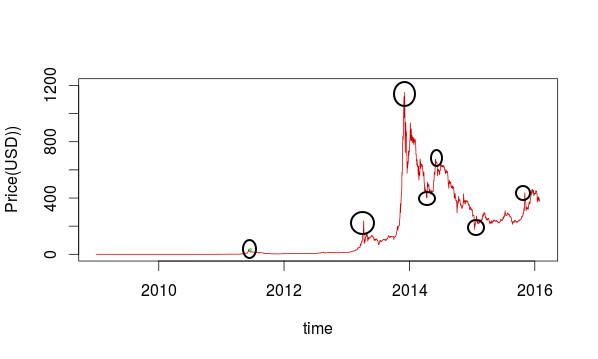
\includegraphics[width=\textwidth]{./Figures/bubble.png}
\caption{BTC Market Price (USD)}
\label{fig:bubble}
\end{center}
\end{figure}

 As the Bitcoin's complete transaction history is stored in an easily accessible and verifiable public ledger called blockchain, It is quite popular amongst economist to study bubbles. The most popular economic explanation \citep{Lo2015, Kristoufek2015} suggests that Bitcoin bubble in April, 2013, was outcome of the financial crisis in Cyprus, which triggered large numbers of people to convert euros into digital BTC. While Bouchaud  and Donier \citep{Donier2015} believe that bubbles were conditioned by the market liquidity, which triggered mismatch between the aggregate market order flow imbalance that becomes strongly negative and the prevailing liquidity on the buy side. In simple words, because of high price, buyers got too scarce to resist the pressure of a sell-off.
 
The complex, cryptic and enormous(over 60 million transactions) data-structure of blockchain had limited researchers to do in-depth transaction analysis even in computer science field. Kondor et al. \citep{Kondor2014} reconstructed the transaction network between users and analyze changes in the structure of the subgraph induced by the most active users. By using unsupervised identification of important features of the time variation of the network and Principal Component Analysis to the matrix constructed from snapshots of the network at different times, they were able to show that structural changes in the network accompany significant changes in the exchange price of bitcoins. The one fall-back about this paper is scalability, which makes it unsuitable for application having nodes greater than 10000 nodes. Other studies \citep{Kristoufek2015} uses digital behavioral traces (eg. twitter etc), wavelet coherence analysis and logistic regression to investigates bubbles, which is not a refine method considering the availability of data \citep{Ali2014}.

\section{Graph Similarity and Subgraph Matching}
\label{sec:gs}
The ultimate goal in financial market is predicting long-term asset prices, as they are so difficult to predict, Bitcoin prices are no different. The margin error with Bitcoin can be particularly brutal for extreme predictions, which usually have a lower probability of being realized. While
there has been significant research done to analyze Bitcoin transaction network, limited research has been executed to analyze the network’s influence on overall Bitcoin price. To achieve the former, one need to efficiently measures the structural change (eg. walks) of a dynamic
large-scale graph as well as the similarity between two graphs with
reference to price change. Kondor et al. \citep{Kondor2014} research was one step in the direction of basic graph similarity and subgraph matching algorithms, which is not scalable with increasing size of daily transactions \ref{fig:transactions}. 

\begin{figure}[ht]
\begin{center}
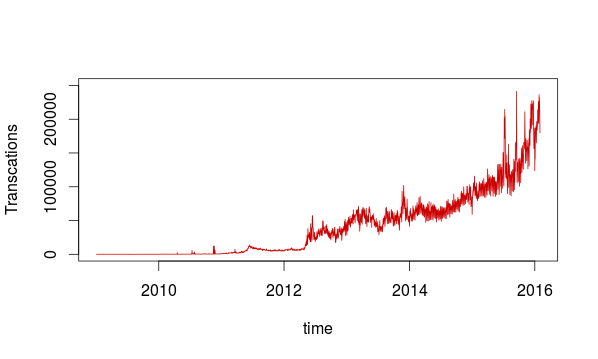
\includegraphics[width=\textwidth]{./Figures/transactions.png}
\caption{Daily Transactions}
\label{fig:transactions}
\end{center}
\end{figure}

Most of graph isomorphism algorithms and its generalizations are exponential and, thus, not applicable to the large graphs that are of interest today. The other methods  for graph similarity and graph sub-matching, like features extractions, iterative methods and tensors analysis, including some come with their drawbacks \citep{Zager2008}.

In the recent paper on graph kernels, Yanardag and Vishwanathan \citep{Yanardag2015} used "Deep Graph Kernels", a unified framework to learn latent representations of sub-structures for graphs to measure similarity. As Bitcoin transaction network graph is increasing everyday, It would be interesting to capture its structural dynamics without compromising on the graph features.

\section{Motivation}
\label{sec: motivation}

The volatile rise and fall of Bitcoin, cryptological mining, complex distributed database, blockchain and evolving network dynamics prompted me to  efficiently measures the structural change (eg. walks) of a dynamic large-scale graph as well as the similarity between two graphs with reference to price change. 

In simple words, the thesis attempts to address two important questions:  
\begin{enumerate}
\item How much is a large-scale graph (bitcoin transaction graph) transformed over time or by a significant event (bubbles)?
\item How structurally similar are two large-scale graph (bitcoin transactions graphs)?
\end{enumerate}

\section{Objective}
\label{sec: objective}

\begin{enumerate}
\item Given complex cryptic distributed blockchain, parsing it to extract transaction attributes in the form transactions graphs.
\item Given two graphs $G_1^{t_1} (n_1 , e_1 )$ and $G_2^{t_2} (n_2 , e_2)$, find an algorithm to calculate the similarity index ($0-1$) between the two graphs. This is quantitative measure of transformation over time.
\item Given a graph time series, where there are $T$ number of graphs, find approximate subgraphs belong to particular events (says bubbles -10-15\% rise/fall in BTC/USD) that occur in a subset of the $T$ graphs. 
\end{enumerate}

\section{Contribution}
\label{sec:contribution}

The decentralized paradigm of Bitcoin requires each node of the network
to retain the blockchain, which consists of all public, transparent, and permanently transactions recorded since the origin. Therefore, blockchain acts as the central point of potentially interesting information ready to be mined. But ever growing size of blockchain (60 GB as of now) makes the job difficult to parse from the raw blockchain. Adding to the same, the newer bitcoin clients indexed the full blockchain using LevelDB makes the earlier public available software obsolete. This thesis aims to develop open source blockchain parsing tools to extract agent resolved data, which can be used to extend the stucked research in bitcoin transaction dynamics. 

To understand how much a large-scale graph (bitcoin transaction graph) transformed over time or by a significant event (bubbles), we use quite novel framework for graph kernels inspired by latest advancements in natural language processing and deep learning, "deep graph propagation kernels" to have quantitative measure of transformation, which captures correlation between network structure and market price. It outperforms its best base variants in terms of capturing .
 

 
\section{Thesis Organization}

The rest of this thesis is organised as follows. In Chapter \ref{Chapter2}, 
we introduces Bitcoin, its working in detail by explaining the protocol of blockchain. Then, the data preparation staged is discussed to get the transaction network, which is used to reproduce transaction dynamics in terms of money flow, also a data validation method.  With data in hand, Chapter \ref{Chapter3} motivates to the graph isomorphism in our context, then reviews the important studies in graph isomorphism problem with advantages and disadvantages. Chapter \ref{Chapter4} starts with review of representative graph kernels in the literature. By taking conventional and sophisticated graph kernels, this chapter defines quantitative measure of transformation over time. The chapter concludes with not so smooth correspondence between network structure and exchange price in bitcoin, thus paving way for further investigation to other graph kernels. With graph kernels not giving desired results, Chapter \ref{Chapter5} propose a general framework that learns hidden representations of sub-structures used in graph kernels, inspired
by deep graph kernels. Then, the framework  is demonstrated on propagation kernels, which performs better than normal kernels. Then new graph kernel is used to calculate similarity index, which is plotted to find correlation between network structure and market price. Chapter \ref{Chapter6} concludes the thesis.

%----------------------------------------------------------------------------------------



%% Chapter 1
\chapter{Introduction} % Main chapter title

\label{Chapter1} % For referencing the chapter elsewhere, use \ref{Chapter1} 

\lhead{Chapter 1. \emph{Introduction}} % This is for the header on each page - perhaps a shortened title

%----------------------------------------------------------------------------------------
Bubbles have fascinated and baffled many canny observers of financial markets. In the language of the strict orthodoxy of the efficient market theory, bubbles are outcome of sudden changes of the fundamental valuation of assets. The empirical evidence denounce that large price jumps can be explained by news, but destabilising feedback loops of behavioural origin \citep{Donier2015}. Although plausible, a clear-cut empirical evidence for
such a scenario is still lacking, but it had created enthusiasms among research communities to understand the origin of bubbles in different commodity, Bitcoin is one of them.

Bitcoin is a digital, distributed, cryptographic currency proposed under the pseudonym Satoshi Nakamoto \citep{Nakamoto2008}. In short, It can be described as a decentralized accounting system in which accounts are associated with public keys of an asymmetric encryption scheme. To access the former account, knowledge of the corresponding private key allows account holders to create digital signatures to send and receive bitcoins (BTC).

\section{Bitcoin Bubble}
\label{sec:bitcoin_bubble}

Bitcoin started trading on Mt.Gox (its market share was over 80\% on the BTC/USD spot market), the largest online Bitcoin exchange at 5 cents. Over the next	 two	 years,	BTC exchange rose slowly, but in early April 2013, the price per BTC dropped from \$266 to around \$50 and then rose to around \$100. This major bubble was succeeded by another one on 29 Nov, 2013, when, the price of a bitcoin reached an all-time high of US\$1224.76, then dropped into the \$200-\$300 range. Metaphorically, the price rise/drop is expressed as skippyball. Once skippyball pitched high in the air, the first bounce is big, then lower, and lower, until it is flat on the ground, ready for a new throw upward. Taking market price data from Blockchain the most popular Bitcoin wallet \footnote{Market Price in USD \url{https://blockchain.info/charts/market-price}}, the bubbles can be visualized in the time series plot \ref{fig:bubble} with circles representing bubbles.

\begin{figure}[ht]
\begin{center}
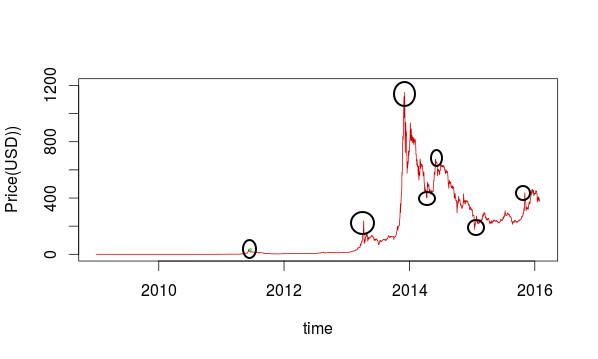
\includegraphics[width=\textwidth]{./Figures/bubble.png}
\caption{BTC Market Price (USD)}
\label{fig:bubble}
\end{center}
\end{figure}

 As the Bitcoin's complete transaction history is stored in an easily accessible and verifiable public ledger called blockchain, It is quite popular amongst economist to study bubbles. The most popular economic explanation \citep{Lo2015, Kristoufek2015} suggests that Bitcoin bubble in April, 2013, was outcome of the financial crisis in Cyprus, which triggered large numbers of people to convert euros into digital BTC. While Bouchaud  and Donier \citep{Donier2015} believe that bubbles were conditioned by the market liquidity, which triggered mismatch between the aggregate market order flow imbalance that becomes strongly negative and the prevailing liquidity on the buy side. In simple words, because of high price, buyers got too scarce to resist the pressure of a sell-off.
 
The complex, cryptic and enormous(over 60 million transactions) data-structure of blockchain had limited researchers to do in-depth transaction analysis even in computer science field. Kondor et al. \citep{Kondor2014} reconstructed the transaction network between users and analyze changes in the structure of the subgraph induced by the most active users. By using unsupervised identification of important features of the time variation of the network and Principal Component Analysis to the matrix constructed from snapshots of the network at different times, they were able to show that structural changes in the network accompany significant changes in the exchange price of bitcoins. The one fall-back about this paper is scalability, which makes it unsuitable for application having nodes greater than 10000 nodes. Other studies \citep{Kristoufek2015} uses digital behavioral traces (eg. twitter etc), wavelet coherence analysis and logistic regression to investigates bubbles, which is not a refine method considering the availability of data \citep{Ali2014}.

\section{Graph Similarity and Subgraph Matching}
\label{sec:gs}
The ultimate goal in financial market is predicting long-term asset prices, as they are so difficult to predict, Bitcoin prices are no different. The margin error with Bitcoin can be particularly brutal for extreme predictions, which usually have a lower probability of being realized. While
there has been significant research done to analyze Bitcoin transaction network, limited research has been executed to analyze the network’s influence on overall Bitcoin price. To achieve the former, one need to efficiently measures the structural change (eg. walks) of a dynamic
large-scale graph as well as the similarity between two graphs with
reference to price change. Kondor et al. \citep{Kondor2014} research was one step in the direction of basic graph similarity and subgraph matching algorithms, which is not scalable with increasing size of daily transactions \ref{fig:transactions}. 

\begin{figure}[ht]
\begin{center}
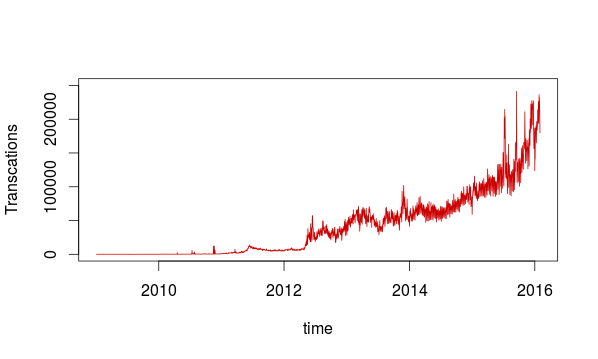
\includegraphics[width=\textwidth]{./Figures/transactions.png}
\caption{Daily Transactions}
\label{fig:transactions}
\end{center}
\end{figure}

Most of graph isomorphism algorithms and its generalizations are exponential and, thus, not applicable to the large graphs that are of interest today. The other methods  for graph similarity and graph sub-matching, like features extractions, iterative methods and tensors analysis, including some come with their drawbacks \citep{Zager2008}.

In the recent paper on graph kernels, Yanardag and Vishwanathan \citep{Yanardag2015} used "Deep Graph Kernels", a unified framework to learn latent representations of sub-structures for graphs to measure similarity. As Bitcoin transaction network graph is increasing everyday, It would be interesting to capture its structural dynamics without compromising on the graph features.

\section{Motivation}
\label{sec: motivation}

The volatile rise and fall of Bitcoin, cryptological mining, complex distributed database, blockchain and evolving network dynamics prompted me to  efficiently measures the structural change (eg. walks) of a dynamic large-scale graph as well as the similarity between two graphs with reference to price change. 

In simple words, the thesis attempts to address two important questions:  
\begin{enumerate}
\item How much is a large-scale graph (bitcoin transaction graph) transformed over time or by a significant event (bubbles)?
\item How structurally similar are two large-scale graph (bitcoin transactions graphs)?
\end{enumerate}

\section{Objective}
\label{sec: objective}

\begin{enumerate}
\item Given complex cryptic distributed blockchain, parsing it to extract transaction attributes in the form transactions graphs.
\item Given two graphs $G_1^{t_1} (n_1 , e_1 )$ and $G_2^{t_2} (n_2 , e_2)$, find an algorithm to calculate the similarity index ($0-1$) between the two graphs. This is quantitative measure of transformation over time.
\item Given a graph time series, where there are $T$ number of graphs, find approximate subgraphs belong to particular events (says bubbles -10-15\% rise/fall in BTC/USD) that occur in a subset of the $T$ graphs. 
\end{enumerate}

\section{Contribution}
\label{sec:contribution}

The decentralized paradigm of Bitcoin requires each node of the network
to retain the blockchain, which consists of all public, transparent, and permanently transactions recorded since the origin. Therefore, blockchain acts as the central point of potentially interesting information ready to be mined. But ever growing size of blockchain (60 GB as of now) makes the job difficult to parse from the raw blockchain. Adding to the same, the newer bitcoin clients indexed the full blockchain using LevelDB makes the earlier public available software obsolete. This thesis aims to develop open source blockchain parsing tools to extract agent resolved data, which can be used to extend the stucked research in bitcoin transaction dynamics. 

To understand how much a large-scale graph (bitcoin transaction graph) transformed over time or by a significant event (bubbles), we use quite novel framework for graph kernels inspired by latest advancements in natural language processing and deep learning, "deep graph propagation kernels" to have quantitative measure of transformation, which captures correlation between network structure and market price. It outperforms its best base variants in terms of capturing .
 

 
\section{Thesis Organization}

The rest of this thesis is organised as follows. In Chapter \ref{Chapter2}, 
we introduces Bitcoin, its working in detail by explaining the protocol of blockchain. Then, the data preparation staged is discussed to get the transaction network, which is used to reproduce transaction dynamics in terms of money flow, also a data validation method.  With data in hand, Chapter \ref{Chapter3} motivates to the graph isomorphism in our context, then reviews the important studies in graph isomorphism problem with advantages and disadvantages. Chapter \ref{Chapter4} starts with review of representative graph kernels in the literature. By taking conventional and sophisticated graph kernels, this chapter defines quantitative measure of transformation over time. The chapter concludes with not so smooth correspondence between network structure and exchange price in bitcoin, thus paving way for further investigation to other graph kernels. With graph kernels not giving desired results, Chapter \ref{Chapter5} propose a general framework that learns hidden representations of sub-structures used in graph kernels, inspired
by deep graph kernels. Then, the framework  is demonstrated on propagation kernels, which performs better than normal kernels. Then new graph kernel is used to calculate similarity index, which is plotted to find correlation between network structure and market price. Chapter \ref{Chapter6} concludes the thesis.

%----------------------------------------------------------------------------------------


 
%----------------------------------------------------------------------------------------
%	THESIS CONTENT - CHAPTER2
%----------------------------------------------------------------------------------------

%\mainmatter % Begin numeric (1,2,3...) page numbering

\pagestyle{fancy} % Return the page headers back to the "fancy" style

% Include the chapters of the thesis as separate files from the Chapters folder
% Uncomment the lines as you write the chapters

% Chapter 2
\chapter{Bitcoin Transaction Dynamics } % Main chapter title

\label{Chapter2} % For referencing the chapter elsewhere, use \ref{Chapter2} 

\lhead{Chapter 2. \emph{Bitcoin Transaction Dynamics}} % This is for the header on each page - perhaps a shortened title

%----------------------------------------------------------------------------------------
\section{Introduction}

Bitcoin is a decentralized peer to peer electronic payment system in which transactions are performed with no central authority or banks to authorize it. The Bitcoin transactions management and its issuance is carried out collectively by the network. The first Bitcoin specification and proof of concept was published by Satoshi Nakamoto \citep{Nakamoto2008} in 2009 cryptographic mailing list. Bitcoin can also be seen as the most prominent triple entry bookkeeping system in existence. Since then, the community has grown exponentially with many developers working on Bitcoin.


\section{Bitcoin}
\label{sec:bitcoin}
Bitcoin payments use public keys encryption, where, payers and payees are identified by hashed public keys of their Bitcoin wallets. The public keys are generated by ECDSA (Elliptic Curve Digital Signature Algorithm), based on calculations of elliptical curves over finite space. Suppose, Alice sends "$x$" coins to Bob, then an unencrypted transaction attaching Bob's public key is broadcast over the Bitcoin network using her private key. The signature on transaction verifies all users for its authenticity (current owner of coin) by looking at complete history of transactions, called {\it blockchain}. It is essential element in bitcoin architecture, which verifies the legitimacy of ability (sufficient bitcoins) of Alice paying Bob.

\subsection{Blockchain}


The complete record of transactions is in a coded form in a data structure called {\it blockchain}, which is a sequence of records called {\it blocks}. Each block contains a group of transactions that have been sent since the previous block, with integrity check all the way back to the first one, the genesis block.

Any users enter the Bitcoin system by trading non-digital currencies at Bitcoin market exchange, or by mining coins, which involves solving a cryptographically hard problem for which he/she is suitably rewarded a fixed number of Bitcoins  and transactions is validated on the network. The working of mining, core to {\it blockchain}, is mathematically explained better by Johannes et al. \cite{Johannes2015}. The network of peers, called miners, are the agents using computers, who actually add the blocks to the blockchain. Taking example of Alice sending "$x$" coins to Bob from section \ref{sec:bitcoin} by broadcasting over network. The miners receives copies of all transactions as they are generated, including Alice's copy. The blockchain is examined to investigate the history of the bitcoins involved in each transaction. If the proposed transaction from the Alice has sufficient bitcoin credit, then it is accepted for incorporation into the block that the miner is currently working on. 


Identifying each transaction with a double SHA-256 hash, the transactions is gathered together. Then by using miners hashes,together with the hash that is at the current head of the blockchain, as inputs to the cryptographic problem is solved by miners, with rewards of 25 bitcoins in 10 minutes \cite{Johannes2015}. At first, miner~$M$ computes a block hash~$h$ over a unique ordering of the hashes of all the transactions that it is intending to incorporate into its next block $B$.  Then, input of the block solution $s_{i-1}$ is taken at the head of its current version of the {\it blockchain}. If we concatenate the strings by the symbol $+$, the cryptographic problem that $M$ has to solve is: compute a SHA-256 hash
%
\begin{equation} \label{eq:2.1}
s_i = (n + h + s_{i-1}),
\end{equation}
%
such that $s_i$ has at least a specified number~$x$ of leading zeros where $x \sim 64$. 

Once mined, the new block is communicated by broadcasting newly-discovered
blocks via a peer-to-peer network to add the new block at blockchain at each peer using blockchain protocol rules. This makes blockchain as a public ledger, recording  every Bitcoin payment ever made. The simplified version of the whole process is represented in below illustration \ref{fig:blockchain}.

\begin{figure}[ht]
\begin{center}
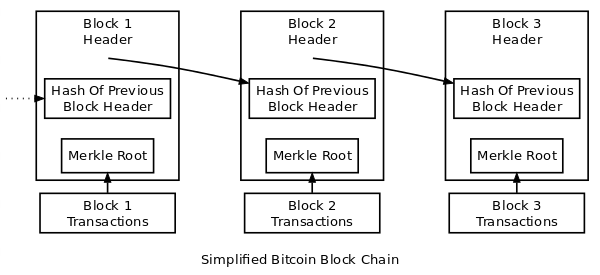
\includegraphics[width=0.8\textwidth]{./Figures/blockchain.png}
\caption{Simple Blockchain \citep{Blockchain2016}}
\label{fig:blockchain}
\end{center}
\end{figure}
The transaction data part of a block consists of one or more new transactions. While the merkel root of the merkle tree contains  hashed copies of each transaction, and the hashes are then paired, hashed, paired again, and hashed again until a single hash remains. The chaining of blocks together and storing the hash of the previous block’s header ensures a transaction cannot be modified without modifying the block that records it and all following blocks. The same goes with the transaction, which are also chained together. A single transaction can create multiple outputs, which  are tied to transaction identifiers (TXIDs), the hashes of signed transactions. Also, the outputs of all transactions included in the block chain can be categorized as either Unspent Transaction Outputs (UTXOs) or spent transaction outputs \ref{fig:block_t}. The first one of these transactions called a generation transaction, which should collect and spend the block reward (comprised of a block subsidy and any transaction fees paid by transactions included in this block). All these transactions are encoded into blocks in binary rawtransaction format, making it difficult for researchers to extract in simple relational database format, to get transaction graph.

\begin{figure}[ht]
\begin{center}
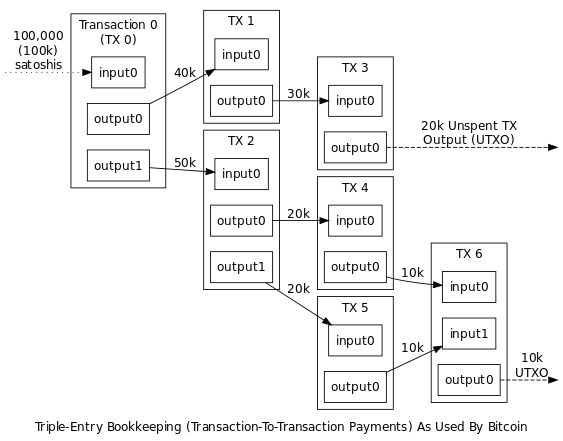
\includegraphics[width=0.8\textwidth]{./Figures/block_t.png}
\caption{Blockchain Transaction \citep{Blockchain2016}}
\label{fig:block_t}
\end{center}
\end{figure}

\section{Related Work}
The possibility to analyze agent resolved transactions in any market is limited by the scarcity of available data, as this kind of information is usually considered highly sensitive. But with the publicly available blockchain at every machine allows researchers to reconstruct the network of transactions and extract the time and amount of each payment. There are many research studies that concerns bitcoin transaction network using network analysis, machine learning and statistical physics techniques.

Parsing four (2009-2013) years data from bitcoin's  blockchain, Kondor et al. \citep{Csabai2014}  analyze the structure of the transaction network by measuring network characteristics over time, such as the degree distribution, degree correlations, clustering and money movement. Using the same data, they in their different paper \citep{Kondor2014} analyze changes in the structure of the subgraph induced by the most active users. They were  able to show find correlation between structural changes in the network and exchange price of bitcoins. But with exponential increase in the number of transaction over years, they method seems obsolete , as it is difficult to scale with their endorsed methods.

Reid and Harrigan \citep{Reid2013} linked addresses belonging to the same entity using external information. The using techniques such as context discovery and flow analysis, they investigate an alleged theft of Bitcoins. By running the Union-Find algorithm, Ron and Samir \citep{Ron2013}  associated the 3,120,948 addresses with 1,851,544 different entities to understand behaviour of users. Spagnuolo \citep{Spagnuolo2013} released open source project Bitiodine, which was able to cluster addresses and classify them using a dataset partially obtained in an automatic fashion, using scrapers for major web sources of bitcoin addresses. On the similar line, other paper \citep{Fleder2015} investigates bitcoin transaction-graph-annotation, which is capable of tracing and clustering user activity.

Most of the  previous research employed data collected from old Bitcoin- client Bitcoin 0.8 later, the newer bitcoin clients indexed the full blockchain using LevelDB instead making the publicly available bitcointools obsolete. Adding to the same, the nearing 300,000 transactions/day in 2015 gives really hard time to earlier algorithms to scale, thus motivating us to develop new techniques to parsing data from blockchain, reconstructing network and doing analysis.

\section{Data}
\label{data}
The blockchain is a transaction database of the Bitcoin.  Once Bitcoin core is setup at local machine, blockchain is automatically downloaded. Every full node participating in the Bitcoin network has the same copy. As of now there is more than 60 GB of Bitcoin blockchain dataset, which makes it difficult to parse the raw blockchain data. Most of the previous studies \citep{Ron2013} employed a forked version of bitcointools \footnote{\url{https://github.com/gavinandresen/bitcointools}}, but from the bitcoin clients 0.8 version, it indexed the full blockchain using LevelDB instead making the publicly available bitcointools obsolete. Other well know open source blockchain parser like blockparser \footnote{\url {https://github.com/znort987/blockparser}}, BitIodine \citep{Spagnuolo2013} etc are almost undocumented projects, where some appear to not even work. A paper \citep{Fleder2015} led me to BitcoinArmory project, which requires a dozen of manual interventions to get installed, but still doesn’t work.

We then started to look for ready-made SQL database, which pointed to BitcoinABe. This python based library reads the Bitcoin block file, transforms and loads the data into a SQL database \ref{fig:SQL}. But, Its takes more than two weeks to dump the data, which was not feasible option. We downloaded postgres database dumps of the bitcoin-ruby-blockchain database generated by webbtc \footnote{\url{http://dumps.webbtc.com/bitcoin/}}. Then, with slight modification to open repository BitIodine \citep{Spagnuolo2013} code, we parsed through the blockchain, and wrote wrapper classes that extracted the relevant information required to construct the transaction graph. The market price data was scarped from website \url {https://blockchain.info/} to plot graphs in R.

\section{Bitcoin Transaction Network}

Before getting the transaction network, we first define our graph, which acts as input to further mathematical application.

\begin{definition}
We consider weighted labelled graph. That is, a
graph $G=(V,E,\ell)$ is represented by a set of $|V|=n$ vertices, a
set of edges $E$ specified by a weighted adjacency matrix $A \in
\bb{R}^{n \times n}$, and a label function $\ell\colon V \rightarrow
\cm{L}$ with $\cm{L} = \left( [k], \R^D \right)$, where $k$ is the
number of available node labels and $D$ is the dimension of the
continuous attributes.  Given $V = \{v_1,v_2,...,v_n\}$, \emph{node
  labels} $\ell(v_i)$ are represented by nominal values and
\emph{attributes} $\mathbf{x}_i \in \bb R^D$ are represented by
continuous vectors. In a transaction graph, addresses are nodes, transactions are edges and weight is BTC.
\label{def:graph}
\end{definition}

With the overall transactions records parsed from the blockchain in human readable form, we construct a a weighted directed transaction graph that gives an intuition towards the flow of Bitcoins from one key to the other,the directed edge represents a particular transaction from a source address to a target address and weight represents the value of the transactions. For our experiments, we constructed graphs for more than two years (March, 2013 to December, 2015) to capture major bubble in Bitcoin history. Figure \ref{fig:dt} represent daily transaction graph for a typical day on April 8, 2013.

\begin{figure}[ht]
\begin{center}
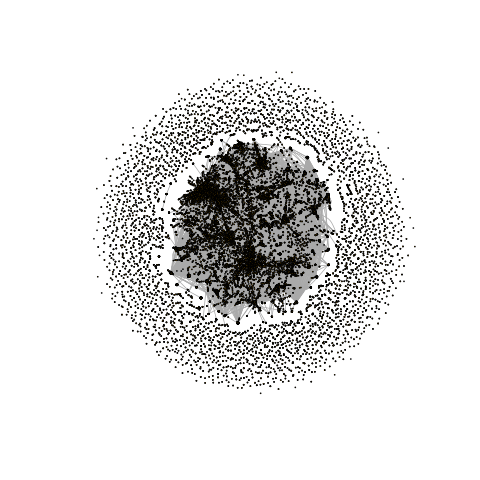
\includegraphics[width=\textwidth]{./Figures/dt.png}
\caption{ Daily transaction graph for a typical day (April 8, 2013)}
\label{fig:dt}
\end{center}
\end{figure}

\section{Transaction Dynamics}
The validation of the data parsed from our tool is then checked by
reproducing the ”Mathew Effect” phenomenon from the seminal work of Kondor et al. \citep{Csabai2014} paper’s using their original matlab code, but with our own data. The authors of the above papers are curator of whole blockchain up to 2014.10.19. (326,027 blocks), which is benchmark in quality. The similar figure confirms the high quality of our data.

To capture the transaction  dynamics in the bitcoin, we analyze the dynamics of money flow on the transaction network, as discussed in the paper \citep{Csabai2014}. We try to support popular hypothesis in economics having roots in preferential attachment, called Matthew effect or the "rich get richer phenomenon". It states that the growth of the wealth of each individual is proportional to the wealth of that individual \citep{Csabai2014}.

We assume that the number of bitcoins associated with node $n$ at time $t$ is given by $b_{n}(t)$. The difference between the balance of each
address at the end and at the start of each month is calculated. Then the difference in function of the starting balances is plotted in figure \ref{fig:dynamics}. The  positive correlation between balance and the average growth indicates the "rich get richer" phenomenon in bitcoin.

\begin{figure}[ht]
\begin{center}
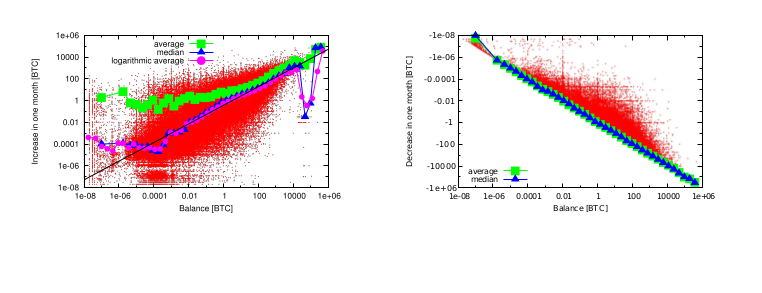
\includegraphics[width= \textwidth]{./Figures/dynamics.png}
\caption{ Matthew Effect}
\label{fig:dynamics}
\end{center}
\end{figure}

The figure \ref{fig:dynamics} is reproduced from Kondor's paper \citep{Csabai2014}, using our own data where Increase (left) and decrease (right) of node balances in one month windows as a function of their balance at the beginning of each month is represented. The representation in the picture follow the following colors: the raw data (red), the average (green), median (blue) and logarithmic average (magenta). The later three are calculated for logarithmically sized bins. The power-law fit for the double logarithmic data is represented by black line.

\subsection{Silk Road Arrest}

The Silk Road, under the alias of “Dread Pirate Roberts” (DPR) was known as an anonymous marketplace, a Black Market operated as a hidden service only accessible through Tor, where people who use bitcoins were able to buy and sell drugs, art, weapons etc. anonymously, without the risk of being tracked. It was founded by Ross William Ulbricht in February in 2011, but in October 2013 FBI closed the Silk Road and arrested Ulbricht. The FBI  seized approximately 173,600 BTC in two phase. At the first go 29,600 BTC held in a so called hot wallet were seized and an additional 144,000 BTC were seized using two addresses \footnote{1F1tAaz5x1HUXrCNLbtMDqcw6o5GNn4xqX, 1FfmbHfnpaZjKFvyi1okTjJJusN455paPH} controlled by the FBI. 

We illustrates the event using transaction network \ref{fig:silk} realised in gephi. Each vertex represents a user, where address is mapped to the user. Each directed edge between a source and a target represents a flow of Bitcoins from a public-key belonging to the user corresponding to the source to a public-key belonging to the user corresponding to the target. 

\begin{figure}[ht]
\begin{center}
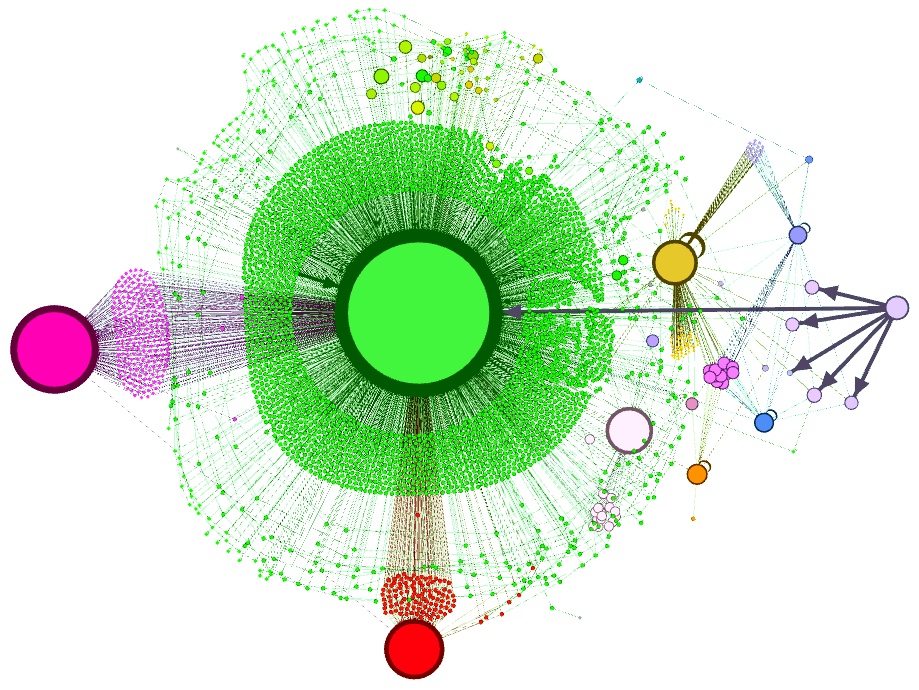
\includegraphics[width=0.7\textwidth]{./Figures/silk.png}
\caption{ Silk Road Arrest}
\label{fig:silk}
\end{center}
\end{figure}

Although in this scenario involves manual investigation by web scraping , it would have been difficult to find significant links manually, given the millions of nodes involved.

\section{Summary}
This chapter introduces Bitcoin, its working detail by explaining the protocol of blockchain, which contains all the history of transactions in the bitcoin. With enough knowledge about working of bitcoin, the related work in bitcoin transaction network is the discussed with the pros and cons. The data preparation staged is discussed to get the transaction network, an input to our mathematical model in coming chapters. The case study of silk road arrest is illustrated with the transaction graph. Transaction dynamics is reproduced from know studies to validate the parsed data, concludes the chapter.
%% Chapter 2
\chapter{Bitcoin Transaction Dynamics } % Main chapter title

\label{Chapter2} % For referencing the chapter elsewhere, use \ref{Chapter2} 

\lhead{Chapter 2. \emph{Bitcoin Transaction Dynamics}} % This is for the header on each page - perhaps a shortened title

%----------------------------------------------------------------------------------------
\section{Introduction}

Bitcoin is a decentralized peer to peer electronic payment system in which transactions are performed with no central authority or banks to authorize it. The Bitcoin transactions management and its issuance is carried out collectively by the network. The first Bitcoin specification and proof of concept was published by Satoshi Nakamoto \citep{Nakamoto2008} in 2009 cryptographic mailing list. Bitcoin can also be seen as the most prominent triple entry bookkeeping system in existence. Since then, the community has grown exponentially with many developers working on Bitcoin.


\section{Bitcoin}
\label{sec:bitcoin}
Bitcoin payments use public keys encryption, where, payers and payees are identified by hashed public keys of their Bitcoin wallets. The public keys are generated by ECDSA (Elliptic Curve Digital Signature Algorithm), based on calculations of elliptical curves over finite space. Suppose, Alice sends "$x$" coins to Bob, then an unencrypted transaction attaching Bob's public key is broadcast over the Bitcoin network using her private key. The signature on transaction verifies all users for its authenticity (current owner of coin) by looking at complete history of transactions, called {\it blockchain}. It is essential element in bitcoin architecture, which verifies the legitimacy of ability (sufficient bitcoins) of Alice paying Bob.

\subsection{Blockchain}


The complete record of transactions is in a coded form in a data structure called {\it blockchain}, which is a sequence of records called {\it blocks}. Each block contains a group of transactions that have been sent since the previous block, with integrity check all the way back to the first one, the genesis block.

Any users enter the Bitcoin system by trading non-digital currencies at Bitcoin market exchange, or by mining coins, which involves solving a cryptographically hard problem for which he/she is suitably rewarded a fixed number of Bitcoins  and transactions is validated on the network. The working of mining, core to {\it blockchain}, is mathematically explained better by Johannes et al. \cite{Johannes2015}. The network of peers, called miners, are the agents using computers, who actually add the blocks to the blockchain. Taking example of Alice sending "$x$" coins to Bob from section \ref{sec:bitcoin} by broadcasting over network. The miners receives copies of all transactions as they are generated, including Alice's copy. The blockchain is examined to investigate the history of the bitcoins involved in each transaction. If the proposed transaction from the Alice has sufficient bitcoin credit, then it is accepted for incorporation into the block that the miner is currently working on. 


Identifying each transaction with a double SHA-256 hash, the transactions is gathered together. Then by using miners hashes,together with the hash that is at the current head of the blockchain, as inputs to the cryptographic problem is solved by miners, with rewards of 25 bitcoins in 10 minutes \cite{Johannes2015}. At first, miner~$M$ computes a block hash~$h$ over a unique ordering of the hashes of all the transactions that it is intending to incorporate into its next block $B$.  Then, input of the block solution $s_{i-1}$ is taken at the head of its current version of the {\it blockchain}. If we concatenate the strings by the symbol $+$, the cryptographic problem that $M$ has to solve is: compute a SHA-256 hash
%
\begin{equation} \label{eq:2.1}
s_i = (n + h + s_{i-1}),
\end{equation}
%
such that $s_i$ has at least a specified number~$x$ of leading zeros where $x \sim 64$. 

Once mined, the new block is communicated by broadcasting newly-discovered
blocks via a peer-to-peer network to add the new block at blockchain at each peer using blockchain protocol rules. This makes blockchain as a public ledger, recording  every Bitcoin payment ever made. The simplified version of the whole process is represented in below illustration \ref{fig:blockchain}.

\begin{figure}[ht]
\begin{center}
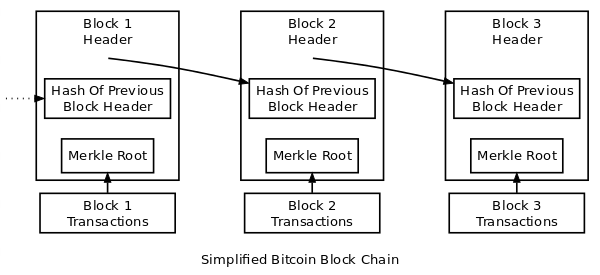
\includegraphics[width=0.8\textwidth]{./Figures/blockchain.png}
\caption{Simple Blockchain \citep{Blockchain2016}}
\label{fig:blockchain}
\end{center}
\end{figure}
The transaction data part of a block consists of one or more new transactions. While the merkel root of the merkle tree contains  hashed copies of each transaction, and the hashes are then paired, hashed, paired again, and hashed again until a single hash remains. The chaining of blocks together and storing the hash of the previous block’s header ensures a transaction cannot be modified without modifying the block that records it and all following blocks. The same goes with the transaction, which are also chained together. A single transaction can create multiple outputs, which  are tied to transaction identifiers (TXIDs), the hashes of signed transactions. Also, the outputs of all transactions included in the block chain can be categorized as either Unspent Transaction Outputs (UTXOs) or spent transaction outputs \ref{fig:block_t}. The first one of these transactions called a generation transaction, which should collect and spend the block reward (comprised of a block subsidy and any transaction fees paid by transactions included in this block). All these transactions are encoded into blocks in binary rawtransaction format, making it difficult for researchers to extract in simple relational database format, to get transaction graph.

\begin{figure}[ht]
\begin{center}
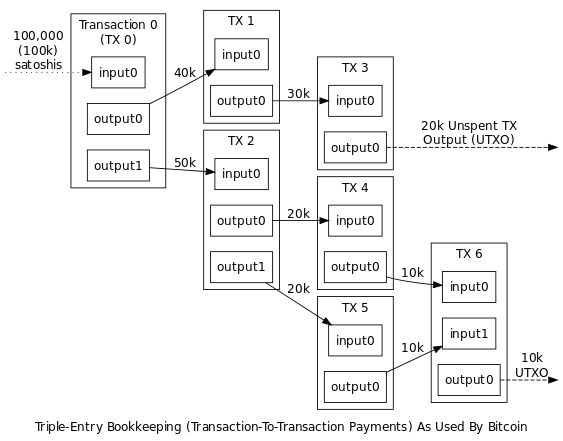
\includegraphics[width=0.8\textwidth]{./Figures/block_t.png}
\caption{Blockchain Transaction \citep{Blockchain2016}}
\label{fig:block_t}
\end{center}
\end{figure}

\section{Related Work}
The possibility to analyze agent resolved transactions in any market is limited by the scarcity of available data, as this kind of information is usually considered highly sensitive. But with the publicly available blockchain at every machine allows researchers to reconstruct the network of transactions and extract the time and amount of each payment. There are many research studies that concerns bitcoin transaction network using network analysis, machine learning and statistical physics techniques.

Parsing four (2009-2013) years data from bitcoin's  blockchain, Kondor et al. \citep{Csabai2014}  analyze the structure of the transaction network by measuring network characteristics over time, such as the degree distribution, degree correlations, clustering and money movement. Using the same data, they in their different paper \citep{Kondor2014} analyze changes in the structure of the subgraph induced by the most active users. They were  able to show find correlation between structural changes in the network and exchange price of bitcoins. But with exponential increase in the number of transaction over years, they method seems obsolete , as it is difficult to scale with their endorsed methods.

Reid and Harrigan \citep{Reid2013} linked addresses belonging to the same entity using external information. The using techniques such as context discovery and flow analysis, they investigate an alleged theft of Bitcoins. By running the Union-Find algorithm, Ron and Samir \citep{Ron2013}  associated the 3,120,948 addresses with 1,851,544 different entities to understand behaviour of users. Spagnuolo \citep{Spagnuolo2013} released open source project Bitiodine, which was able to cluster addresses and classify them using a dataset partially obtained in an automatic fashion, using scrapers for major web sources of bitcoin addresses. On the similar line, other paper \citep{Fleder2015} investigates bitcoin transaction-graph-annotation, which is capable of tracing and clustering user activity.

Most of the  previous research employed data collected from old Bitcoin- client Bitcoin 0.8 later, the newer bitcoin clients indexed the full blockchain using LevelDB instead making the publicly available bitcointools obsolete. Adding to the same, the nearing 300,000 transactions/day in 2015 gives really hard time to earlier algorithms to scale, thus motivating us to develop new techniques to parsing data from blockchain, reconstructing network and doing analysis.

\section{Data}
\label{data}
The blockchain is a transaction database of the Bitcoin.  Once Bitcoin core is setup at local machine, blockchain is automatically downloaded. Every full node participating in the Bitcoin network has the same copy. As of now there is more than 60 GB of Bitcoin blockchain dataset, which makes it difficult to parse the raw blockchain data. Most of the previous studies \citep{Ron2013} employed a forked version of bitcointools \footnote{\url{https://github.com/gavinandresen/bitcointools}}, but from the bitcoin clients 0.8 version, it indexed the full blockchain using LevelDB instead making the publicly available bitcointools obsolete. Other well know open source blockchain parser like blockparser \footnote{\url {https://github.com/znort987/blockparser}}, BitIodine \citep{Spagnuolo2013} etc are almost undocumented projects, where some appear to not even work. A paper \citep{Fleder2015} led me to BitcoinArmory project, which requires a dozen of manual interventions to get installed, but still doesn’t work.

We then started to look for ready-made SQL database, which pointed to BitcoinABe. This python based library reads the Bitcoin block file, transforms and loads the data into a SQL database \ref{fig:SQL}. But, Its takes more than two weeks to dump the data, which was not feasible option. We downloaded postgres database dumps of the bitcoin-ruby-blockchain database generated by webbtc \footnote{\url{http://dumps.webbtc.com/bitcoin/}}. Then, with slight modification to open repository BitIodine \citep{Spagnuolo2013} code, we parsed through the blockchain, and wrote wrapper classes that extracted the relevant information required to construct the transaction graph. The market price data was scarped from website \url {https://blockchain.info/} to plot graphs in R.

\section{Bitcoin Transaction Network}

Before getting the transaction network, we first define our graph, which acts as input to further mathematical application.

\begin{definition}
We consider weighted labelled graph. That is, a
graph $G=(V,E,\ell)$ is represented by a set of $|V|=n$ vertices, a
set of edges $E$ specified by a weighted adjacency matrix $A \in
\bb{R}^{n \times n}$, and a label function $\ell\colon V \rightarrow
\cm{L}$ with $\cm{L} = \left( [k], \R^D \right)$, where $k$ is the
number of available node labels and $D$ is the dimension of the
continuous attributes.  Given $V = \{v_1,v_2,...,v_n\}$, \emph{node
  labels} $\ell(v_i)$ are represented by nominal values and
\emph{attributes} $\mathbf{x}_i \in \bb R^D$ are represented by
continuous vectors. In a transaction graph, addresses are nodes, transactions are edges and weight is BTC.
\label{def:graph}
\end{definition}

With the overall transactions records parsed from the blockchain in human readable form, we construct a a weighted directed transaction graph that gives an intuition towards the flow of Bitcoins from one key to the other,the directed edge represents a particular transaction from a source address to a target address and weight represents the value of the transactions. For our experiments, we constructed graphs for more than two years (March, 2013 to December, 2015) to capture major bubble in Bitcoin history. Figure \ref{fig:dt} represent daily transaction graph for a typical day on April 8, 2013.

\begin{figure}[ht]
\begin{center}
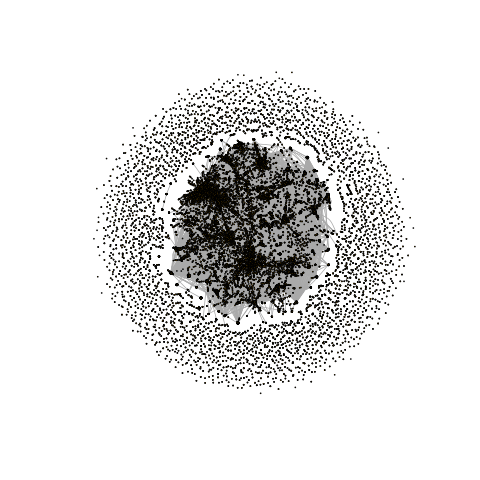
\includegraphics[width=\textwidth]{./Figures/dt.png}
\caption{ Daily transaction graph for a typical day (April 8, 2013)}
\label{fig:dt}
\end{center}
\end{figure}

\section{Transaction Dynamics}
The validation of the data parsed from our tool is then checked by
reproducing the ”Mathew Effect” phenomenon from the seminal work of Kondor et al. \citep{Csabai2014} paper’s using their original matlab code, but with our own data. The authors of the above papers are curator of whole blockchain up to 2014.10.19. (326,027 blocks), which is benchmark in quality. The similar figure confirms the high quality of our data.

To capture the transaction  dynamics in the bitcoin, we analyze the dynamics of money flow on the transaction network, as discussed in the paper \citep{Csabai2014}. We try to support popular hypothesis in economics having roots in preferential attachment, called Matthew effect or the "rich get richer phenomenon". It states that the growth of the wealth of each individual is proportional to the wealth of that individual \citep{Csabai2014}.

We assume that the number of bitcoins associated with node $n$ at time $t$ is given by $b_{n}(t)$. The difference between the balance of each
address at the end and at the start of each month is calculated. Then the difference in function of the starting balances is plotted in figure \ref{fig:dynamics}. The  positive correlation between balance and the average growth indicates the "rich get richer" phenomenon in bitcoin.

\begin{figure}[ht]
\begin{center}
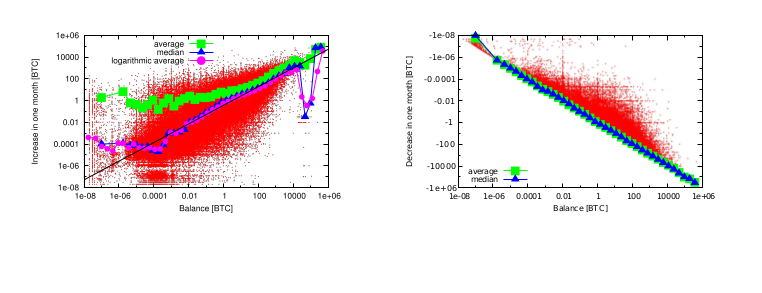
\includegraphics[width= \textwidth]{./Figures/dynamics.png}
\caption{ Matthew Effect}
\label{fig:dynamics}
\end{center}
\end{figure}

The figure \ref{fig:dynamics} is reproduced from Kondor's paper \citep{Csabai2014}, using our own data where Increase (left) and decrease (right) of node balances in one month windows as a function of their balance at the beginning of each month is represented. The representation in the picture follow the following colors: the raw data (red), the average (green), median (blue) and logarithmic average (magenta). The later three are calculated for logarithmically sized bins. The power-law fit for the double logarithmic data is represented by black line.

\subsection{Silk Road Arrest}

The Silk Road, under the alias of “Dread Pirate Roberts” (DPR) was known as an anonymous marketplace, a Black Market operated as a hidden service only accessible through Tor, where people who use bitcoins were able to buy and sell drugs, art, weapons etc. anonymously, without the risk of being tracked. It was founded by Ross William Ulbricht in February in 2011, but in October 2013 FBI closed the Silk Road and arrested Ulbricht. The FBI  seized approximately 173,600 BTC in two phase. At the first go 29,600 BTC held in a so called hot wallet were seized and an additional 144,000 BTC were seized using two addresses \footnote{1F1tAaz5x1HUXrCNLbtMDqcw6o5GNn4xqX, 1FfmbHfnpaZjKFvyi1okTjJJusN455paPH} controlled by the FBI. 

We illustrates the event using transaction network \ref{fig:silk} realised in gephi. Each vertex represents a user, where address is mapped to the user. Each directed edge between a source and a target represents a flow of Bitcoins from a public-key belonging to the user corresponding to the source to a public-key belonging to the user corresponding to the target. 

\begin{figure}[ht]
\begin{center}
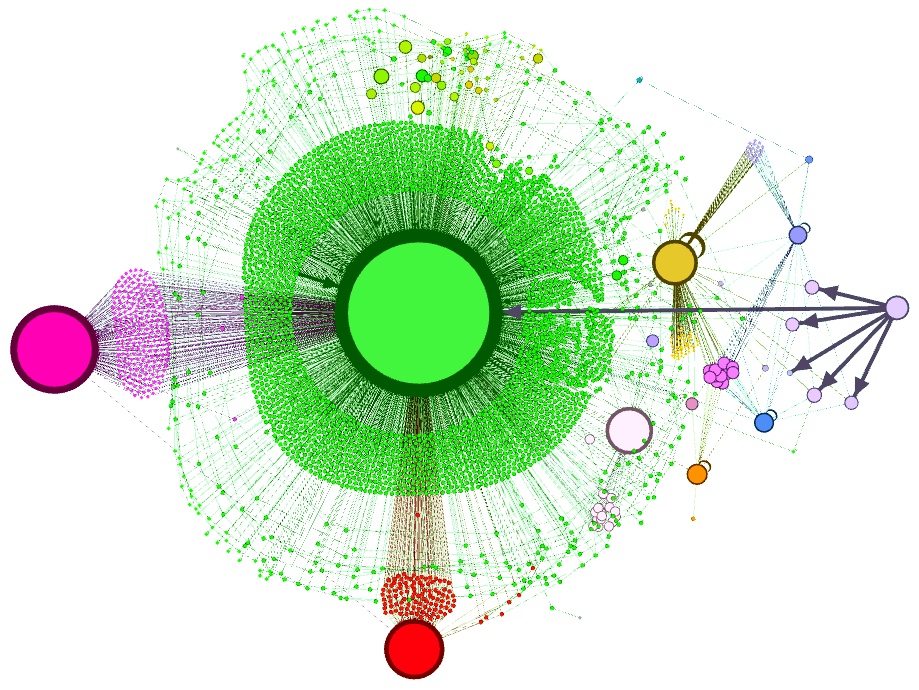
\includegraphics[width=0.7\textwidth]{./Figures/silk.png}
\caption{ Silk Road Arrest}
\label{fig:silk}
\end{center}
\end{figure}

Although in this scenario involves manual investigation by web scraping , it would have been difficult to find significant links manually, given the millions of nodes involved.

\section{Summary}
This chapter introduces Bitcoin, its working detail by explaining the protocol of blockchain, which contains all the history of transactions in the bitcoin. With enough knowledge about working of bitcoin, the related work in bitcoin transaction network is the discussed with the pros and cons. The data preparation staged is discussed to get the transaction network, an input to our mathematical model in coming chapters. The case study of silk road arrest is illustrated with the transaction graph. Transaction dynamics is reproduced from know studies to validate the parsed data, concludes the chapter. 
%----------------------------------------------------------------------------------------
%	THESIS CONTENT - CHAPTER3
%----------------------------------------------------------------------------------------

%\mainmatter % Begin numeric (1,2,3...) page numbering

\pagestyle{fancy} % Return the page headers back to the "fancy" style

% Include the chapters of the thesis as separate files from the Chapters folder
% Uncomment the lines as you write the chapters

% Chapter 3
\chapter{Graph Isomorphism} % Main chapter title

\label{Chapter3} % For referencing the chapter elsewhere, use \ref{Chapter1} 

\lhead{Chapter3. \emph{Graph Isomorphism}} % This is for the header on each page - perhaps a shortened title

%----------------------------------------------------------------------------------------
The dramatic proliferation of sophisticated networks has resulted in a growing need for supporting effective analysis and measurement of large-scale graphs whose contents change dynamically over time or after
an important event. The availability of large scale bitcoin's transactions allows us to have better understanding of the phenomena, modelled using underlying system of interacting agents. In short, It drives our research in direction to measures the structural change of a dynamic large-scale graph as well as the similarity between two graphs. At the core of above problem definition lies a common and critical graph isomorphism questions: By how much is a graph transformed over time or by a significant event? or how structurally similar are graphs?

\section{Problem Definition}

\subsection{Problem: Graph Similarity}

Two graph $G_{1} = (V_{1},E_{1},\ell_{1})$ and $G_{2} = (V_{2},E_{2},\ell_{2})$ are isomorphic, denoted by $G_{1} \cong G_{2}$, if there is a structure-preserving bijection $f \colon V_{1} \rightarrow V_{2}$ so that if $ \{ e_{1}, e_{2} \} \in E_{1}$ then $ \{ f(e_{1}), f(e_{2}) \} \in E_{2}$.  where $V$ is the set of nodes and $E$ is the set of edges in graph $G$. Weighted adjacency matrices $A \in \mathbb{R}^{n_i \times n_i}$ represents and the label function~$\ell$ endows nodes with label and attribute information.

\subsection{Solution: Similarity Index}

Similarity Index, intuitively signifying the structural similarity between two given graphs is defined as $SI (G_{1}, G_{2})$,  $ 0 \leq SI(G_{1}, G_{2}) \leq 1 $. Where,  $SI (G_{1}, G_{2}) = 0 $ indicates that two graphs are structurally complementary and  $SI (G_{1}, G_{2}) = 1$ means two graphs are completely identical.



\section{Literature Review}
Long in the purview of researchers, graph isomorphism is a well-studied problem in literature. Besides its practical importance, the graph isomorphism problem is a curiosity in computational complexity theory as it is one of a very small number of problems belonging to NP neither known to be solvable in polynomial time nor NP-complete. The classic open problem in the algorithmic theory of random graphs for decades was recently solved by Babai \citep{Babai2016}. He showed that it can be solved in in quasipolynomial time. Unfortunately, an algorithm has not yet been created to test such algorithms, thus, it will have to be vetted by other experts in the field before it can be labeled as a success. 

But, there are several approaches proposed to solve variations of the problem. The related work comprises five main areas: Subgraph Isomorphism, Graph Edit Distances, Topological Descriptors, Iterative Method and Polynomial Alternatives. We give the related work in each area separately, and by mentioning advantages/disadvantages, we try to justify how our chosen method out of them outweighs others.

\subsection{Subgraph Isomorphism}

Given the query graph $Q$ and a subgraph $G^{s}$ of $G$, an isomorphism between $Q$ and $G^{s}$ involves finding a bijective function  $f \colon V (Q) \rightarrow V (G^{s})$ such that for any two vertices $v_{1} \in V (Q)$ and $v_{1} \in V (Q)$, $(v_{1} , v_{2}) \in E(Q) \Rightarrow (f (v_{1} ), f (v_{2} )) \in E(G^{s})$.

Subgraph Isomorphism is a fundamental problem in graph big data similarity analysis. Subgraph Isomorphism is an NP-complete problem. Adding to the same, most of the algorithms belonging to subgraph isomorphism are based on a backtracking method. The former computes the solutions by incrementally enumerating and verifying candidates for all vertices in a query graph. Also, excessive runtime in worst case may grow exponentially with the number of nodes. So, for larger graphs with many nodes and for large datasets of graphs, this is an enormous problem \citep{Lee2015}.

With the above problem for the practitioners, we need polynomial-time similarity measure for graphs.
\subsection{Graph Edit Distances}

With evolving bitcoin transaction graph, where thousands of nodes keeps adding to the network everyday, the inexact graph similarity measure plays a crucial role. The inexact similarity measure consists on finding a distortion or variation between two input graphs, where there may not exist an exact match (two graphs are similar if its topology 
and labeling is identical).

The Inexact graph similarity has been one of the significant research foci in the area graph isomorphism. As an important way to measure the similarity between graphs, graph edit distance (GED) is the base of inexact graph similarity. The idea of graph edit distance is to define the dissimilarity of graphs by the amount of distortion that is needed to transform one graph into another. The transformation of the graphs involves assigning costs to different types of operations (edge/node insertion/deletion, modification of labels). Using the edit distance, an input graph to be classified can be analyzed by computing its dissimilarity to a number of training graphs \citep{Gao2010}. The GED is explained better using mathatically notations and definition below:

\subsubsection{Problem Definition}
Attributed graphs (as defined in Definition \ref{def:attributedgraph}) are powerful data structures for the representation of complex entities. To define GED, we first define attributed graph, a modification of earlier graph definition \ref{def:graph}: 

\begin{definition}

An attributed graph $G$ is a 4-tuple $G = (V,E,\ell_{v}, \ell_{e} )$, where :
\begin{itemize}
 \item $V$ is a set of vertices,
 \item $E$ is a set of edges, such that $\forall e=(i,j)  \in E, i \in V \textrm{ and } j \in V$,
 \item $\ell_{v} : V \rightarrow L_V$ is a vertex labeling function which associates the label $\ell_{v}(v)$ to all vertices $v$ of $V$,
  where $L_V$ is the set of possible labels for the vertices,
 \item $\ell_{e} : E \rightarrow L_E$ is an edge labeling function which associates the label $\ell_{e}(e)$ to all edges $e$ of $E$,
  where $L_E$ is the set of possible labels for the edges.
\end{itemize}
\label{def:attributedgraph}
\end{definition}

The vertices label space ($L_V$) and respective edges label space ($L_E$) may be composed of any combination of numeric, continuous, symbolic or string attributes.

With the graph definition \ref{def:attributedgraph}, which  allows us to handle arbitrarily structured graphs (directed or undirected, simple graphs or multigraphs) with unconstrained labeling functions, we define GED as the dissimilarity of two graphs by the minimum amount of distortion that is needed to transform one graph into another \citep{Lerouge2016}.

\begin{definition}
  The graph edit distance $d(.,.)$ is a function 
  \begin{eqnarray*}
    d & : & \mathcal{G} \times \mathcal{G} \rightarrow \mathbb{R}^+ \\
    & & (G_1,G_2) \mapsto d(G_1,G_2) =\\
    & & \min_{o=(o_1,\ldots,o_k)\in \Gamma(G_1,G_2)} \sum_{i=1}^kc(o_i) 
  \end{eqnarray*}
\end{definition}
\noindent where $G_1=(V_1,E_1,\ell_{v1}, \ell_{e1} )$ and $G_2=(V_2,E_2, \ell_{v2}, \ell_{e2})$ are two graphs from the set $\mathcal{G}$ and $\Gamma(G_1,G_2)$ is the set of all edit paths $o=(o_1,\ldots,o_k)$ allowing to transform $G_1$ into $G_2$. An elementary edit operation $o_i$ is one of vertex substitution ($v_1 \rightarrow v_2$), edge substitution ($e_1 \rightarrow e_2$), vertex deletion ($v_1 \rightarrow \epsilon$), edge deletion: ($e_1 \rightarrow \epsilon$), vertex insertion ($ \epsilon \rightarrow v_2$) and edge insertion ($ \epsilon \rightarrow e_2$) with $v_1 \in V_1$, $v_2 \in V_2$, $e_1 \in E_1$ and $e_2 \in E_2$. $\epsilon$ is a dummy vertex or edge which is used to model insertion or deletion. $c(.)$ is a cost function on elementary edit operations $o_i$ that satisfies 
\begin{itemize}
\item $c(v_1 \rightarrow v_2) \leq c(v_1 \rightarrow v) + c(v \rightarrow v_2)$
\item $c(e_1 \rightarrow e_2) \leq c(e_1 \rightarrow e) + c(e \rightarrow e_2)$
\item $c(v_1 \rightarrow \epsilon) \leq c(v_1 \rightarrow v) + c(v \rightarrow \epsilon)$
\item $c(e_1 \rightarrow \epsilon) \leq c(e_1 \rightarrow e) + c(e \rightarrow \epsilon)$
\item $c(\epsilon \rightarrow v_2) \leq c(\epsilon \rightarrow v) + c(v \rightarrow v_2)$
\item $c(\epsilon \rightarrow e_2) \leq c(\epsilon \rightarrow e) + c(e \rightarrow e_2)$
\end{itemize}


Moreover, in order to guarantee the symmetry property ($d(G_1,G_2)=d(G_2,G_1)$), the reverse edit path should result in the same cost. So, these costs have to be defined in a symmetric manner so that $c(v_1 \rightarrow v_2) = c(v_2 \rightarrow v_1)$, $c(e_1 \rightarrow e_2) = c(e_2 \rightarrow e_1) $, $c(v \rightarrow \epsilon) = c(\epsilon \rightarrow v)$ and $c(e \rightarrow \epsilon) = c(\epsilon \rightarrow e)$ \citep{Lerouge2016}.

\subsubsection{Advantages} 
The main advantages of algorithms based on GED and its extension is that, It captures partial similarities between graphs. It also allows for noise in the nodes, edges and their labels, which other other algorithms are incapable. One more advantage is that, It is flexible way of assigning costs to different operations \citep{Koutra2015}.

\subsubsection{Disadvantages}
Comparison of the similarity of corresponding nodes and edges in the computation of GED is still not solved well. For example, in attributed graphs, attributes of nodes and edges can be used for comparing the similarity. But the choice of  attributes and its available for computing distance remains an open problem \citep{Gao2010}. 

The selection of the cost function for different edit operations is available for limited applications, or under some constrains, so
some definitions of costs, which can be applied extensively and easily, are difficult to get.

Some GED based algorithms contains subgraph isomorphism as one intermediate step bring out the problem of NP completeness and excessive runtime in worst case.

\subsection{Topological Descriptors}

Another approach on attacking graph isomorphism is based on features extraction, where each graph is mapped to a feature vector. Topological descriptors are based on a graph representation of the complex network, which includes number of edges, nodes, nodes degree, label distribution, paths, walk etc. The basic idea is to use topological descriptors and graph decompositions to define graph similarity measures using approaches, which derive feature spaces based on topological descriptors  and integrate topological decomposition into similarity measures. After that distances and metrics are used on vectors for learning on graphs.

The $\lambda$-distance, a spectral method and levenshtein distance which defines the distance between two graphs as the distance between their spectra (eigenvalues) has been studied thoroughly \citep{Koutra2015}. The study by Li et al.\citep{Li2012} proposes an SVM-based approach on extracted features (average degree, eccentricity, number of nodes and edges, eigenvalues, clustering coefficient, diameter etc.) to perform graph isomorphism. Other techniques includes, computing edge curvatures under heat kernel embedding, comparing graph signatures consisting of
summarized local structural features  and a distance based on graphlet correlation \citep{Koutra2015}.


Going in the research direction of tracking changes in networks over time, spotting anomalies and detecting events, Lee et al.\citep{Lee2015} graph similarity approach is based on random walk with restart (RWR) algorithm with intergraph compression to transform representation of graph. The method is efficient in space requirement and produces results more quickly and accurately over conventional graph transformation schemes. The methods fails in picking Euclidean distance as measurement of matrix distance, as it become weakly discriminant when we have multidimensional and sparse data. Another work by Mheich et al. \citep{Mheich2015} on measure graph similarity takes account for vertices, edges and spatiality at the same time, which is unseen in literature.

\subsubsection{Advantages}
Representing of graph as topological descriptor has some great advantages. The graph mapping to feature vectors can be  Reused known, so act as efficient tools for feature vectors.

\subsubsection{Disadvantages}

Though these methods are powerful and scale well, but depending
on the statistics that are chosen, it is possible to get results that are not intuitive. For example, it is possible to get high similarity between two graphs with very different node set size, which is not always desirable. Adding to the same, feature vector transformation leads to loss of topological information or includes subgraph isomorphism as
one step.

\subsection{Iterative Methods}

Next approach is based on iterative methods, which is based on the concept to find the "best" correspondence between the nodes of the two graphs. The research direction attempting to solve the graph alignment problem is flooded with the methods span from genetic algorithms to decision trees, clustering, expectation-maximization, similarity flooding algorithm \citep{Melnik2002}, message-passing algorithm for aligning sparse networks and belief propagation \citep{Koutra2015}, to name few of them. The advantages of all enlisted methods are their speed and simplicity, but they do not take into account information about the graph structure. On graph similarly measure with given node correspondence, Koutra et al. \citep{Koutra2015} proposed DELTACON , a principled, intuitive, and scalable algorithm that assesses the similarity between two graphs on the same nodes using Fast Belief Propagation on real graphs from ENRON e-mail exchange and brain scans. The specific application to node correspondence make its unsuitable for dynamic graphs.

\subsection{Polynomial Alternatives}

Another important approach which work directly on the graphs without doing feature extraction is called graph kernels. It compare substructures of graphs that are computable in polynomial
time. It characterize graph features in a high dimensional space and thus better preserve graph structures. Most of graph kernels are instances of the family of R-convolution kernels proposed by  Haussler \citep{Haussler1999}, which define graph kernels by comparing all pairs of isomorphic substructures under decomposition, and a new decomposition
will result in a new graph kernel. It can be categorised into classes based on comparing all pairs of walks, paths, cycles \citep{Aziz2013}, trees and graphlets in polynomial time \citep{Vishwanathan2010}. We will do details review of graph kernels in the next chapter \ref{Chapter4}.

\subsubsection{Drawback}
The graph kernels arising from the R-convolution kernels neglect the relative locations of substructures. As a drawback, the R-convolution kernels cannot establish reliable structural correspondences between the
substructures \citep{Bai2015}. The basic graph kernels also suffers from  prohibitively expensive runtime, $O(n_{6})$, tottering and halting problem, which keep swinging with recent research papers \citep{Vishwanathan2010}. 

 \section{Summary}
This chapter review the important studies in graph isomorphism problem under the relevant heading. With the evolving research, the research on graph kernels has gone high, but this chapter \ref{Chapte3} review the contemporary best graph isomorphism algorithms for analysis.
%----------------------------------------------------------------------------------------



%% Chapter 3
\chapter{Graph Isomorphism} % Main chapter title

\label{Chapter3} % For referencing the chapter elsewhere, use \ref{Chapter1} 

\lhead{Chapter3. \emph{Graph Isomorphism}} % This is for the header on each page - perhaps a shortened title

%----------------------------------------------------------------------------------------
The dramatic proliferation of sophisticated networks has resulted in a growing need for supporting effective analysis and measurement of large-scale graphs whose contents change dynamically over time or after
an important event. The availability of large scale bitcoin's transactions allows us to have better understanding of the phenomena, modelled using underlying system of interacting agents. In short, It drives our research in direction to measures the structural change of a dynamic large-scale graph as well as the similarity between two graphs. At the core of above problem definition lies a common and critical graph isomorphism questions: By how much is a graph transformed over time or by a significant event? or how structurally similar are graphs?

\section{Problem Definition}

\subsection{Problem: Graph Similarity}

Two graph $G_{1} = (V_{1},E_{1},\ell_{1})$ and $G_{2} = (V_{2},E_{2},\ell_{2})$ are isomorphic, denoted by $G_{1} \cong G_{2}$, if there is a structure-preserving bijection $f \colon V_{1} \rightarrow V_{2}$ so that if $ \{ e_{1}, e_{2} \} \in E_{1}$ then $ \{ f(e_{1}), f(e_{2}) \} \in E_{2}$.  where $V$ is the set of nodes and $E$ is the set of edges in graph $G$. Weighted adjacency matrices $A \in \mathbb{R}^{n_i \times n_i}$ represents and the label function~$\ell$ endows nodes with label and attribute information.

\subsection{Solution: Similarity Index}

Similarity Index, intuitively signifying the structural similarity between two given graphs is defined as $SI (G_{1}, G_{2})$,  $ 0 \leq SI(G_{1}, G_{2}) \leq 1 $. Where,  $SI (G_{1}, G_{2}) = 0 $ indicates that two graphs are structurally complementary and  $SI (G_{1}, G_{2}) = 1$ means two graphs are completely identical.



\section{Literature Review}
Long in the purview of researchers, graph isomorphism is a well-studied problem in literature. Besides its practical importance, the graph isomorphism problem is a curiosity in computational complexity theory as it is one of a very small number of problems belonging to NP neither known to be solvable in polynomial time nor NP-complete. The classic open problem in the algorithmic theory of random graphs for decades was recently solved by Babai \citep{Babai2016}. He showed that it can be solved in in quasipolynomial time. Unfortunately, an algorithm has not yet been created to test such algorithms, thus, it will have to be vetted by other experts in the field before it can be labeled as a success. 

But, there are several approaches proposed to solve variations of the problem. The related work comprises five main areas: Subgraph Isomorphism, Graph Edit Distances, Topological Descriptors, Iterative Method and Polynomial Alternatives. We give the related work in each area separately, and by mentioning advantages/disadvantages, we try to justify how our chosen method out of them outweighs others.

\subsection{Subgraph Isomorphism}

Given the query graph $Q$ and a subgraph $G^{s}$ of $G$, an isomorphism between $Q$ and $G^{s}$ involves finding a bijective function  $f \colon V (Q) \rightarrow V (G^{s})$ such that for any two vertices $v_{1} \in V (Q)$ and $v_{1} \in V (Q)$, $(v_{1} , v_{2}) \in E(Q) \Rightarrow (f (v_{1} ), f (v_{2} )) \in E(G^{s})$.

Subgraph Isomorphism is a fundamental problem in graph big data similarity analysis. Subgraph Isomorphism is an NP-complete problem. Adding to the same, most of the algorithms belonging to subgraph isomorphism are based on a backtracking method. The former computes the solutions by incrementally enumerating and verifying candidates for all vertices in a query graph. Also, excessive runtime in worst case may grow exponentially with the number of nodes. So, for larger graphs with many nodes and for large datasets of graphs, this is an enormous problem \citep{Lee2015}.

With the above problem for the practitioners, we need polynomial-time similarity measure for graphs.
\subsection{Graph Edit Distances}

With evolving bitcoin transaction graph, where thousands of nodes keeps adding to the network everyday, the inexact graph similarity measure plays a crucial role. The inexact similarity measure consists on finding a distortion or variation between two input graphs, where there may not exist an exact match (two graphs are similar if its topology 
and labeling is identical).

The Inexact graph similarity has been one of the significant research foci in the area graph isomorphism. As an important way to measure the similarity between graphs, graph edit distance (GED) is the base of inexact graph similarity. The idea of graph edit distance is to define the dissimilarity of graphs by the amount of distortion that is needed to transform one graph into another. The transformation of the graphs involves assigning costs to different types of operations (edge/node insertion/deletion, modification of labels). Using the edit distance, an input graph to be classified can be analyzed by computing its dissimilarity to a number of training graphs \citep{Gao2010}. The GED is explained better using mathatically notations and definition below:

\subsubsection{Problem Definition}
Attributed graphs (as defined in Definition \ref{def:attributedgraph}) are powerful data structures for the representation of complex entities. To define GED, we first define attributed graph, a modification of earlier graph definition \ref{def:graph}: 

\begin{definition}

An attributed graph $G$ is a 4-tuple $G = (V,E,\ell_{v}, \ell_{e} )$, where :
\begin{itemize}
 \item $V$ is a set of vertices,
 \item $E$ is a set of edges, such that $\forall e=(i,j)  \in E, i \in V \textrm{ and } j \in V$,
 \item $\ell_{v} : V \rightarrow L_V$ is a vertex labeling function which associates the label $\ell_{v}(v)$ to all vertices $v$ of $V$,
  where $L_V$ is the set of possible labels for the vertices,
 \item $\ell_{e} : E \rightarrow L_E$ is an edge labeling function which associates the label $\ell_{e}(e)$ to all edges $e$ of $E$,
  where $L_E$ is the set of possible labels for the edges.
\end{itemize}
\label{def:attributedgraph}
\end{definition}

The vertices label space ($L_V$) and respective edges label space ($L_E$) may be composed of any combination of numeric, continuous, symbolic or string attributes.

With the graph definition \ref{def:attributedgraph}, which  allows us to handle arbitrarily structured graphs (directed or undirected, simple graphs or multigraphs) with unconstrained labeling functions, we define GED as the dissimilarity of two graphs by the minimum amount of distortion that is needed to transform one graph into another \citep{Lerouge2016}.

\begin{definition}
  The graph edit distance $d(.,.)$ is a function 
  \begin{eqnarray*}
    d & : & \mathcal{G} \times \mathcal{G} \rightarrow \mathbb{R}^+ \\
    & & (G_1,G_2) \mapsto d(G_1,G_2) =\\
    & & \min_{o=(o_1,\ldots,o_k)\in \Gamma(G_1,G_2)} \sum_{i=1}^kc(o_i) 
  \end{eqnarray*}
\end{definition}
\noindent where $G_1=(V_1,E_1,\ell_{v1}, \ell_{e1} )$ and $G_2=(V_2,E_2, \ell_{v2}, \ell_{e2})$ are two graphs from the set $\mathcal{G}$ and $\Gamma(G_1,G_2)$ is the set of all edit paths $o=(o_1,\ldots,o_k)$ allowing to transform $G_1$ into $G_2$. An elementary edit operation $o_i$ is one of vertex substitution ($v_1 \rightarrow v_2$), edge substitution ($e_1 \rightarrow e_2$), vertex deletion ($v_1 \rightarrow \epsilon$), edge deletion: ($e_1 \rightarrow \epsilon$), vertex insertion ($ \epsilon \rightarrow v_2$) and edge insertion ($ \epsilon \rightarrow e_2$) with $v_1 \in V_1$, $v_2 \in V_2$, $e_1 \in E_1$ and $e_2 \in E_2$. $\epsilon$ is a dummy vertex or edge which is used to model insertion or deletion. $c(.)$ is a cost function on elementary edit operations $o_i$ that satisfies 
\begin{itemize}
\item $c(v_1 \rightarrow v_2) \leq c(v_1 \rightarrow v) + c(v \rightarrow v_2)$
\item $c(e_1 \rightarrow e_2) \leq c(e_1 \rightarrow e) + c(e \rightarrow e_2)$
\item $c(v_1 \rightarrow \epsilon) \leq c(v_1 \rightarrow v) + c(v \rightarrow \epsilon)$
\item $c(e_1 \rightarrow \epsilon) \leq c(e_1 \rightarrow e) + c(e \rightarrow \epsilon)$
\item $c(\epsilon \rightarrow v_2) \leq c(\epsilon \rightarrow v) + c(v \rightarrow v_2)$
\item $c(\epsilon \rightarrow e_2) \leq c(\epsilon \rightarrow e) + c(e \rightarrow e_2)$
\end{itemize}


Moreover, in order to guarantee the symmetry property ($d(G_1,G_2)=d(G_2,G_1)$), the reverse edit path should result in the same cost. So, these costs have to be defined in a symmetric manner so that $c(v_1 \rightarrow v_2) = c(v_2 \rightarrow v_1)$, $c(e_1 \rightarrow e_2) = c(e_2 \rightarrow e_1) $, $c(v \rightarrow \epsilon) = c(\epsilon \rightarrow v)$ and $c(e \rightarrow \epsilon) = c(\epsilon \rightarrow e)$ \citep{Lerouge2016}.

\subsubsection{Advantages} 
The main advantages of algorithms based on GED and its extension is that, It captures partial similarities between graphs. It also allows for noise in the nodes, edges and their labels, which other other algorithms are incapable. One more advantage is that, It is flexible way of assigning costs to different operations \citep{Koutra2015}.

\subsubsection{Disadvantages}
Comparison of the similarity of corresponding nodes and edges in the computation of GED is still not solved well. For example, in attributed graphs, attributes of nodes and edges can be used for comparing the similarity. But the choice of  attributes and its available for computing distance remains an open problem \citep{Gao2010}. 

The selection of the cost function for different edit operations is available for limited applications, or under some constrains, so
some definitions of costs, which can be applied extensively and easily, are difficult to get.

Some GED based algorithms contains subgraph isomorphism as one intermediate step bring out the problem of NP completeness and excessive runtime in worst case.

\subsection{Topological Descriptors}

Another approach on attacking graph isomorphism is based on features extraction, where each graph is mapped to a feature vector. Topological descriptors are based on a graph representation of the complex network, which includes number of edges, nodes, nodes degree, label distribution, paths, walk etc. The basic idea is to use topological descriptors and graph decompositions to define graph similarity measures using approaches, which derive feature spaces based on topological descriptors  and integrate topological decomposition into similarity measures. After that distances and metrics are used on vectors for learning on graphs.

The $\lambda$-distance, a spectral method and levenshtein distance which defines the distance between two graphs as the distance between their spectra (eigenvalues) has been studied thoroughly \citep{Koutra2015}. The study by Li et al.\citep{Li2012} proposes an SVM-based approach on extracted features (average degree, eccentricity, number of nodes and edges, eigenvalues, clustering coefficient, diameter etc.) to perform graph isomorphism. Other techniques includes, computing edge curvatures under heat kernel embedding, comparing graph signatures consisting of
summarized local structural features  and a distance based on graphlet correlation \citep{Koutra2015}.


Going in the research direction of tracking changes in networks over time, spotting anomalies and detecting events, Lee et al.\citep{Lee2015} graph similarity approach is based on random walk with restart (RWR) algorithm with intergraph compression to transform representation of graph. The method is efficient in space requirement and produces results more quickly and accurately over conventional graph transformation schemes. The methods fails in picking Euclidean distance as measurement of matrix distance, as it become weakly discriminant when we have multidimensional and sparse data. Another work by Mheich et al. \citep{Mheich2015} on measure graph similarity takes account for vertices, edges and spatiality at the same time, which is unseen in literature.

\subsubsection{Advantages}
Representing of graph as topological descriptor has some great advantages. The graph mapping to feature vectors can be  Reused known, so act as efficient tools for feature vectors.

\subsubsection{Disadvantages}

Though these methods are powerful and scale well, but depending
on the statistics that are chosen, it is possible to get results that are not intuitive. For example, it is possible to get high similarity between two graphs with very different node set size, which is not always desirable. Adding to the same, feature vector transformation leads to loss of topological information or includes subgraph isomorphism as
one step.

\subsection{Iterative Methods}

Next approach is based on iterative methods, which is based on the concept to find the "best" correspondence between the nodes of the two graphs. The research direction attempting to solve the graph alignment problem is flooded with the methods span from genetic algorithms to decision trees, clustering, expectation-maximization, similarity flooding algorithm \citep{Melnik2002}, message-passing algorithm for aligning sparse networks and belief propagation \citep{Koutra2015}, to name few of them. The advantages of all enlisted methods are their speed and simplicity, but they do not take into account information about the graph structure. On graph similarly measure with given node correspondence, Koutra et al. \citep{Koutra2015} proposed DELTACON , a principled, intuitive, and scalable algorithm that assesses the similarity between two graphs on the same nodes using Fast Belief Propagation on real graphs from ENRON e-mail exchange and brain scans. The specific application to node correspondence make its unsuitable for dynamic graphs.

\subsection{Polynomial Alternatives}

Another important approach which work directly on the graphs without doing feature extraction is called graph kernels. It compare substructures of graphs that are computable in polynomial
time. It characterize graph features in a high dimensional space and thus better preserve graph structures. Most of graph kernels are instances of the family of R-convolution kernels proposed by  Haussler \citep{Haussler1999}, which define graph kernels by comparing all pairs of isomorphic substructures under decomposition, and a new decomposition
will result in a new graph kernel. It can be categorised into classes based on comparing all pairs of walks, paths, cycles \citep{Aziz2013}, trees and graphlets in polynomial time \citep{Vishwanathan2010}. We will do details review of graph kernels in the next chapter \ref{Chapter4}.

\subsubsection{Drawback}
The graph kernels arising from the R-convolution kernels neglect the relative locations of substructures. As a drawback, the R-convolution kernels cannot establish reliable structural correspondences between the
substructures \citep{Bai2015}. The basic graph kernels also suffers from  prohibitively expensive runtime, $O(n_{6})$, tottering and halting problem, which keep swinging with recent research papers \citep{Vishwanathan2010}. 

 \section{Summary}
This chapter review the important studies in graph isomorphism problem under the relevant heading. With the evolving research, the research on graph kernels has gone high, but this chapter \ref{Chapte3} review the contemporary best graph isomorphism algorithms for analysis.
%----------------------------------------------------------------------------------------


 
%----------------------------------------------------------------------------------------
%	THESIS CONTENT - CHAPTER4
%----------------------------------------------------------------------------------------

%\mainmatter % Begin numeric (1,2,3...) page numbering

\pagestyle{fancy} % Return the page headers back to the "fancy" style

% Include the chapters of the thesis as separate files from the Chapters folder
% Uncomment the lines as you write the chapters

% Chapter 4
\chapter{Graph Kernels} % Main chapter title

\label{Chapter4} % For referencing the chapter elsewhere, use \ref{Chapter1} 

\lhead{Chapter4. \emph{Graph Kernels}} % This is for the header on each page - perhaps a shortened title

%----------------------------------------------------------------------------------------
Kernels methods offer natural framework to study machine learning questions in different field, where graphs are used to model relationships between structure, with nodes representing objects and edges the relations between them. In this scenario, researcher direction leads to one important questions: “How similar are two graphs to each other?". To answer the above question, the kernels between graph was first proposed by G{\"a}rtner et al. \citep{Gartner2003} and later extended by Borgwardt et al.\citep{Borgwardt2005}. The graph kernels replace the explicit projection in feature space with the evaluation of a symmetric semi-definite positive similarity function. It can utilize infinite possible feature spaces by the learning algorithm with complexity of the kernel function, rather on the size of the feature space. Most kernel functions for graphs associate specific types of substructures to features, so the evaluation is then related to the number of common substructures between two graphs. The most common substructures widely used in the literature includes include random walks, paths, tree structures and rational kernels \citep{Vishwanathan2010}. Now, we review some of the representative graph kernels. 

\section{Random Walk Graph Kernels}
\label{sec:RWGK}

One of the popular graph kernel, random walk graph kernel \citep{Gartner2003, Kashima2003} counts matching walks in two input graphs. The basic idea behind this kernel to perform simultaneous random
walks between the vertexes of the graphs,  given a pair of graphs and count the number of matching paths.

\subsection{Computation}

Taking two graph $G_{1}, G_{2}$, let $E_{\times}$ denote the adjacency matrix
of their direct product $E_{\times} = E (G1 \times G2) $, and $V_{\times}$ denote the vertex set of the direct product  $V_{\times} = V (G1 \times G2) $. With a sequence of weights $\lambda = \lambda_{0}, \lambda_{1},...$
($\lambda_{i} \in R$; $\lambda_{i} \geq 0$ for all $i \geq N$) the direct product kernel is defined as:

%
\begin{equation}
K_{\times} (G_{1}, G_{2}) = \displaystyle\sum_{i,j=1}^{| V_{\times} |} \Bigg[ \displaystyle\sum_{k=0}^{\infty} \lambda_{k}E_{\times}^{k} \Bigg]_{ij}
\end{equation}
%

The graph kernel $K(G_{1}, G_{2})$ is computed efficiently computing matrix power series $\lim_{n \to \infty} \sum_{i=0}^{n} \lambda_{i}E^{i}$, which is explained in  Gartner et al. \citep{Gartner2003} by taking exponential and geometric series. The graph kernel is normalised to get similarity index in our case. In simple words, elegant computation involves, computing walk of length k by looking at the $k^{th}$ power of the adjacency matrix, then constructing direct product of the graph $G_{1}, G_{2}$ and counting walk on the product graph $K_{\times} (G_{1}, G_{2})$.  $E^{k} (i,j)$ = $c$ means that $c$ walks of length $k$ exist between vertex $i$ and vertex $j$. 

\subsection{Disadvantages}
Although random walk kernels and path based kernels
are still among the widely adopted graph kernels, It is prohibitively expensive, requiring $O(n_{6})$ runtime and suffers 
from the problem of tottering \citep{Mahe2004} and halting \citep{Sugiyama2015}. Other common disadvantage with them is that walks and paths do not capture information of the substructures present in the graph.

\subsection{Potential solutions}

The computation of the above was greatly improved by Vishwanathan et al. \citep{Vishwanathan2010} using iterative methods, including those based on Sylvester equations, conjugate gradients, and fixed-point iterations. Other improvements by Kang et al. \citep{Kang2012} takes account for just unlabeled graphs with the normalized weight matrix. Tottering problem was solved by  Mahe et al.\citep{Mahe2004} by doing special transformation on the input graphs, but it suffer from adverse computation time ($O(n)$ to $O(n_{2}$) and does not show a uniform improvement of classification accuracy. Replacing walk by path  Borgwardt et al.\citep{Borgwardt2005}, solved the tottering and  halting problem, but dense matrix representation for connected graphs, may lead to memory problems on large graphs. 

But the recent paper by  Sugiyama and Borgwart \citep{Sugiyama2015} claimed geometric random walk kernels suffers from the problem  referred to as halting: Longer walks are downweighted so much that the similarity score is completely dominated by the comparison of walks of length 1. This means that defining kernels for the graph is ongoing process, which keeps the improvements cycles on.

\section{Shortest Path Kernel on Graphs}

The foundation of shortest path graph kernels emerged because, paths do not suffer from tottering, as the number of self-loop-avoiding paths between all pairs of nodes of a given graph is useful for understanding the structure of the graph. But computing the number of such paths between all nodes is however a computationally hard task. Instead, only the number of shortest paths is counted  between node pairs in polynomial time avoiding cycles, thus is used as best structural measure in graph kernels \citep{Kriegel2005}.

\subsection{Methodology}
The first steps involves computing all-pairs-shortest-paths for $G_{1}$ and $G_{2}$ via Floyd-Warshall or Dijkstra’s algorithm. We then define graph kernel as a function $k(G_1,G_2)$ on pairs of graphs, which can be represented as an inner product $k(G_1,G_2) = \langle \phi(G_1), \phi(G_2) \rangle_{\mathcal{H}}$ for some mapping $\phi(G)$ to a Hilbert space $\mathcal{H}$, of possibly infinite dimension. Denoting $D(G)$ as the multi set of shortest distances between all node pairs in the graph $G$, we define  shortest path kernels two given graphs $G_1$ and $G_2$ as:

%
\begin{align}
K_{\rm SP}(G_{1}, G_{2})
=\sum_{d_1\in D(G_{1})}\;\sum_{d_2\in D(G_{2})}k(d_1,d_2),
\label{eq:SPKernel}
\end{align}
%
where $k$ is a positive definite kernel \citep{Borgwardt2005, Kriegel2005}.

\subsection{Advantages}
The shortest path graph kernels doesn't suffer  from tottering, and has  better accuracy on classification benchmarks. Runtime is in $O(n_{4})$, which includes computing all-pairs-shortest-paths for $G_{1}$ and  for $G_{2} \colon O(n_{3})$. Also, comparing all pairs of shortest paths from $G_{1}$ and  $G_{2} \colon O(n_{4})$. It is empirically faster than (fast) random walk kernels (probably due to graph size) \citep{Kriegel2005}.

\subsection{Disadvantages}

The complexity of order $O(n_{4})$  is too slow for large graphs. The essential step, dense matrix representation for connected graphs, may lead to memory problems on large graphs.

\subsection{Potential Solution}

The above problem of dense matrix representation was solved by new tree-based kernel for graphs \citep{Martino2012}. Graphs are decomposed into multisets of ordered Directed Acyclic Graphs (DAGs) and a family of kernels computed by application of tree kernels extended to the DAG domain. They provide richer representation of graph structure than walk-based approach, but their runtime grows exponentially with the recursion depth of the tree.

\section{Graphlet Kernels}
While using graph kernels, a practitioner is faced with some important dilemmas: Which graph kernels to be chosen for particular application?
If chosen, how good it capture graph similarity by being better
than others?  Is it cheap to compute? Unfortunately, all the above questions are too difficult to be answered, and no theoretical justification supports the selection of particular graph kernels.\citep{Yanardag2015B}.

The one way to look into the solutions of the above problem is efficiently computable representation that adequately captures the topology of the input graphs. Graph kernels do it by counting on the distribution of subgraphs of size $k$, refereed to as "graphlets".

\subsection{Description}

Using the notation from Yanardag and Vishwanathan paper \citep{Yanardag2015B}, we define graph as pair $G=(V,E)$ where $V = \left \{ v_1, v_2, \ldots,
  v_{|V|} \right \}$ is an ordered set of \emph{vertices} or
\emph{nodes} and $E \subseteq V \times V$ is a set of \emph{edges}.
Given $G = (V, E)$ and $H = (V_H , E_H )$, $H$ is a {\em sub-graph} of
$G$ iff there is an injective mapping $\alpha : V_H \rightarrow V$ such
that $(v, w) \in E_H$ iff $(\alpha(v), \alpha(w)) \in E$.  Two graphs $G
= (V, E)$ and $G' = (V', E')$ are {\em isomorphic} if there exists a
bijective mapping $g: V \rightarrow V'$ such that $(v_i, v_j) \in E$ iff
$(g(v_i), g(v_j)) \in E'$. {\em Graphlets} are small, connected,
non-isomorphic sub-graphs of a large network.

With clear notation, we now define graphlet kernels. Let $\mathcal{G}_{k} = \{ g_{1}, g_2, \ldots, g_{n_k} \}$ be the set of
size-$k$ graphlets where $n_k$ denotes the number of unique graphlets of
size $k$.  Given a graph $G$, we define $f_{G}$ as a normalized vector
of length $n_k$ whose $i$-th component corresponds to the frequency of
occurrence of $g_{i}$ in $G$:
%
\begin{align}
  \label{eq:gk}
  f_G = (\frac{c_1}{\sum_{j}^{n_k} c_j}, \cdots, \frac{c_{n_k}}{\sum_{j}^{n_k} c_j})^T.
\end{align}
%
Here $c_i$ denotes number of times $g_i$ occurs as a sub-graph of
$G$. Given two graphs $G$ and $G'$, the graphlet kernel $k_{g}$ is
defined as:
\begin{align}
  \label{eq:graphlet-kernel}
  k_{g}(G, G'):= f_{G}^{\top} f_{G'},
\end{align} 
which is simply the dot product between the normalized
graphlet-frequency vectors \citep{Yanardag2015B}.

\subsection{Problem}

The graphlet kernel described above uses induced sub-graphs of $k$ nodes as motifs in the vector representation, and computes the kernel via a dot product between these vectors.  As  the size of $k$ increases, the sparsity problem pitch in and most higher order graphlets will not occur in a given graph. This affect is diagonal dominance, where a given graph is similar to itself but not to any other graph in the dataset \citep{Yanardag2015B}. Also, more numerous lower order graphlets withlower values of k does not provide enough discrimination ability.

\subsection{Improvement}

To tackle the above problems, Yanardag and Vishwanathan \citep{Yanardag2015B} proposed  smoothing technique based on a novel extension of Kneser-Ney and Pitman-Yor smoothing techniques from
natural language processing to graphs. The smoothing algorithm  tackles the diagonal dominance problem by distributing the probability mass
across graphlets and preserve the dependency.
 


\section{Graphs Kernels with Continuous Attributes}
A plethora literature on graph kernels (including above) is devoted to discrete attributes graph structures. Out of them, most are not suited for non-discrete node labels since their computational efficiency
hinges on avoiding to consider matches between distinct
discrete labels. An alternative extend the definition of traditional graph kernels, and consequently derive a graph kernel, which is able to deal with complex and continuous node labels. The same was done by Martino et al. \citep{Martino2012} by extended tree kernels to continous attributes. An open challenge to develop a scalable kernel on graphs with continuous-valued node attributes was taken by Feragen et al. \citep{Feragen2013}. By taking convolution kernel counting sub-path similarities, they presented  GraphHopper kernel between graphs with real-valued edge lengths and any type of node attribute, including vectors. The detail description of graph kernels with contionus contributes is discussed in the next section.

\section{Propagation Kernels}
\label{sec:PGK}

Recent work on graph kernels tries to capture structural information encoded in node labels, attributes, and edge information to come up "propagation kernels", which can be used to construct kernels for many graph types, including labeled, partially labeled, unlabeled, directed, and attributed graphs \citep{Neumann2015}. Propagation kernels leverage the power of continuous node label distributions as graph features
and hence, enhance traditional graph kernels to efficiently handle partially labeled graph in a principled manner.

\subsection{Method}

Taking the help of propagation kernels \citep{Neumann2015}, We define a kernel $K\colon \cm{X} \times \cm{X} \to \mathbb{R}$ 
among graph instances $G^{(i)} \in \cm{X} $. The input space $\cm{X}$ comprises graphs $G^{(i)} = (V^{(i)},E^{(i)},\ell)$, where $V^{(i)}$ is the set of nodes and $E^{(i)}$ is the set of edges in graph $G^{(i)}$. Weighted adjacency matrices $A^{(i)} \in \mathbb{R}^{n_i \times n_i}$ represents and the label function~$\ell$ endows nodes with label and attribute information.
The similarity between two graphs $G^{(i)}$ and $G^{(j)}$ is to computed by comparing all pairs of nodes in the above two:
\begin{align}
 K(G^{(i)}, G^{(j)}) =  \sum_{v \in G^{(i)}} \sum_{u \in G^{(j)}} k(u,v),  \notag
\end{align}
where $k(u,v)$ is an arbitrary node kernel determined by node labels
and, if present, node attributes. It is defined in terms of the nodes' corresponding probability distributions $p_{t,u}$ and $p_{t,v}$, which we update and maintain throughout the process of information propagation.

The kernel contribution of iteration $t$ is defined by
\begin{align}
 K(G^{(i)}_t, G^{(j)}_t) =  \sum_{v \in G^{(i)}_t} \sum_{u \in G^{(j)}_t} k(u,v).
 \label{equ:kernel_contib}
\end{align}
The propagation kernels between labeled and attributed graphs are defined as:

\begin{align}
 k(u,v) = k_l(u,v) \cdot k_a(u,v),
 \label{equ:node_kernel}
\end{align}

where $k_l(u,v)$ is a kernel corresponding to label information and
$k_a(u,v)$ is a kernel corresponding to attribute information.  If no
attributes are present, then $k(u,v) = k_l(u,v)$.  The
$t_{\textsc{max}}$-iteration propagation kernel is now given by

\begin{align}
 K_{t_{\textsc{max}}}(G^{(i)}, G^{(j)}) = \sum_{t = 1}^{t_{\textsc{max}}} K(G^{(i)}_t, G^{(j)}_t).
 \label{equ:pk_kernel}
\end{align}


If node kernel is defined in the form 

\begin{align}
  k(u,v) = \left\{
  \begin{array}{l l}
    1\;\; &  \text{if } condition\\
    0\;\; &  \text{otherwise},
  \end{array} \right.
  \label{equ:dirac_kernel}
\end{align}

where $condition$ is an equality condition on the information of nodes
$u$ and $v$, we can compute $K$ efficiently by \emph{binning} the node
information, \emph{counting} the respective bin strengths for all
graphs, and \emph{computing a base kernel} among these counts.  That
is, we compute count features $\phi(G^{(i)}_t)$ for each graph and
plug them into a base kernel: $\langle \cdot,\cdot \rangle$

\begin{align}
 K(G^{(i)}_t, G^{(j)}_t) = \langle\phi(G^{(i)}_t),\phi(G^{(j)}_t)\rangle.
 \label{equ:feature_kernel}
\end{align}
 
 The above mathematical equations can be put in the form of algorithms \ref{algo:propKernel}.
 
 \begin{algorithm}[t]
  \caption{The general propagation kernel computation \citep{Neumann2015}.}
  \begin{algorithmic}
    \State \textbf{given:} graph database $\{G^{(i)}\}_i$, $\#$ iterations $t_{\textsc{max}}$, propagation scheme(s), base kernel $\langle \cdot, \cdot \rangle$
    \State $K \gets 0$, $initialize\;\, distributions\;\, P_0^{(i)}$
    \For{$t \gets 0\dotsc t_{\textsc{max}}$}
    \ForAll{graphs $G^{(i)}$}
    \ForAll{nodes $u \in G^{(i)}$}
    \State $quantize\;\;p_{t,u}$, where $p_{t,u} \text{ is } u\text{-th row in }P^{(i)}_t$ 			\Comment{bin node information}
    \EndFor
    \State $compute\;\;  \Phi_{i \cdot} = \phi(G^{(i)}_t)$  \Comment{count bin strengths}
    \EndFor
    \State $K \gets K + \langle \Phi, \Phi\rangle $ 	\Comment{compute and add kernel contribution}
    \ForAll{graphs $G^{(i)}$}
    \State $P^{(i)}_{t+1} \gets P^{(i)}_{t}$ 				\Comment{propagate node information}
    \EndFor
    \EndFor
  \end{algorithmic}
  \label{algo:propKernel}
\end{algorithm}

\subsection{Advantages}
There are two major benefit of using propagation kernels: The shelf propagation schemes as discussed above can be used to naturally construct kernels for labeled, partially labeled, unlabeled, directed, and attributed graphs. Also, by leveraging existing efficient and informative propagation schemes, propagationkernels can be considerably faster than state of the art approaches \citep{Neumann2015}.

\section{Recent Graph Kernels}

Other graphs kernels includes,  Optimal Assignment Kernels and Edit-Distance Kernel, which  are not positive definite in general; Subtree Kernel runtime grows exponentially with the recursion depth of the subtree like patterns; Cyclic Pattern Kernel restrict their attention to scenarios where the number of simple cycles in a graph dataset is bounded by a constant and Graphlet Kernel's common solutions not feasible on labeled graphs \citep{Vishwanathan2010}.  

Bai et al.\citep{Bai2015} developed a novel graph kernel by aligning the Jensen-Shannon (JS) representations of vertices, which addresses the drawback of neglecting the relative locations between substructures that arises in the R-convolution kernels. 

To solve the problem of graph structure at multiple different scales, Kondor and Pan \citep{Kondor2016} introduces, Multiscale Laplacian Graph kernels (MLG kernels), which has the Feature Space Laplacian Graph kernel (FLG kernel) with the  property that it can lift a base kernel
defined on the vertices of two graphs to a kernel between the graphs. 

In the recent KDD 2015 paper by Yanardag and Vishwanathan \citep{Yanardag2015} used language modeling and deep learning to learn latent representations of sub-structures for graphs. Their framework leverages the dependency information between sub-structures by learning their latent representations. Using three popular graph kernels, namely Graphlet kernels, Weisfeiler-Lehman subtree kernels, and Shortest-Path graph kernels, their models proves to be improves the classification accuracy, robust to random noise and computationally efficient. We discuss deep graph kernels in the next chapter with scholastic detail.

\section{Methodology}

Here, we present a method to efficiently measure the change
of a dynamic graph (bitcoin transaction graph) whose connectivity structure evolves over time with respect to changes in the exchange price of bitcoins. and quantative measure of the similarity of large-scale graph datasets along with justification for our method.

In simple word, given two graph $G_{1}, G_{2}$, we need to find similarity index $SI(G_{1}, G_{2})$, that lies between 0 and 1.

\subsection{Graph Dataset}

We parsed the transaction data from blockchain in the form \ref{table:TD}, which is automatically downloaded at the local machine, once Bitcoin Core is set-up. Once the data is loaded at SQL database, we extract the daily transaction for the month of March, 2003 to May, 2003 to capture maximum variation, as this period have two major bubbles. The resulting transaction network for the April, 2013 consists of 64,782 addresses with 100,952 edges.

\begin{center}
\begin{table}[ht]
\caption{Transaction Data Format} % title of Table
\centering % used for centering table
\begin{tabular}{c c c c c} % centered columns (4 columns)
\hline\hline %inserts double horizontal lines
$Transaction_{From}$ & $Transaction_{To}$ & $Value$ & $Timestamp$\\ [0.5ex] % inserts table
%heading
\hline % inserts single horizontal line
 &  &  & \\ % inserting body of the table
 &  &  &  \\ [1ex] % [1ex] adds vertical space
\hline %inserts single line
\end{tabular}
\label{table:TD} % is used to refer this table in the text
\end{table}
\end{center}

\subsection{Graph Kernel Calculation}

We use widely used random walk graph kernels (RWGK) to calculate similarity index. As RWGK suffers from various problem, which is then corrected by propagation graph kernels (PGK), we intend to use it too, so that fair comparison can be done. 

\subsubsection{Similarity Index: RWGK}

We take simple case of random walk graph kernels as defined in section \ref{sec:RWGK}. Taking two graph $G_{1}, G_{2}$, let $E_{\times}$ denote the adjacency matrix of their direct product $E_{\times} = E (G1 \times G2) $, and $V_{\times}$ denote the vertex set of the direct product  $V_{\times} = V (G1 \times G2) $. With a sequence of weights $\lambda = \lambda_{0}, \lambda_{1},...$
($\lambda_{i} \in R$; $\lambda_{i} \geq 0$ for all $i \geq N$) the direct product kernel is defined as:

%
\begin{equation}
K_{\times} (G_{1}, G_{2}) = \displaystyle\sum_{i,j=1}^{| V_{\times} |} \Bigg[ \displaystyle\sum_{k=0}^{\infty} \lambda_{k}E_{\times}^{k} \Bigg]_{ij}
\label{eq:1}
\end{equation}
%
The graph kernel $K(G_{1}, G_{2})$ is computed efficiently computing matrix power series $\lim_{n \to \infty} \sum_{i=0}^{n} \lambda_{i}E^{i}$, which is explained in  G{\"a}rtner et al.\citep{Gartner2003}.

The similarity index $SI_{RWGK}(G_{1}, G_{2})$ is calculated by normalising graph kernels. The method is implemented in Python by converting readly available Matlab code \citep{Kashima2003}.

\subsection{Similarity Index: PGK }

Propagation graph kernel is calculated by method as discussed in section \ref{sec:PGK}.

\begin{align}
 K(G^{(i)}_t, G^{(j)}_t) = \langle\phi(G^{(i)}_t),\phi(G^{(j)}_t)\rangle.
\label{eq:2}
\end{align}

The similarity index $SI_{PGK}(G^{(i)}_t, G^{(j)}_t)$ is calculated by normalising graph kernels. The method is implemented in Python by converting readly available Matlab code \citep{Neumann2015}.

Note that graph similarity reflecting overall graph structure
ends up lying in between 0 and 1, as governed by normalised version of Eq. \ref{eq:1} and \ref{eq:2}.

\section{Results and Discussion}

To investigate the connection between the network structure and
macroscopic properties (i.e. the exchange price) in the Bitcoin network, we plot similarity index and BTC/USD exchange price. This in turn, offer an accurate and efficient similarity measure for dynamically changing large scale graphs and structurally comparable graphs. 

We first plot the similarity index calculated by popular RWGK and BTC/USD exchange price.

\begin{figure}[ht]
\begin{center}
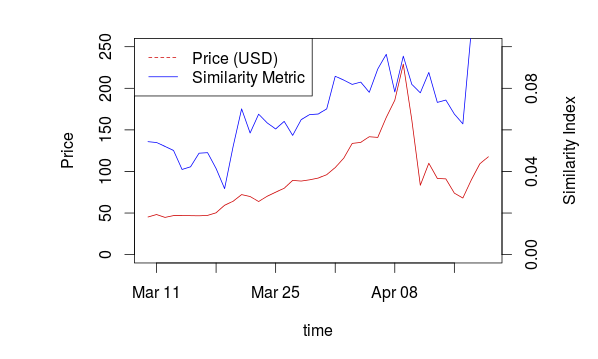
\includegraphics[width=\textwidth]{./Figures/pnc.png}
\caption{Daily transactions price correlation with network structure. The similarity index was calculated by RWGK }
\label{fig:RWGK}
\end{center}
\end{figure}

Although random walk kernels are still among the widely adopted graph kernels, one common disadvantage with them is that walks and paths do not capture information of the substructures present in the graph. The weak correlation as seen in the figure \ref{fig:RWGK} support our reasoning. Possibility of tottering \citep{Mahe2004} and halting \citep{Sugiyama2015} problem cannot be ruled out. This in turns focus our direction to use other graph kernels, free from above problem and can be scalable.

Next we use propagation kernels, whose design is motivated by the
iterative information propagation. They not only capture structural information, but can often adapt to the aforementioned issues of real world data. Adding to the same, they didn’t  suffer from the problem of halting and tottering \citep{Neumann2015}. Figure \ref{fig:PGK} plot the correlation between network structure and BTC/USD exchange price.

\begin{figure}[ht]
\begin{center}
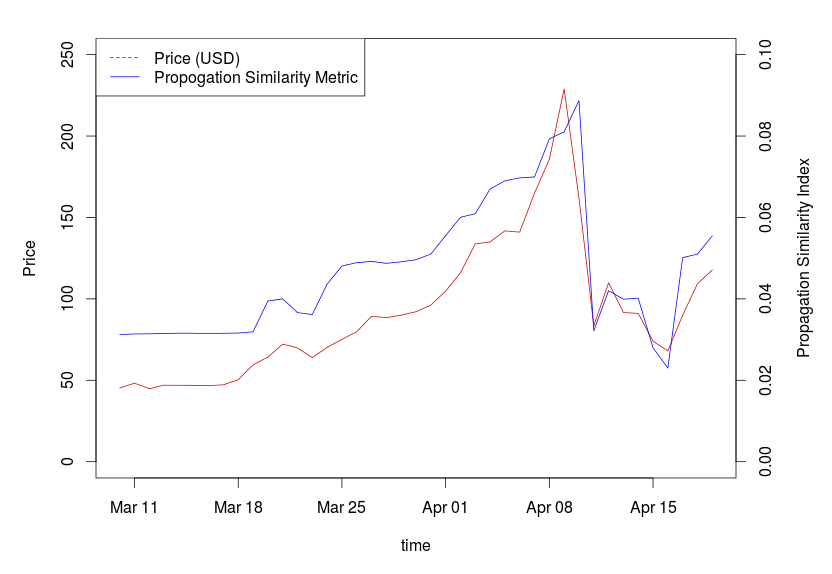
\includegraphics[width=\textwidth]{./Figures/PGK.png}
\caption{Daily transactions price correlation with network structure. The similarity index was calculated by PGK }
\label{fig:PGK}
\end{center}
\end{figure}

As expected figure \ref{fig:PGK} infer that the time-varying contribution of large scale transaction network correspondence with the market price of bitcoins, but there is still hope for the improvement, as graph is not smooth.
 

\section{Conclusions}

The purpose of this thesis is to offer an accurate and efficient similarity measure for dynamically changing large-scale graphs and structurally comparable graphs. By defining quantitative measure of transformation over time, in terms of similarity index using differnt kernels, we infer that there is correspondence between network structure and exchange price in bitcoin. The not so smooth graph direct our research to use other graph kernels. Our analysis of real-world transaction data from bitcoin  showcases a successful application of the method, which can further be employed in analyzing data from various fields.

\section{Summary}
This chapter review of representative graph kernels in the literature. By taking conventional and sophisticated graph kernels, this chapter defines   quantitative measure of transformation over time. The chapter concludes with not so smooth correspondence between network structure and exchange price in bitcoin, thus paving way for further investigation to other graph kernels.
%----------------------------------------------------------------------------------------

%% Chapter 4
\chapter{Graph Kernels} % Main chapter title

\label{Chapter4} % For referencing the chapter elsewhere, use \ref{Chapter1} 

\lhead{Chapter4. \emph{Graph Kernels}} % This is for the header on each page - perhaps a shortened title

%----------------------------------------------------------------------------------------
Kernels methods offer natural framework to study machine learning questions in different field, where graphs are used to model relationships between structure, with nodes representing objects and edges the relations between them. In this scenario, researcher direction leads to one important questions: “How similar are two graphs to each other?". To answer the above question, the kernels between graph was first proposed by G{\"a}rtner et al. \citep{Gartner2003} and later extended by Borgwardt et al.\citep{Borgwardt2005}. The graph kernels replace the explicit projection in feature space with the evaluation of a symmetric semi-definite positive similarity function. It can utilize infinite possible feature spaces by the learning algorithm with complexity of the kernel function, rather on the size of the feature space. Most kernel functions for graphs associate specific types of substructures to features, so the evaluation is then related to the number of common substructures between two graphs. The most common substructures widely used in the literature includes include random walks, paths, tree structures and rational kernels \citep{Vishwanathan2010}. Now, we review some of the representative graph kernels. 

\section{Random Walk Graph Kernels}
\label{sec:RWGK}

One of the popular graph kernel, random walk graph kernel \citep{Gartner2003, Kashima2003} counts matching walks in two input graphs. The basic idea behind this kernel to perform simultaneous random
walks between the vertexes of the graphs,  given a pair of graphs and count the number of matching paths.

\subsection{Computation}

Taking two graph $G_{1}, G_{2}$, let $E_{\times}$ denote the adjacency matrix
of their direct product $E_{\times} = E (G1 \times G2) $, and $V_{\times}$ denote the vertex set of the direct product  $V_{\times} = V (G1 \times G2) $. With a sequence of weights $\lambda = \lambda_{0}, \lambda_{1},...$
($\lambda_{i} \in R$; $\lambda_{i} \geq 0$ for all $i \geq N$) the direct product kernel is defined as:

%
\begin{equation}
K_{\times} (G_{1}, G_{2}) = \displaystyle\sum_{i,j=1}^{| V_{\times} |} \Bigg[ \displaystyle\sum_{k=0}^{\infty} \lambda_{k}E_{\times}^{k} \Bigg]_{ij}
\end{equation}
%

The graph kernel $K(G_{1}, G_{2})$ is computed efficiently computing matrix power series $\lim_{n \to \infty} \sum_{i=0}^{n} \lambda_{i}E^{i}$, which is explained in  Gartner et al. \citep{Gartner2003} by taking exponential and geometric series. The graph kernel is normalised to get similarity index in our case. In simple words, elegant computation involves, computing walk of length k by looking at the $k^{th}$ power of the adjacency matrix, then constructing direct product of the graph $G_{1}, G_{2}$ and counting walk on the product graph $K_{\times} (G_{1}, G_{2})$.  $E^{k} (i,j)$ = $c$ means that $c$ walks of length $k$ exist between vertex $i$ and vertex $j$. 

\subsection{Disadvantages}
Although random walk kernels and path based kernels
are still among the widely adopted graph kernels, It is prohibitively expensive, requiring $O(n_{6})$ runtime and suffers 
from the problem of tottering \citep{Mahe2004} and halting \citep{Sugiyama2015}. Other common disadvantage with them is that walks and paths do not capture information of the substructures present in the graph.

\subsection{Potential solutions}

The computation of the above was greatly improved by Vishwanathan et al. \citep{Vishwanathan2010} using iterative methods, including those based on Sylvester equations, conjugate gradients, and fixed-point iterations. Other improvements by Kang et al. \citep{Kang2012} takes account for just unlabeled graphs with the normalized weight matrix. Tottering problem was solved by  Mahe et al.\citep{Mahe2004} by doing special transformation on the input graphs, but it suffer from adverse computation time ($O(n)$ to $O(n_{2}$) and does not show a uniform improvement of classification accuracy. Replacing walk by path  Borgwardt et al.\citep{Borgwardt2005}, solved the tottering and  halting problem, but dense matrix representation for connected graphs, may lead to memory problems on large graphs. 

But the recent paper by  Sugiyama and Borgwart \citep{Sugiyama2015} claimed geometric random walk kernels suffers from the problem  referred to as halting: Longer walks are downweighted so much that the similarity score is completely dominated by the comparison of walks of length 1. This means that defining kernels for the graph is ongoing process, which keeps the improvements cycles on.

\section{Shortest Path Kernel on Graphs}

The foundation of shortest path graph kernels emerged because, paths do not suffer from tottering, as the number of self-loop-avoiding paths between all pairs of nodes of a given graph is useful for understanding the structure of the graph. But computing the number of such paths between all nodes is however a computationally hard task. Instead, only the number of shortest paths is counted  between node pairs in polynomial time avoiding cycles, thus is used as best structural measure in graph kernels \citep{Kriegel2005}.

\subsection{Methodology}
The first steps involves computing all-pairs-shortest-paths for $G_{1}$ and $G_{2}$ via Floyd-Warshall or Dijkstra’s algorithm. We then define graph kernel as a function $k(G_1,G_2)$ on pairs of graphs, which can be represented as an inner product $k(G_1,G_2) = \langle \phi(G_1), \phi(G_2) \rangle_{\mathcal{H}}$ for some mapping $\phi(G)$ to a Hilbert space $\mathcal{H}$, of possibly infinite dimension. Denoting $D(G)$ as the multi set of shortest distances between all node pairs in the graph $G$, we define  shortest path kernels two given graphs $G_1$ and $G_2$ as:

%
\begin{align}
K_{\rm SP}(G_{1}, G_{2})
=\sum_{d_1\in D(G_{1})}\;\sum_{d_2\in D(G_{2})}k(d_1,d_2),
\label{eq:SPKernel}
\end{align}
%
where $k$ is a positive definite kernel \citep{Borgwardt2005, Kriegel2005}.

\subsection{Advantages}
The shortest path graph kernels doesn't suffer  from tottering, and has  better accuracy on classification benchmarks. Runtime is in $O(n_{4})$, which includes computing all-pairs-shortest-paths for $G_{1}$ and  for $G_{2} \colon O(n_{3})$. Also, comparing all pairs of shortest paths from $G_{1}$ and  $G_{2} \colon O(n_{4})$. It is empirically faster than (fast) random walk kernels (probably due to graph size) \citep{Kriegel2005}.

\subsection{Disadvantages}

The complexity of order $O(n_{4})$  is too slow for large graphs. The essential step, dense matrix representation for connected graphs, may lead to memory problems on large graphs.

\subsection{Potential Solution}

The above problem of dense matrix representation was solved by new tree-based kernel for graphs \citep{Martino2012}. Graphs are decomposed into multisets of ordered Directed Acyclic Graphs (DAGs) and a family of kernels computed by application of tree kernels extended to the DAG domain. They provide richer representation of graph structure than walk-based approach, but their runtime grows exponentially with the recursion depth of the tree.

\section{Graphlet Kernels}
While using graph kernels, a practitioner is faced with some important dilemmas: Which graph kernels to be chosen for particular application?
If chosen, how good it capture graph similarity by being better
than others?  Is it cheap to compute? Unfortunately, all the above questions are too difficult to be answered, and no theoretical justification supports the selection of particular graph kernels.\citep{Yanardag2015B}.

The one way to look into the solutions of the above problem is efficiently computable representation that adequately captures the topology of the input graphs. Graph kernels do it by counting on the distribution of subgraphs of size $k$, refereed to as "graphlets".

\subsection{Description}

Using the notation from Yanardag and Vishwanathan paper \citep{Yanardag2015B}, we define graph as pair $G=(V,E)$ where $V = \left \{ v_1, v_2, \ldots,
  v_{|V|} \right \}$ is an ordered set of \emph{vertices} or
\emph{nodes} and $E \subseteq V \times V$ is a set of \emph{edges}.
Given $G = (V, E)$ and $H = (V_H , E_H )$, $H$ is a {\em sub-graph} of
$G$ iff there is an injective mapping $\alpha : V_H \rightarrow V$ such
that $(v, w) \in E_H$ iff $(\alpha(v), \alpha(w)) \in E$.  Two graphs $G
= (V, E)$ and $G' = (V', E')$ are {\em isomorphic} if there exists a
bijective mapping $g: V \rightarrow V'$ such that $(v_i, v_j) \in E$ iff
$(g(v_i), g(v_j)) \in E'$. {\em Graphlets} are small, connected,
non-isomorphic sub-graphs of a large network.

With clear notation, we now define graphlet kernels. Let $\mathcal{G}_{k} = \{ g_{1}, g_2, \ldots, g_{n_k} \}$ be the set of
size-$k$ graphlets where $n_k$ denotes the number of unique graphlets of
size $k$.  Given a graph $G$, we define $f_{G}$ as a normalized vector
of length $n_k$ whose $i$-th component corresponds to the frequency of
occurrence of $g_{i}$ in $G$:
%
\begin{align}
  \label{eq:gk}
  f_G = (\frac{c_1}{\sum_{j}^{n_k} c_j}, \cdots, \frac{c_{n_k}}{\sum_{j}^{n_k} c_j})^T.
\end{align}
%
Here $c_i$ denotes number of times $g_i$ occurs as a sub-graph of
$G$. Given two graphs $G$ and $G'$, the graphlet kernel $k_{g}$ is
defined as:
\begin{align}
  \label{eq:graphlet-kernel}
  k_{g}(G, G'):= f_{G}^{\top} f_{G'},
\end{align} 
which is simply the dot product between the normalized
graphlet-frequency vectors \citep{Yanardag2015B}.

\subsection{Problem}

The graphlet kernel described above uses induced sub-graphs of $k$ nodes as motifs in the vector representation, and computes the kernel via a dot product between these vectors.  As  the size of $k$ increases, the sparsity problem pitch in and most higher order graphlets will not occur in a given graph. This affect is diagonal dominance, where a given graph is similar to itself but not to any other graph in the dataset \citep{Yanardag2015B}. Also, more numerous lower order graphlets withlower values of k does not provide enough discrimination ability.

\subsection{Improvement}

To tackle the above problems, Yanardag and Vishwanathan \citep{Yanardag2015B} proposed  smoothing technique based on a novel extension of Kneser-Ney and Pitman-Yor smoothing techniques from
natural language processing to graphs. The smoothing algorithm  tackles the diagonal dominance problem by distributing the probability mass
across graphlets and preserve the dependency.
 


\section{Graphs Kernels with Continuous Attributes}
A plethora literature on graph kernels (including above) is devoted to discrete attributes graph structures. Out of them, most are not suited for non-discrete node labels since their computational efficiency
hinges on avoiding to consider matches between distinct
discrete labels. An alternative extend the definition of traditional graph kernels, and consequently derive a graph kernel, which is able to deal with complex and continuous node labels. The same was done by Martino et al. \citep{Martino2012} by extended tree kernels to continous attributes. An open challenge to develop a scalable kernel on graphs with continuous-valued node attributes was taken by Feragen et al. \citep{Feragen2013}. By taking convolution kernel counting sub-path similarities, they presented  GraphHopper kernel between graphs with real-valued edge lengths and any type of node attribute, including vectors. The detail description of graph kernels with contionus contributes is discussed in the next section.

\section{Propagation Kernels}
\label{sec:PGK}

Recent work on graph kernels tries to capture structural information encoded in node labels, attributes, and edge information to come up "propagation kernels", which can be used to construct kernels for many graph types, including labeled, partially labeled, unlabeled, directed, and attributed graphs \citep{Neumann2015}. Propagation kernels leverage the power of continuous node label distributions as graph features
and hence, enhance traditional graph kernels to efficiently handle partially labeled graph in a principled manner.

\subsection{Method}

Taking the help of propagation kernels \citep{Neumann2015}, We define a kernel $K\colon \cm{X} \times \cm{X} \to \mathbb{R}$ 
among graph instances $G^{(i)} \in \cm{X} $. The input space $\cm{X}$ comprises graphs $G^{(i)} = (V^{(i)},E^{(i)},\ell)$, where $V^{(i)}$ is the set of nodes and $E^{(i)}$ is the set of edges in graph $G^{(i)}$. Weighted adjacency matrices $A^{(i)} \in \mathbb{R}^{n_i \times n_i}$ represents and the label function~$\ell$ endows nodes with label and attribute information.
The similarity between two graphs $G^{(i)}$ and $G^{(j)}$ is to computed by comparing all pairs of nodes in the above two:
\begin{align}
 K(G^{(i)}, G^{(j)}) =  \sum_{v \in G^{(i)}} \sum_{u \in G^{(j)}} k(u,v),  \notag
\end{align}
where $k(u,v)$ is an arbitrary node kernel determined by node labels
and, if present, node attributes. It is defined in terms of the nodes' corresponding probability distributions $p_{t,u}$ and $p_{t,v}$, which we update and maintain throughout the process of information propagation.

The kernel contribution of iteration $t$ is defined by
\begin{align}
 K(G^{(i)}_t, G^{(j)}_t) =  \sum_{v \in G^{(i)}_t} \sum_{u \in G^{(j)}_t} k(u,v).
 \label{equ:kernel_contib}
\end{align}
The propagation kernels between labeled and attributed graphs are defined as:

\begin{align}
 k(u,v) = k_l(u,v) \cdot k_a(u,v),
 \label{equ:node_kernel}
\end{align}

where $k_l(u,v)$ is a kernel corresponding to label information and
$k_a(u,v)$ is a kernel corresponding to attribute information.  If no
attributes are present, then $k(u,v) = k_l(u,v)$.  The
$t_{\textsc{max}}$-iteration propagation kernel is now given by

\begin{align}
 K_{t_{\textsc{max}}}(G^{(i)}, G^{(j)}) = \sum_{t = 1}^{t_{\textsc{max}}} K(G^{(i)}_t, G^{(j)}_t).
 \label{equ:pk_kernel}
\end{align}


If node kernel is defined in the form 

\begin{align}
  k(u,v) = \left\{
  \begin{array}{l l}
    1\;\; &  \text{if } condition\\
    0\;\; &  \text{otherwise},
  \end{array} \right.
  \label{equ:dirac_kernel}
\end{align}

where $condition$ is an equality condition on the information of nodes
$u$ and $v$, we can compute $K$ efficiently by \emph{binning} the node
information, \emph{counting} the respective bin strengths for all
graphs, and \emph{computing a base kernel} among these counts.  That
is, we compute count features $\phi(G^{(i)}_t)$ for each graph and
plug them into a base kernel: $\langle \cdot,\cdot \rangle$

\begin{align}
 K(G^{(i)}_t, G^{(j)}_t) = \langle\phi(G^{(i)}_t),\phi(G^{(j)}_t)\rangle.
 \label{equ:feature_kernel}
\end{align}
 
 The above mathematical equations can be put in the form of algorithms \ref{algo:propKernel}.
 
 \begin{algorithm}[t]
  \caption{The general propagation kernel computation \citep{Neumann2015}.}
  \begin{algorithmic}
    \State \textbf{given:} graph database $\{G^{(i)}\}_i$, $\#$ iterations $t_{\textsc{max}}$, propagation scheme(s), base kernel $\langle \cdot, \cdot \rangle$
    \State $K \gets 0$, $initialize\;\, distributions\;\, P_0^{(i)}$
    \For{$t \gets 0\dotsc t_{\textsc{max}}$}
    \ForAll{graphs $G^{(i)}$}
    \ForAll{nodes $u \in G^{(i)}$}
    \State $quantize\;\;p_{t,u}$, where $p_{t,u} \text{ is } u\text{-th row in }P^{(i)}_t$ 			\Comment{bin node information}
    \EndFor
    \State $compute\;\;  \Phi_{i \cdot} = \phi(G^{(i)}_t)$  \Comment{count bin strengths}
    \EndFor
    \State $K \gets K + \langle \Phi, \Phi\rangle $ 	\Comment{compute and add kernel contribution}
    \ForAll{graphs $G^{(i)}$}
    \State $P^{(i)}_{t+1} \gets P^{(i)}_{t}$ 				\Comment{propagate node information}
    \EndFor
    \EndFor
  \end{algorithmic}
  \label{algo:propKernel}
\end{algorithm}

\subsection{Advantages}
There are two major benefit of using propagation kernels: The shelf propagation schemes as discussed above can be used to naturally construct kernels for labeled, partially labeled, unlabeled, directed, and attributed graphs. Also, by leveraging existing efficient and informative propagation schemes, propagationkernels can be considerably faster than state of the art approaches \citep{Neumann2015}.

\section{Recent Graph Kernels}

Other graphs kernels includes,  Optimal Assignment Kernels and Edit-Distance Kernel, which  are not positive definite in general; Subtree Kernel runtime grows exponentially with the recursion depth of the subtree like patterns; Cyclic Pattern Kernel restrict their attention to scenarios where the number of simple cycles in a graph dataset is bounded by a constant and Graphlet Kernel's common solutions not feasible on labeled graphs \citep{Vishwanathan2010}.  

Bai et al.\citep{Bai2015} developed a novel graph kernel by aligning the Jensen-Shannon (JS) representations of vertices, which addresses the drawback of neglecting the relative locations between substructures that arises in the R-convolution kernels. 

To solve the problem of graph structure at multiple different scales, Kondor and Pan \citep{Kondor2016} introduces, Multiscale Laplacian Graph kernels (MLG kernels), which has the Feature Space Laplacian Graph kernel (FLG kernel) with the  property that it can lift a base kernel
defined on the vertices of two graphs to a kernel between the graphs. 

In the recent KDD 2015 paper by Yanardag and Vishwanathan \citep{Yanardag2015} used language modeling and deep learning to learn latent representations of sub-structures for graphs. Their framework leverages the dependency information between sub-structures by learning their latent representations. Using three popular graph kernels, namely Graphlet kernels, Weisfeiler-Lehman subtree kernels, and Shortest-Path graph kernels, their models proves to be improves the classification accuracy, robust to random noise and computationally efficient. We discuss deep graph kernels in the next chapter with scholastic detail.

\section{Methodology}

Here, we present a method to efficiently measure the change
of a dynamic graph (bitcoin transaction graph) whose connectivity structure evolves over time with respect to changes in the exchange price of bitcoins. and quantative measure of the similarity of large-scale graph datasets along with justification for our method.

In simple word, given two graph $G_{1}, G_{2}$, we need to find similarity index $SI(G_{1}, G_{2})$, that lies between 0 and 1.

\subsection{Graph Dataset}

We parsed the transaction data from blockchain in the form \ref{table:TD}, which is automatically downloaded at the local machine, once Bitcoin Core is set-up. Once the data is loaded at SQL database, we extract the daily transaction for the month of March, 2003 to May, 2003 to capture maximum variation, as this period have two major bubbles. The resulting transaction network for the April, 2013 consists of 64,782 addresses with 100,952 edges.

\begin{center}
\begin{table}[ht]
\caption{Transaction Data Format} % title of Table
\centering % used for centering table
\begin{tabular}{c c c c c} % centered columns (4 columns)
\hline\hline %inserts double horizontal lines
$Transaction_{From}$ & $Transaction_{To}$ & $Value$ & $Timestamp$\\ [0.5ex] % inserts table
%heading
\hline % inserts single horizontal line
 &  &  & \\ % inserting body of the table
 &  &  &  \\ [1ex] % [1ex] adds vertical space
\hline %inserts single line
\end{tabular}
\label{table:TD} % is used to refer this table in the text
\end{table}
\end{center}

\subsection{Graph Kernel Calculation}

We use widely used random walk graph kernels (RWGK) to calculate similarity index. As RWGK suffers from various problem, which is then corrected by propagation graph kernels (PGK), we intend to use it too, so that fair comparison can be done. 

\subsubsection{Similarity Index: RWGK}

We take simple case of random walk graph kernels as defined in section \ref{sec:RWGK}. Taking two graph $G_{1}, G_{2}$, let $E_{\times}$ denote the adjacency matrix of their direct product $E_{\times} = E (G1 \times G2) $, and $V_{\times}$ denote the vertex set of the direct product  $V_{\times} = V (G1 \times G2) $. With a sequence of weights $\lambda = \lambda_{0}, \lambda_{1},...$
($\lambda_{i} \in R$; $\lambda_{i} \geq 0$ for all $i \geq N$) the direct product kernel is defined as:

%
\begin{equation}
K_{\times} (G_{1}, G_{2}) = \displaystyle\sum_{i,j=1}^{| V_{\times} |} \Bigg[ \displaystyle\sum_{k=0}^{\infty} \lambda_{k}E_{\times}^{k} \Bigg]_{ij}
\label{eq:1}
\end{equation}
%
The graph kernel $K(G_{1}, G_{2})$ is computed efficiently computing matrix power series $\lim_{n \to \infty} \sum_{i=0}^{n} \lambda_{i}E^{i}$, which is explained in  G{\"a}rtner et al.\citep{Gartner2003}.

The similarity index $SI_{RWGK}(G_{1}, G_{2})$ is calculated by normalising graph kernels. The method is implemented in Python by converting readly available Matlab code \citep{Kashima2003}.

\subsection{Similarity Index: PGK }

Propagation graph kernel is calculated by method as discussed in section \ref{sec:PGK}.

\begin{align}
 K(G^{(i)}_t, G^{(j)}_t) = \langle\phi(G^{(i)}_t),\phi(G^{(j)}_t)\rangle.
\label{eq:2}
\end{align}

The similarity index $SI_{PGK}(G^{(i)}_t, G^{(j)}_t)$ is calculated by normalising graph kernels. The method is implemented in Python by converting readly available Matlab code \citep{Neumann2015}.

Note that graph similarity reflecting overall graph structure
ends up lying in between 0 and 1, as governed by normalised version of Eq. \ref{eq:1} and \ref{eq:2}.

\section{Results and Discussion}

To investigate the connection between the network structure and
macroscopic properties (i.e. the exchange price) in the Bitcoin network, we plot similarity index and BTC/USD exchange price. This in turn, offer an accurate and efficient similarity measure for dynamically changing large scale graphs and structurally comparable graphs. 

We first plot the similarity index calculated by popular RWGK and BTC/USD exchange price.

\begin{figure}[ht]
\begin{center}
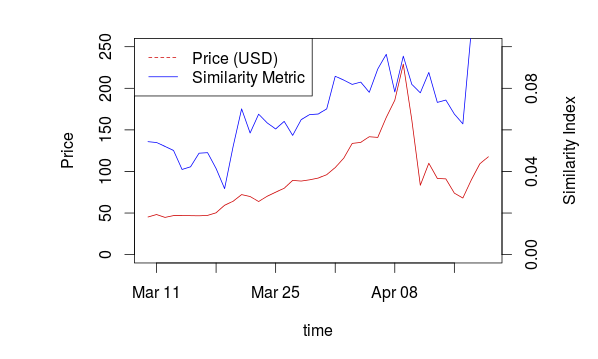
\includegraphics[width=\textwidth]{./Figures/pnc.png}
\caption{Daily transactions price correlation with network structure. The similarity index was calculated by RWGK }
\label{fig:RWGK}
\end{center}
\end{figure}

Although random walk kernels are still among the widely adopted graph kernels, one common disadvantage with them is that walks and paths do not capture information of the substructures present in the graph. The weak correlation as seen in the figure \ref{fig:RWGK} support our reasoning. Possibility of tottering \citep{Mahe2004} and halting \citep{Sugiyama2015} problem cannot be ruled out. This in turns focus our direction to use other graph kernels, free from above problem and can be scalable.

Next we use propagation kernels, whose design is motivated by the
iterative information propagation. They not only capture structural information, but can often adapt to the aforementioned issues of real world data. Adding to the same, they didn’t  suffer from the problem of halting and tottering \citep{Neumann2015}. Figure \ref{fig:PGK} plot the correlation between network structure and BTC/USD exchange price.

\begin{figure}[ht]
\begin{center}
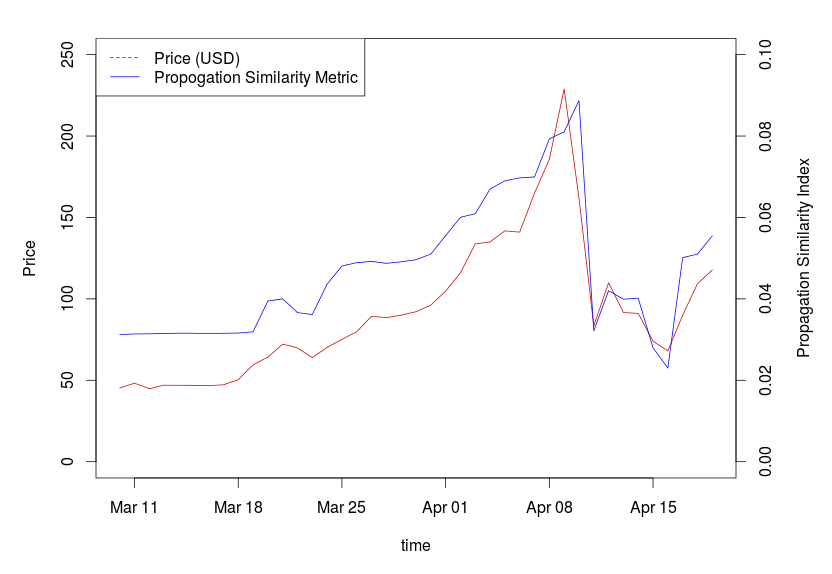
\includegraphics[width=\textwidth]{./Figures/PGK.png}
\caption{Daily transactions price correlation with network structure. The similarity index was calculated by PGK }
\label{fig:PGK}
\end{center}
\end{figure}

As expected figure \ref{fig:PGK} infer that the time-varying contribution of large scale transaction network correspondence with the market price of bitcoins, but there is still hope for the improvement, as graph is not smooth.
 

\section{Conclusions}

The purpose of this thesis is to offer an accurate and efficient similarity measure for dynamically changing large-scale graphs and structurally comparable graphs. By defining quantitative measure of transformation over time, in terms of similarity index using differnt kernels, we infer that there is correspondence between network structure and exchange price in bitcoin. The not so smooth graph direct our research to use other graph kernels. Our analysis of real-world transaction data from bitcoin  showcases a successful application of the method, which can further be employed in analyzing data from various fields.

\section{Summary}
This chapter review of representative graph kernels in the literature. By taking conventional and sophisticated graph kernels, this chapter defines   quantitative measure of transformation over time. The chapter concludes with not so smooth correspondence between network structure and exchange price in bitcoin, thus paving way for further investigation to other graph kernels.
%----------------------------------------------------------------------------------------
 

%----------------------------------------------------------------------------------------
%	THESIS CONTENT - CHAPTER5
%----------------------------------------------------------------------------------------

%\mainmatter % Begin numeric (1,2,3...) page numbering

\pagestyle{fancy} % Return the page headers back to the "fancy" style

% Include the chapters of the thesis as separate files from the Chapters folder
% Uncomment the lines as you write the chapters

% Chapter 5
\chapter{Deep Graph Kernels} % Main chapter title

\label{Chapter5} % For referencing the chapter elsewhere, use \ref{Chapter1} 

\lhead{Chapter5. \emph{Deep Graph Kernels}} % This is for the header on each page - perhaps a shortened title

%----------------------------------------------------------------------------------------
Over recent years, graph kernels are one the promising candidate for problem related to graph isomorphism. Graph Kernels are based on the comparison of graph-substructures via kernels. The graph-substructure including walks, path, subtrees, graphlets and cyclic patterns have been widely used to construct kernels. However, kernels on these substructures are either computationally expensive, NP-hard to determine, limited in their expressiveness or applicable to  just a small
subset of graphs rather all graphs. Existing graph kernels have difficulties with reaching at least one of these goals.

An emerging line of research, consisting in designing meaningful kernels on structured data, produced promising results in cheminformatics, bioinformatics, computer vision and natural language processing. The graph kernels together with techniques from natural language processing and computer vision  have recently received an increased attention, and showed good performances for classification of small molecules \citep{Mahe2004}. In very recent years, lots of research has been developed around deep learning architectures that allow for higher level abstractions for representing and understanding graph data \citep{Perozzi2014}.

Deep learning is method based on learning representations of data, which attempt to model high-level abstractions in data by using multiple processing layers, with complex structures or otherwise, composed of multiple non-linear transformations. By using deep learning, Perozzi et al.\citep{Perozzi2014} proposed DeepWalk, which uses local information obtained from truncated random walks to learn social representations of vertices of graphs. Motivating from DeepWalk, Yanardag and Vishwanathan \citep{Yanardag2015} work focuses on learning similarities
between structured objects, such as graphs and strings, instead of nodes of the single graph. However, the adoption of deep learning in graphs isomorphisms has not been adequately investigated yet. 

\section{Background}

Deep Graph Kernels \citep{Yanardag2015} is not so deep learning frame work to learn latent representations of sub-structures for graphs, which are not independent. The framework leverage on the dependency information between sub-structures by learning their latent representations. To motivate our discussion of using deep graph kernels, we first try to explain the problem associated with general graph kernels representation.

\section{Representation Problem}

Graph Kernels are produced using R-convolution, where a graph is to recursively decomposed into into “atomic” sub-structures to define a kernels between them.  Mathematically, It can be expressed as:

%
\begin{equation}
K(G_{1}, G_{2}) = {\Bigg \langle \Phi(G_{1}), \Phi(G_{1}) \Bigg \rangle}_{\mathcal{H}}
\label{eq:dgk}
\end{equation}
%

Where, $\Phi(G)$ is denote a vector which contains counts of atomic sub-structures. 

The representation in the equation \ref{eq:dgk} suffers from two basic problems. First, the sub-structure are not independent. Second, the dimension of the feature space often grows exponentially, as substructure grows, which leads to "diagonal dominance" \citep{Kandola2003}, that is, a given graph is similar to itself but not to any other graph in the dataset. But, we need a kernel matrix where all entries belonging to a class are similar to each other, and dissimilar to everything else. 

\section{Deep Framework}

To alleviate the representation problem, we define alternative graph kernel as:

%
\begin{equation}\label{eq:pdgk}
K(G_{1}, G_{2}) = \Phi(G_{1})^{T} \mathcal{M} \Phi(G_{1})
\end{equation}
%
 
where $\mathcal{M}$ represents a $|\mathcal{N}|\times |\mathcal{N}|$ positive semi-definite matrix that encodes the relationship between sub-structures and $\mathcal{N}$ represents the vocabulary of sub-structures obtained from the training data. Now, the important task is design $\mathcal{M}$, which can be computed by learning latent representations of sub-structures or by edit-distance relationship between sub-structures.

\section{Methodology} 

The $\mathcal{M}$ is computed by learning  the latent representations of
sub-structures by techniques such as Neural language models,  Continuous bag-of-words (CBOW) and Skip-gram model (SG) \citep{Yanardag2015}.

\subsection{Skip-Gram}
First, we review the representative Skip-Gram \citep{Milkov2013} \footnote{The google tool, \textit{Word2Vec} provides a fast, multi-threaded implementation of both SG and CBOW:https://code.google.com/p/word2vec/}. architecture in language modelling before transforming the ideas to learn representations of sub-structures. 

The SG model maximizes co-occurrence probability among the words that appear within a given window.  More precisely, SG model tries to minimize the following objective function: 
%
\begin{equation}
\mathcal{L}_{SG} = \sum_{t=1}^{T} \log P(w_{t-c}, \cdots , w_{t+c}|w_{t})
\label{eq:SG}
\end{equation}
%
where, $P(w_{t-c}, \cdots , w_{t+c}|w_{t})$ is computed as $\prod_{-c\leq j\leq c, j \neq 0} P(w_{t+j}|w_{t})$. Furthermore, 

%
\begin{equation}
P(w_{t+j}|w_{t}) = \frac{\exp(v^{\intercal}_{{w}_{t}} v^{\prime}_{{w}_{t}})}{\sum_{w=1}^{\mathcal{V}}\exp (v^{\intercal}_{{w}_{t}} v^{\prime}_{{w}_{t}})}
\end{equation}
%

Hierarchical softmax or negative sampling are two efficient algorithms that are used in training SG and CBOW  \citep{Yanardag2015}.

\section{Deep Graph Kernels}

The language modeling and deep learning techniques was used to compute $\mathcal{M}$ with intuition that different sub-structures compose graphs in a similar way that different words form sentences when used together. The list of decomposed sub-structures for each graph is then treated as a sentence that is generated from a vocabulary $\mathcal{V}$  where vocabulary $\mathcal{V}$ simply corresponds to the unique set of observed sub-structures in the training data. 

The linear co-occurrence relationship of sub-structure is created using modified random sampling scheme, taking account of neighborhoods. That is, whenever we randomly sample a graphlet $G$, we also sample its immediate neighbors. Then is corpus is generated according to particular graph kernels, for example, for shortest graph kernels, whenever shortestpath sub-structure is generated, all possible shortest-path sub-structures are also collected that share the same source node, and treat them as co-occurred.

\subsection{Corpus Generation}

Most of the graph kernels \citep{Vishwanathan2010} are designed for unlabeled graphs or graphs with a complete set of discrete node labels
, but graphs with continuous node attributes is catching up fast \citep{Feragen2013}. But these graph kernels can only handle graphs with complete label or attribute information in a principled manner. These may be efficient, but for specific graph and if flexible, computation is memory and/or time consuming. The propagation kernels by  \citep{Neumann2015} overcomes all the above problems. We exploit the propagation kernels in the deep framework to have similarity index between two graph. The propagation kernels measure the similarity between two graphs by comparing node label or attribute distributions after each step of an appropriate random walk.

The corpus is generated for propagation kernels \citep{Neumann2015}, which is explained in section \ref{sec:PGK}. Since, the propagation kernels are based on monitoring how information spreads through a set of given graphs. We use early-stage distributions from propagation
schemes such as random walks to capture structural information encoded in node labels, attributes, and edge information. In simple words, propagation kernels intuitively count common sub-distributions induced
after each iteration of running inference in two graphs. We collect all possible sub-distributions that share the same source node, and treat them as co-occurred. Therefore, sub-distributions which have similar labels will acquire similar representations. We differ from earlier studies in using propagation kernels, which is efficient than random walk, shortest path, graphlet and Weisfeiler-Lehman subtree kernel.

\subsection{Model Building and Training}
\label{ssec:MBT}
Once corpus is generated, the model is build by using  Skip-gram algorithms and trained with negative sampling as explained in the base reference \citep{Yanardag2015}. 

If $s$ represent an arbitrary sub-structure from a vocabulary $\mathcal{V}$, and $\phi_{s}$ represent learned vector representation of $s$. Matrix $\mathcal{M}$ is calculated such that, each entry on the diagonal is $\mathcal{M}_{ii}$ computed as $\big \langle \phi_{i},\phi_{i} \big \rangle$ where $\phi_{i}$ corresponds
to learned d-dimensional hidden of sub-sequence $i$ and $\mathcal{M}_{ii}$
where $i = $j and $1 \leq i \leq |\mathcal{V}|$ (resp. $j$). After computing the $\mathcal{M}$ matrix, it is plugged in Equation \ref{eq:pdgk} to get deep graph kernels. The similarity index $SI_{DGP}(G_{1}, G_{2})$ is calculated by normalising the \ref{eq:pdgk}.


\subsection{Experiments}
We compare our framework with the representative instances of
major families of graph kernels as discussed in \citep{Yanardag2015}. The similarity index is calculated as discussed in section \ref{ssec:MBT}. The Matlab code of the propagation kernels was obtained from \citep{Neumann2015}, which was then coded in python. The correlation between transaction network structure and market price is depicted by figure \ref{fig:ds}. It shows better correlation with the network, as compared to similarity index calculated by other graph kernels without using deep framework. 

\begin{figure}[ht]
\begin{center}
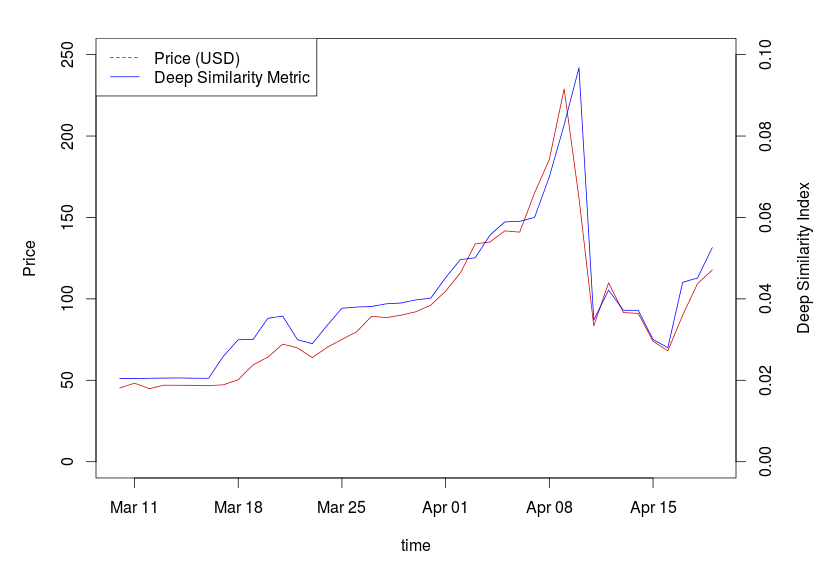
\includegraphics[width=0.8\textwidth]{./Figures/ds.png}
\caption{Deep Similarity}
\label{fig:ds}
\end{center}
\end{figure}

\section{Result and Discussions}
As per Bitcoin’s ”Metcalfe’s Law”, there is strong correlation between
market cap (transactions/day) and the square of the number of
transactions. As our graph is weighted network, where weight
represents the transactions between two agents, our results too
supports Metcalfe’s Law. We are able to show how structural changes in the network accompany significant changes (Quantitative Measure) in the
exchange price of bitcoins.

\section{Conclusions}
 In this study, we extend the quite novel framework for graph kernels inspired by latest advancements in natural language processing and deep learning. We extend the seminal work \citep{Yanardag2015} by introducing propagation kernels, which takes account of attributed graphs with continuous values. As expected, our deep graph kernels outperforms its best base variants in terms of capturing correlation between newtork structure and market price.
 
\section{Summary}
This chapter propose a general framework that learns hidden representations of sub-structures used in graph kernels, inspired
by deep graph kernels \citep{Yanardag2015}. Then, the framework  is demonstrated on propagation kernels, which performs better than normal kernels. The above framework is applied to derive deep variants of
string kernels. Then new graph kernel is used to calculate similarity index, which is plotted to find correlation between network structure and market price.

%----------------------------------------------------------------------------------------



%% Chapter 2
\chapter{Bitcoin Transaction Dynamics } % Main chapter title

\label{Chapter2} % For referencing the chapter elsewhere, use \ref{Chapter2} 

\lhead{Chapter 2. \emph{Bitcoin Transaction Dynamics}} % This is for the header on each page - perhaps a shortened title

%----------------------------------------------------------------------------------------
\section{Introduction}

Bitcoin is a decentralized peer to peer electronic payment system in which transactions are performed with no central authority or banks to authorize it. The Bitcoin transactions management and its issuance is carried out collectively by the network. The first Bitcoin specification and proof of concept was published by Satoshi Nakamoto \citep{Nakamoto2008} in 2009 cryptographic mailing list. Bitcoin can also be seen as the most prominent triple entry bookkeeping system in existence. Since then, the community has grown exponentially with many developers working on Bitcoin.


\section{Bitcoin}
\label{sec:bitcoin}
Bitcoin payments use public keys encryption, where, payers and payees are identified by hashed public keys of their Bitcoin wallets. The public keys are generated by ECDSA (Elliptic Curve Digital Signature Algorithm), based on calculations of elliptical curves over finite space. Suppose, Alice sends "$x$" coins to Bob, then an unencrypted transaction attaching Bob's public key is broadcast over the Bitcoin network using her private key. The signature on transaction verifies all users for its authenticity (current owner of coin) by looking at complete history of transactions, called {\it blockchain}. It is essential element in bitcoin architecture, which verifies the legitimacy of ability (sufficient bitcoins) of Alice paying Bob.

\subsection{Blockchain}


The complete record of transactions is in a coded form in a data structure called {\it blockchain}, which is a sequence of records called {\it blocks}. Each block contains a group of transactions that have been sent since the previous block, with integrity check all the way back to the first one, the genesis block.

Any users enter the Bitcoin system by trading non-digital currencies at Bitcoin market exchange, or by mining coins, which involves solving a cryptographically hard problem for which he/she is suitably rewarded a fixed number of Bitcoins  and transactions is validated on the network. The working of mining, core to {\it blockchain}, is mathematically explained better by Johannes et al. \cite{Johannes2015}. The network of peers, called miners, are the agents using computers, who actually add the blocks to the blockchain. Taking example of Alice sending "$x$" coins to Bob from section \ref{sec:bitcoin} by broadcasting over network. The miners receives copies of all transactions as they are generated, including Alice's copy. The blockchain is examined to investigate the history of the bitcoins involved in each transaction. If the proposed transaction from the Alice has sufficient bitcoin credit, then it is accepted for incorporation into the block that the miner is currently working on. 


Identifying each transaction with a double SHA-256 hash, the transactions is gathered together. Then by using miners hashes,together with the hash that is at the current head of the blockchain, as inputs to the cryptographic problem is solved by miners, with rewards of 25 bitcoins in 10 minutes \cite{Johannes2015}. At first, miner~$M$ computes a block hash~$h$ over a unique ordering of the hashes of all the transactions that it is intending to incorporate into its next block $B$.  Then, input of the block solution $s_{i-1}$ is taken at the head of its current version of the {\it blockchain}. If we concatenate the strings by the symbol $+$, the cryptographic problem that $M$ has to solve is: compute a SHA-256 hash
%
\begin{equation} \label{eq:2.1}
s_i = (n + h + s_{i-1}),
\end{equation}
%
such that $s_i$ has at least a specified number~$x$ of leading zeros where $x \sim 64$. 

Once mined, the new block is communicated by broadcasting newly-discovered
blocks via a peer-to-peer network to add the new block at blockchain at each peer using blockchain protocol rules. This makes blockchain as a public ledger, recording  every Bitcoin payment ever made. The simplified version of the whole process is represented in below illustration \ref{fig:blockchain}.

\begin{figure}[ht]
\begin{center}
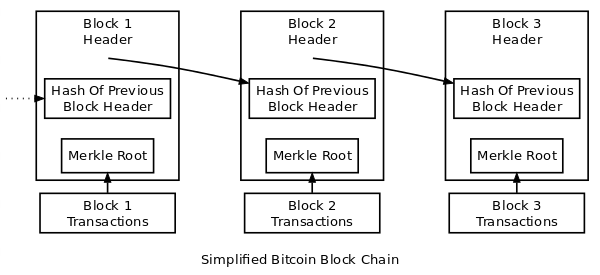
\includegraphics[width=0.8\textwidth]{./Figures/blockchain.png}
\caption{Simple Blockchain \citep{Blockchain2016}}
\label{fig:blockchain}
\end{center}
\end{figure}
The transaction data part of a block consists of one or more new transactions. While the merkel root of the merkle tree contains  hashed copies of each transaction, and the hashes are then paired, hashed, paired again, and hashed again until a single hash remains. The chaining of blocks together and storing the hash of the previous block’s header ensures a transaction cannot be modified without modifying the block that records it and all following blocks. The same goes with the transaction, which are also chained together. A single transaction can create multiple outputs, which  are tied to transaction identifiers (TXIDs), the hashes of signed transactions. Also, the outputs of all transactions included in the block chain can be categorized as either Unspent Transaction Outputs (UTXOs) or spent transaction outputs \ref{fig:block_t}. The first one of these transactions called a generation transaction, which should collect and spend the block reward (comprised of a block subsidy and any transaction fees paid by transactions included in this block). All these transactions are encoded into blocks in binary rawtransaction format, making it difficult for researchers to extract in simple relational database format, to get transaction graph.

\begin{figure}[ht]
\begin{center}
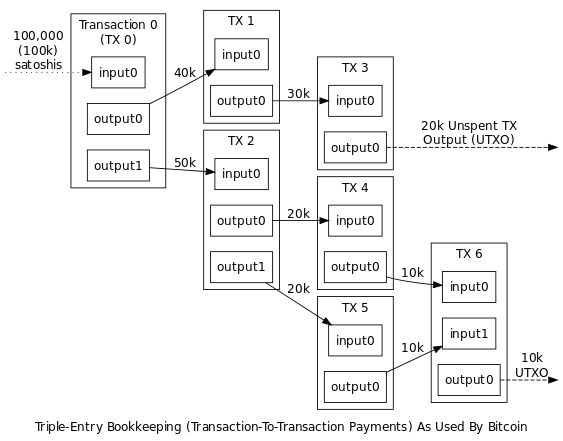
\includegraphics[width=0.8\textwidth]{./Figures/block_t.png}
\caption{Blockchain Transaction \citep{Blockchain2016}}
\label{fig:block_t}
\end{center}
\end{figure}

\section{Related Work}
The possibility to analyze agent resolved transactions in any market is limited by the scarcity of available data, as this kind of information is usually considered highly sensitive. But with the publicly available blockchain at every machine allows researchers to reconstruct the network of transactions and extract the time and amount of each payment. There are many research studies that concerns bitcoin transaction network using network analysis, machine learning and statistical physics techniques.

Parsing four (2009-2013) years data from bitcoin's  blockchain, Kondor et al. \citep{Csabai2014}  analyze the structure of the transaction network by measuring network characteristics over time, such as the degree distribution, degree correlations, clustering and money movement. Using the same data, they in their different paper \citep{Kondor2014} analyze changes in the structure of the subgraph induced by the most active users. They were  able to show find correlation between structural changes in the network and exchange price of bitcoins. But with exponential increase in the number of transaction over years, they method seems obsolete , as it is difficult to scale with their endorsed methods.

Reid and Harrigan \citep{Reid2013} linked addresses belonging to the same entity using external information. The using techniques such as context discovery and flow analysis, they investigate an alleged theft of Bitcoins. By running the Union-Find algorithm, Ron and Samir \citep{Ron2013}  associated the 3,120,948 addresses with 1,851,544 different entities to understand behaviour of users. Spagnuolo \citep{Spagnuolo2013} released open source project Bitiodine, which was able to cluster addresses and classify them using a dataset partially obtained in an automatic fashion, using scrapers for major web sources of bitcoin addresses. On the similar line, other paper \citep{Fleder2015} investigates bitcoin transaction-graph-annotation, which is capable of tracing and clustering user activity.

Most of the  previous research employed data collected from old Bitcoin- client Bitcoin 0.8 later, the newer bitcoin clients indexed the full blockchain using LevelDB instead making the publicly available bitcointools obsolete. Adding to the same, the nearing 300,000 transactions/day in 2015 gives really hard time to earlier algorithms to scale, thus motivating us to develop new techniques to parsing data from blockchain, reconstructing network and doing analysis.

\section{Data}
\label{data}
The blockchain is a transaction database of the Bitcoin.  Once Bitcoin core is setup at local machine, blockchain is automatically downloaded. Every full node participating in the Bitcoin network has the same copy. As of now there is more than 60 GB of Bitcoin blockchain dataset, which makes it difficult to parse the raw blockchain data. Most of the previous studies \citep{Ron2013} employed a forked version of bitcointools \footnote{\url{https://github.com/gavinandresen/bitcointools}}, but from the bitcoin clients 0.8 version, it indexed the full blockchain using LevelDB instead making the publicly available bitcointools obsolete. Other well know open source blockchain parser like blockparser \footnote{\url {https://github.com/znort987/blockparser}}, BitIodine \citep{Spagnuolo2013} etc are almost undocumented projects, where some appear to not even work. A paper \citep{Fleder2015} led me to BitcoinArmory project, which requires a dozen of manual interventions to get installed, but still doesn’t work.

We then started to look for ready-made SQL database, which pointed to BitcoinABe. This python based library reads the Bitcoin block file, transforms and loads the data into a SQL database \ref{fig:SQL}. But, Its takes more than two weeks to dump the data, which was not feasible option. We downloaded postgres database dumps of the bitcoin-ruby-blockchain database generated by webbtc \footnote{\url{http://dumps.webbtc.com/bitcoin/}}. Then, with slight modification to open repository BitIodine \citep{Spagnuolo2013} code, we parsed through the blockchain, and wrote wrapper classes that extracted the relevant information required to construct the transaction graph. The market price data was scarped from website \url {https://blockchain.info/} to plot graphs in R.

\section{Bitcoin Transaction Network}

Before getting the transaction network, we first define our graph, which acts as input to further mathematical application.

\begin{definition}
We consider weighted labelled graph. That is, a
graph $G=(V,E,\ell)$ is represented by a set of $|V|=n$ vertices, a
set of edges $E$ specified by a weighted adjacency matrix $A \in
\bb{R}^{n \times n}$, and a label function $\ell\colon V \rightarrow
\cm{L}$ with $\cm{L} = \left( [k], \R^D \right)$, where $k$ is the
number of available node labels and $D$ is the dimension of the
continuous attributes.  Given $V = \{v_1,v_2,...,v_n\}$, \emph{node
  labels} $\ell(v_i)$ are represented by nominal values and
\emph{attributes} $\mathbf{x}_i \in \bb R^D$ are represented by
continuous vectors. In a transaction graph, addresses are nodes, transactions are edges and weight is BTC.
\label{def:graph}
\end{definition}

With the overall transactions records parsed from the blockchain in human readable form, we construct a a weighted directed transaction graph that gives an intuition towards the flow of Bitcoins from one key to the other,the directed edge represents a particular transaction from a source address to a target address and weight represents the value of the transactions. For our experiments, we constructed graphs for more than two years (March, 2013 to December, 2015) to capture major bubble in Bitcoin history. Figure \ref{fig:dt} represent daily transaction graph for a typical day on April 8, 2013.

\begin{figure}[ht]
\begin{center}
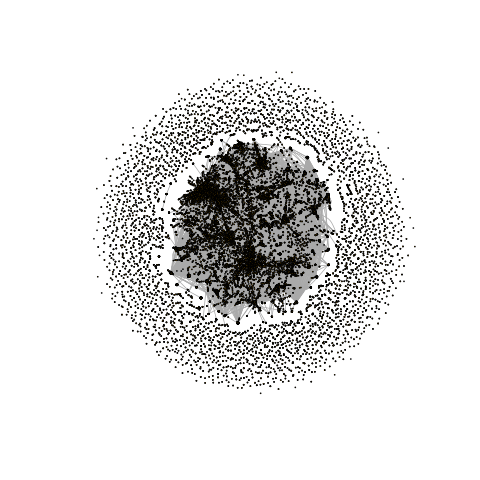
\includegraphics[width=\textwidth]{./Figures/dt.png}
\caption{ Daily transaction graph for a typical day (April 8, 2013)}
\label{fig:dt}
\end{center}
\end{figure}

\section{Transaction Dynamics}
The validation of the data parsed from our tool is then checked by
reproducing the ”Mathew Effect” phenomenon from the seminal work of Kondor et al. \citep{Csabai2014} paper’s using their original matlab code, but with our own data. The authors of the above papers are curator of whole blockchain up to 2014.10.19. (326,027 blocks), which is benchmark in quality. The similar figure confirms the high quality of our data.

To capture the transaction  dynamics in the bitcoin, we analyze the dynamics of money flow on the transaction network, as discussed in the paper \citep{Csabai2014}. We try to support popular hypothesis in economics having roots in preferential attachment, called Matthew effect or the "rich get richer phenomenon". It states that the growth of the wealth of each individual is proportional to the wealth of that individual \citep{Csabai2014}.

We assume that the number of bitcoins associated with node $n$ at time $t$ is given by $b_{n}(t)$. The difference between the balance of each
address at the end and at the start of each month is calculated. Then the difference in function of the starting balances is plotted in figure \ref{fig:dynamics}. The  positive correlation between balance and the average growth indicates the "rich get richer" phenomenon in bitcoin.

\begin{figure}[ht]
\begin{center}
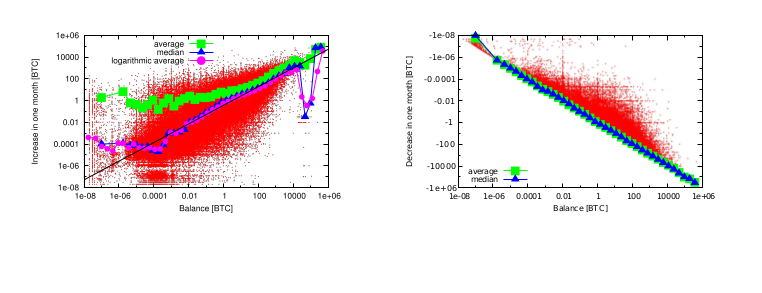
\includegraphics[width= \textwidth]{./Figures/dynamics.png}
\caption{ Matthew Effect}
\label{fig:dynamics}
\end{center}
\end{figure}

The figure \ref{fig:dynamics} is reproduced from Kondor's paper \citep{Csabai2014}, using our own data where Increase (left) and decrease (right) of node balances in one month windows as a function of their balance at the beginning of each month is represented. The representation in the picture follow the following colors: the raw data (red), the average (green), median (blue) and logarithmic average (magenta). The later three are calculated for logarithmically sized bins. The power-law fit for the double logarithmic data is represented by black line.

\subsection{Silk Road Arrest}

The Silk Road, under the alias of “Dread Pirate Roberts” (DPR) was known as an anonymous marketplace, a Black Market operated as a hidden service only accessible through Tor, where people who use bitcoins were able to buy and sell drugs, art, weapons etc. anonymously, without the risk of being tracked. It was founded by Ross William Ulbricht in February in 2011, but in October 2013 FBI closed the Silk Road and arrested Ulbricht. The FBI  seized approximately 173,600 BTC in two phase. At the first go 29,600 BTC held in a so called hot wallet were seized and an additional 144,000 BTC were seized using two addresses \footnote{1F1tAaz5x1HUXrCNLbtMDqcw6o5GNn4xqX, 1FfmbHfnpaZjKFvyi1okTjJJusN455paPH} controlled by the FBI. 

We illustrates the event using transaction network \ref{fig:silk} realised in gephi. Each vertex represents a user, where address is mapped to the user. Each directed edge between a source and a target represents a flow of Bitcoins from a public-key belonging to the user corresponding to the source to a public-key belonging to the user corresponding to the target. 

\begin{figure}[ht]
\begin{center}
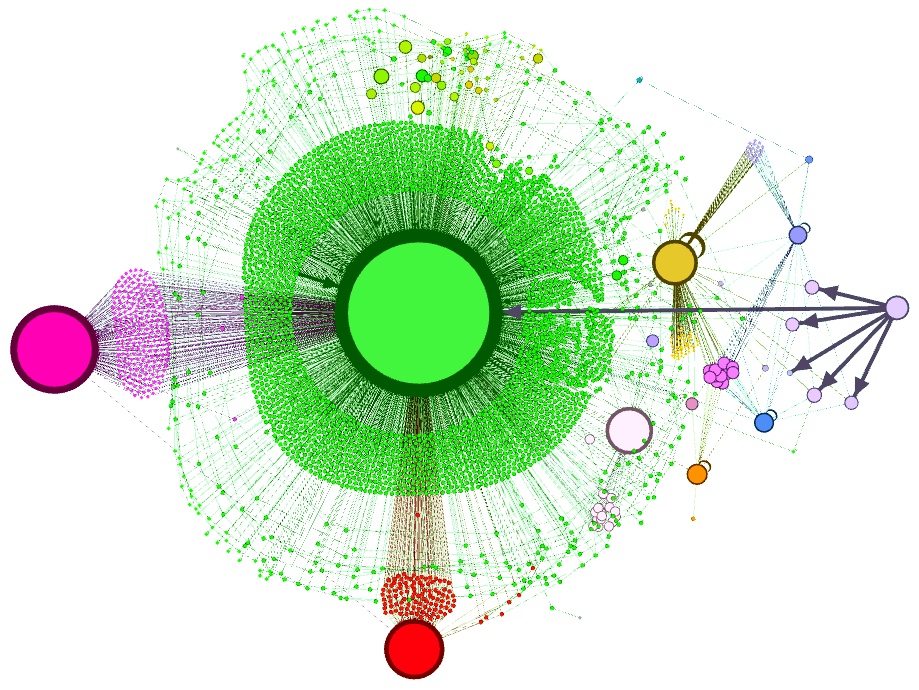
\includegraphics[width=0.7\textwidth]{./Figures/silk.png}
\caption{ Silk Road Arrest}
\label{fig:silk}
\end{center}
\end{figure}

Although in this scenario involves manual investigation by web scraping , it would have been difficult to find significant links manually, given the millions of nodes involved.

\section{Summary}
This chapter introduces Bitcoin, its working detail by explaining the protocol of blockchain, which contains all the history of transactions in the bitcoin. With enough knowledge about working of bitcoin, the related work in bitcoin transaction network is the discussed with the pros and cons. The data preparation staged is discussed to get the transaction network, an input to our mathematical model in coming chapters. The case study of silk road arrest is illustrated with the transaction graph. Transaction dynamics is reproduced from know studies to validate the parsed data, concludes the chapter. 
%----------------------------------------------------------------------------------------
%	THESIS CONTENT - CHAPTER6
%----------------------------------------------------------------------------------------

%\mainmatter % Begin numeric (1,2,3...) page numbering

\pagestyle{fancy} % Return the page headers back to the "fancy" style

% Include the chapters of the thesis as separate files from the Chapters folder
% Uncomment the lines as you write the chapters

% Chapter 6
\chapter{Conclusion and Future Scope} % Main chapter title

\label{Chapter6} % For referencing the chapter elsewhere, use \ref{Chapter1} 

\lhead{Chapter6. \emph{Conclusion and Future Scope}} % This is for the header on each page - perhaps a shortened title

%----------------------------------------------------------------------------------------

\section{Conclusions}
\begin{enumerate}

\item The enormous blockchain (60 GB as of now) and the newer bitcoin clients indexing the full blockchain using LevelDB had made earlier public available software obsolete. The thesis develops an open source blockchain parsing tools to extract agent resolved data, which can be used to extend the stucked research in bitcoin transaction dynamics.

\item The validation of the data parsed from our tool is then checked by
reproducing the ”Mathew Effect” phenomenon from prominent paper using their original matlab code, but with our own data. The transaction dynamics in the bitcoin as money flow on the transaction network, support popular hypothesis in economics having roots in preferential attachment, called Matthew effect or the "rich get richer phenomenon".

\item By using the agent resolved data, the case study of silk road arrest is illustrated with the transaction graph with details. It paves the way to understand the important events in bitcoin based on transaction.

\item By defining quantitative measure of transformation over time, in terms of similarity index using different kernels, we infer that there is correspondence between network structure and exchange price in bitcoin. It also concludes that choice of graph kernels as per the graph structure plays important role on problem related to graph isomorphism. 

\item We extend deep graph kernels \citep{Yanardag2015},
involving propagation kernels, unseen in literature, to solve graph isomorphism problem, which gives extremely agreeable results.

\item By defining quantitative measure of transformation over time, in terms of similarity index using different kernels, we infer that there is correspondence between network structure and exchange price in bitcoin, which is first step in price forecasting.

\end{enumerate}

\section{Future Work}

\begin{enumerate}

\item On transactions data front, the future work would be to transform the data set into a simplified one indexed by user entity rather than
address to do some other meaningful studies, like identifying cluster, market player and linking events to predict bubbles.

\item  The possible extension of our work would be to leverage on blockchain network features, as a basis to conduct deep learning learning
prediction on the price change of Bitcoin.

\end{enumerate}
%----------------------------------------------------------------------------------------

%% Chapter 2
\chapter{Bitcoin Transaction Dynamics } % Main chapter title

\label{Chapter2} % For referencing the chapter elsewhere, use \ref{Chapter2} 

\lhead{Chapter 2. \emph{Bitcoin Transaction Dynamics}} % This is for the header on each page - perhaps a shortened title

%----------------------------------------------------------------------------------------
\section{Introduction}

Bitcoin is a decentralized peer to peer electronic payment system in which transactions are performed with no central authority or banks to authorize it. The Bitcoin transactions management and its issuance is carried out collectively by the network. The first Bitcoin specification and proof of concept was published by Satoshi Nakamoto \citep{Nakamoto2008} in 2009 cryptographic mailing list. Bitcoin can also be seen as the most prominent triple entry bookkeeping system in existence. Since then, the community has grown exponentially with many developers working on Bitcoin.


\section{Bitcoin}
\label{sec:bitcoin}
Bitcoin payments use public keys encryption, where, payers and payees are identified by hashed public keys of their Bitcoin wallets. The public keys are generated by ECDSA (Elliptic Curve Digital Signature Algorithm), based on calculations of elliptical curves over finite space. Suppose, Alice sends "$x$" coins to Bob, then an unencrypted transaction attaching Bob's public key is broadcast over the Bitcoin network using her private key. The signature on transaction verifies all users for its authenticity (current owner of coin) by looking at complete history of transactions, called {\it blockchain}. It is essential element in bitcoin architecture, which verifies the legitimacy of ability (sufficient bitcoins) of Alice paying Bob.

\subsection{Blockchain}


The complete record of transactions is in a coded form in a data structure called {\it blockchain}, which is a sequence of records called {\it blocks}. Each block contains a group of transactions that have been sent since the previous block, with integrity check all the way back to the first one, the genesis block.

Any users enter the Bitcoin system by trading non-digital currencies at Bitcoin market exchange, or by mining coins, which involves solving a cryptographically hard problem for which he/she is suitably rewarded a fixed number of Bitcoins  and transactions is validated on the network. The working of mining, core to {\it blockchain}, is mathematically explained better by Johannes et al. \cite{Johannes2015}. The network of peers, called miners, are the agents using computers, who actually add the blocks to the blockchain. Taking example of Alice sending "$x$" coins to Bob from section \ref{sec:bitcoin} by broadcasting over network. The miners receives copies of all transactions as they are generated, including Alice's copy. The blockchain is examined to investigate the history of the bitcoins involved in each transaction. If the proposed transaction from the Alice has sufficient bitcoin credit, then it is accepted for incorporation into the block that the miner is currently working on. 


Identifying each transaction with a double SHA-256 hash, the transactions is gathered together. Then by using miners hashes,together with the hash that is at the current head of the blockchain, as inputs to the cryptographic problem is solved by miners, with rewards of 25 bitcoins in 10 minutes \cite{Johannes2015}. At first, miner~$M$ computes a block hash~$h$ over a unique ordering of the hashes of all the transactions that it is intending to incorporate into its next block $B$.  Then, input of the block solution $s_{i-1}$ is taken at the head of its current version of the {\it blockchain}. If we concatenate the strings by the symbol $+$, the cryptographic problem that $M$ has to solve is: compute a SHA-256 hash
%
\begin{equation} \label{eq:2.1}
s_i = (n + h + s_{i-1}),
\end{equation}
%
such that $s_i$ has at least a specified number~$x$ of leading zeros where $x \sim 64$. 

Once mined, the new block is communicated by broadcasting newly-discovered
blocks via a peer-to-peer network to add the new block at blockchain at each peer using blockchain protocol rules. This makes blockchain as a public ledger, recording  every Bitcoin payment ever made. The simplified version of the whole process is represented in below illustration \ref{fig:blockchain}.

\begin{figure}[ht]
\begin{center}
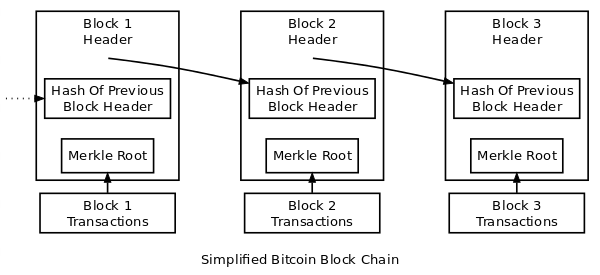
\includegraphics[width=0.8\textwidth]{./Figures/blockchain.png}
\caption{Simple Blockchain \citep{Blockchain2016}}
\label{fig:blockchain}
\end{center}
\end{figure}
The transaction data part of a block consists of one or more new transactions. While the merkel root of the merkle tree contains  hashed copies of each transaction, and the hashes are then paired, hashed, paired again, and hashed again until a single hash remains. The chaining of blocks together and storing the hash of the previous block’s header ensures a transaction cannot be modified without modifying the block that records it and all following blocks. The same goes with the transaction, which are also chained together. A single transaction can create multiple outputs, which  are tied to transaction identifiers (TXIDs), the hashes of signed transactions. Also, the outputs of all transactions included in the block chain can be categorized as either Unspent Transaction Outputs (UTXOs) or spent transaction outputs \ref{fig:block_t}. The first one of these transactions called a generation transaction, which should collect and spend the block reward (comprised of a block subsidy and any transaction fees paid by transactions included in this block). All these transactions are encoded into blocks in binary rawtransaction format, making it difficult for researchers to extract in simple relational database format, to get transaction graph.

\begin{figure}[ht]
\begin{center}
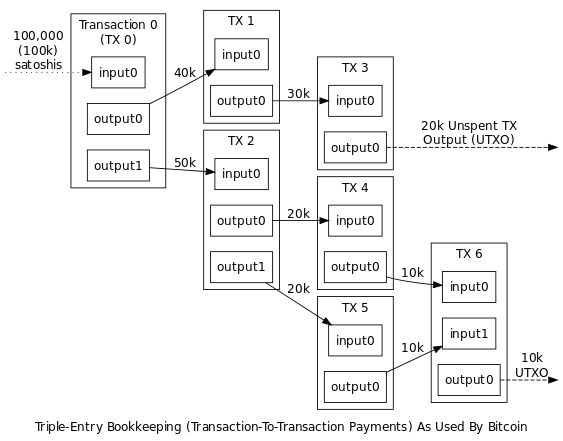
\includegraphics[width=0.8\textwidth]{./Figures/block_t.png}
\caption{Blockchain Transaction \citep{Blockchain2016}}
\label{fig:block_t}
\end{center}
\end{figure}

\section{Related Work}
The possibility to analyze agent resolved transactions in any market is limited by the scarcity of available data, as this kind of information is usually considered highly sensitive. But with the publicly available blockchain at every machine allows researchers to reconstruct the network of transactions and extract the time and amount of each payment. There are many research studies that concerns bitcoin transaction network using network analysis, machine learning and statistical physics techniques.

Parsing four (2009-2013) years data from bitcoin's  blockchain, Kondor et al. \citep{Csabai2014}  analyze the structure of the transaction network by measuring network characteristics over time, such as the degree distribution, degree correlations, clustering and money movement. Using the same data, they in their different paper \citep{Kondor2014} analyze changes in the structure of the subgraph induced by the most active users. They were  able to show find correlation between structural changes in the network and exchange price of bitcoins. But with exponential increase in the number of transaction over years, they method seems obsolete , as it is difficult to scale with their endorsed methods.

Reid and Harrigan \citep{Reid2013} linked addresses belonging to the same entity using external information. The using techniques such as context discovery and flow analysis, they investigate an alleged theft of Bitcoins. By running the Union-Find algorithm, Ron and Samir \citep{Ron2013}  associated the 3,120,948 addresses with 1,851,544 different entities to understand behaviour of users. Spagnuolo \citep{Spagnuolo2013} released open source project Bitiodine, which was able to cluster addresses and classify them using a dataset partially obtained in an automatic fashion, using scrapers for major web sources of bitcoin addresses. On the similar line, other paper \citep{Fleder2015} investigates bitcoin transaction-graph-annotation, which is capable of tracing and clustering user activity.

Most of the  previous research employed data collected from old Bitcoin- client Bitcoin 0.8 later, the newer bitcoin clients indexed the full blockchain using LevelDB instead making the publicly available bitcointools obsolete. Adding to the same, the nearing 300,000 transactions/day in 2015 gives really hard time to earlier algorithms to scale, thus motivating us to develop new techniques to parsing data from blockchain, reconstructing network and doing analysis.

\section{Data}
\label{data}
The blockchain is a transaction database of the Bitcoin.  Once Bitcoin core is setup at local machine, blockchain is automatically downloaded. Every full node participating in the Bitcoin network has the same copy. As of now there is more than 60 GB of Bitcoin blockchain dataset, which makes it difficult to parse the raw blockchain data. Most of the previous studies \citep{Ron2013} employed a forked version of bitcointools \footnote{\url{https://github.com/gavinandresen/bitcointools}}, but from the bitcoin clients 0.8 version, it indexed the full blockchain using LevelDB instead making the publicly available bitcointools obsolete. Other well know open source blockchain parser like blockparser \footnote{\url {https://github.com/znort987/blockparser}}, BitIodine \citep{Spagnuolo2013} etc are almost undocumented projects, where some appear to not even work. A paper \citep{Fleder2015} led me to BitcoinArmory project, which requires a dozen of manual interventions to get installed, but still doesn’t work.

We then started to look for ready-made SQL database, which pointed to BitcoinABe. This python based library reads the Bitcoin block file, transforms and loads the data into a SQL database \ref{fig:SQL}. But, Its takes more than two weeks to dump the data, which was not feasible option. We downloaded postgres database dumps of the bitcoin-ruby-blockchain database generated by webbtc \footnote{\url{http://dumps.webbtc.com/bitcoin/}}. Then, with slight modification to open repository BitIodine \citep{Spagnuolo2013} code, we parsed through the blockchain, and wrote wrapper classes that extracted the relevant information required to construct the transaction graph. The market price data was scarped from website \url {https://blockchain.info/} to plot graphs in R.

\section{Bitcoin Transaction Network}

Before getting the transaction network, we first define our graph, which acts as input to further mathematical application.

\begin{definition}
We consider weighted labelled graph. That is, a
graph $G=(V,E,\ell)$ is represented by a set of $|V|=n$ vertices, a
set of edges $E$ specified by a weighted adjacency matrix $A \in
\bb{R}^{n \times n}$, and a label function $\ell\colon V \rightarrow
\cm{L}$ with $\cm{L} = \left( [k], \R^D \right)$, where $k$ is the
number of available node labels and $D$ is the dimension of the
continuous attributes.  Given $V = \{v_1,v_2,...,v_n\}$, \emph{node
  labels} $\ell(v_i)$ are represented by nominal values and
\emph{attributes} $\mathbf{x}_i \in \bb R^D$ are represented by
continuous vectors. In a transaction graph, addresses are nodes, transactions are edges and weight is BTC.
\label{def:graph}
\end{definition}

With the overall transactions records parsed from the blockchain in human readable form, we construct a a weighted directed transaction graph that gives an intuition towards the flow of Bitcoins from one key to the other,the directed edge represents a particular transaction from a source address to a target address and weight represents the value of the transactions. For our experiments, we constructed graphs for more than two years (March, 2013 to December, 2015) to capture major bubble in Bitcoin history. Figure \ref{fig:dt} represent daily transaction graph for a typical day on April 8, 2013.

\begin{figure}[ht]
\begin{center}
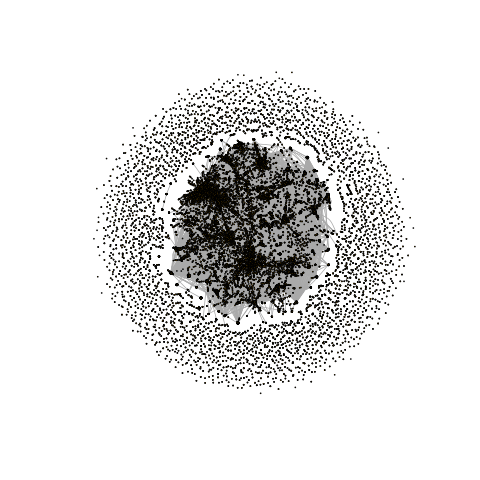
\includegraphics[width=\textwidth]{./Figures/dt.png}
\caption{ Daily transaction graph for a typical day (April 8, 2013)}
\label{fig:dt}
\end{center}
\end{figure}

\section{Transaction Dynamics}
The validation of the data parsed from our tool is then checked by
reproducing the ”Mathew Effect” phenomenon from the seminal work of Kondor et al. \citep{Csabai2014} paper’s using their original matlab code, but with our own data. The authors of the above papers are curator of whole blockchain up to 2014.10.19. (326,027 blocks), which is benchmark in quality. The similar figure confirms the high quality of our data.

To capture the transaction  dynamics in the bitcoin, we analyze the dynamics of money flow on the transaction network, as discussed in the paper \citep{Csabai2014}. We try to support popular hypothesis in economics having roots in preferential attachment, called Matthew effect or the "rich get richer phenomenon". It states that the growth of the wealth of each individual is proportional to the wealth of that individual \citep{Csabai2014}.

We assume that the number of bitcoins associated with node $n$ at time $t$ is given by $b_{n}(t)$. The difference between the balance of each
address at the end and at the start of each month is calculated. Then the difference in function of the starting balances is plotted in figure \ref{fig:dynamics}. The  positive correlation between balance and the average growth indicates the "rich get richer" phenomenon in bitcoin.

\begin{figure}[ht]
\begin{center}
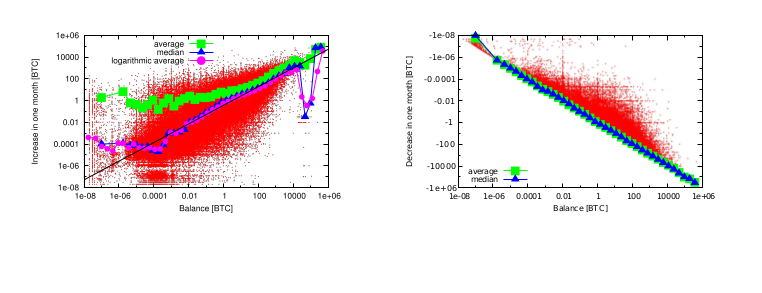
\includegraphics[width= \textwidth]{./Figures/dynamics.png}
\caption{ Matthew Effect}
\label{fig:dynamics}
\end{center}
\end{figure}

The figure \ref{fig:dynamics} is reproduced from Kondor's paper \citep{Csabai2014}, using our own data where Increase (left) and decrease (right) of node balances in one month windows as a function of their balance at the beginning of each month is represented. The representation in the picture follow the following colors: the raw data (red), the average (green), median (blue) and logarithmic average (magenta). The later three are calculated for logarithmically sized bins. The power-law fit for the double logarithmic data is represented by black line.

\subsection{Silk Road Arrest}

The Silk Road, under the alias of “Dread Pirate Roberts” (DPR) was known as an anonymous marketplace, a Black Market operated as a hidden service only accessible through Tor, where people who use bitcoins were able to buy and sell drugs, art, weapons etc. anonymously, without the risk of being tracked. It was founded by Ross William Ulbricht in February in 2011, but in October 2013 FBI closed the Silk Road and arrested Ulbricht. The FBI  seized approximately 173,600 BTC in two phase. At the first go 29,600 BTC held in a so called hot wallet were seized and an additional 144,000 BTC were seized using two addresses \footnote{1F1tAaz5x1HUXrCNLbtMDqcw6o5GNn4xqX, 1FfmbHfnpaZjKFvyi1okTjJJusN455paPH} controlled by the FBI. 

We illustrates the event using transaction network \ref{fig:silk} realised in gephi. Each vertex represents a user, where address is mapped to the user. Each directed edge between a source and a target represents a flow of Bitcoins from a public-key belonging to the user corresponding to the source to a public-key belonging to the user corresponding to the target. 

\begin{figure}[ht]
\begin{center}
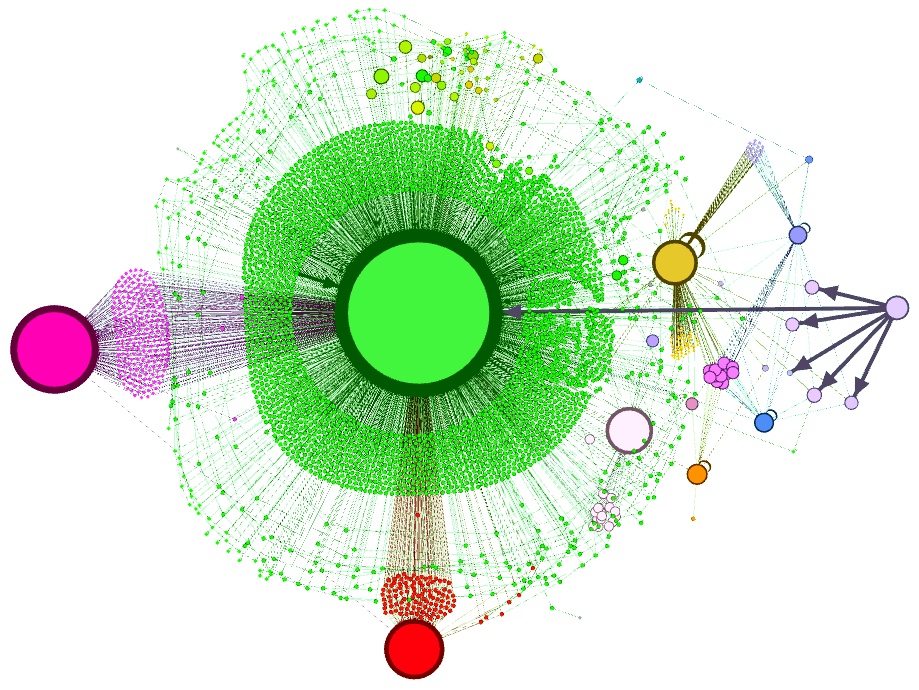
\includegraphics[width=0.7\textwidth]{./Figures/silk.png}
\caption{ Silk Road Arrest}
\label{fig:silk}
\end{center}
\end{figure}

Although in this scenario involves manual investigation by web scraping , it would have been difficult to find significant links manually, given the millions of nodes involved.

\section{Summary}
This chapter introduces Bitcoin, its working detail by explaining the protocol of blockchain, which contains all the history of transactions in the bitcoin. With enough knowledge about working of bitcoin, the related work in bitcoin transaction network is the discussed with the pros and cons. The data preparation staged is discussed to get the transaction network, an input to our mathematical model in coming chapters. The case study of silk road arrest is illustrated with the transaction graph. Transaction dynamics is reproduced from know studies to validate the parsed data, concludes the chapter. 
%----------------------------------------------------------------------------------------
%	THESIS CONTENT - CHAPTER6
%----------------------------------------------------------------------------------------

%\mainmatter % Begin numeric (1,2,3...) page numbering

\pagestyle{fancy} % Return the page headers back to the "fancy" style

% Include the chapters of the thesis as separate files from the Chapters folder
% Uncomment the lines as you write the chapters


%----------------------------------------------------------------------------------------
%	THESIS CONTENT - APPENDICES
%----------------------------------------------------------------------------------------

\addtocontents{toc}{\vspace{2em}} % Add a gap in the Contents, for aesthetics

\appendix % Cue to tell LaTeX that the following 'chapters' are Appendices

% Include the appendices of the thesis as separate files from the Appendices folder
% Uncomment the lines as you write the Appendices

% Appendix A
\chapter{Blockchain SQL Schema} % Main appendix title
\label{AppendixA} % For referencing this appendix elsewhere, use \ref{AppendixA}

\lhead{Appendix A. \emph{Blockchain SQL Schema}} % This is for the header on each page - perhaps a shortened title

\begin{figure}[ht]
\begin{center}
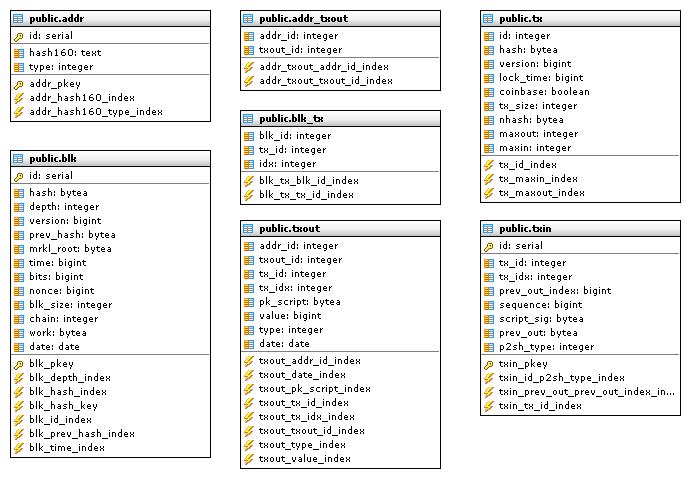
\includegraphics[width=\textwidth]{./Figures/SQL.png}
\caption{ SQL Schema of the Blockchain}
\label{fig:SQL}
\end{center}
\end{figure}

%\input{Appendices/AppendixB}
%\input{Appendices/AppendixC}

\addtocontents{toc}{\vspace{2em}} % Add a gap in the Contents, for aesthetics
%\addcontentsline{toc}{chapter}{Bibliography}
\backmatter


%----------------------------------------------------------------------------------------
%	BIBLIOGRAPHY

%----------------------------------------------------------------------------------------
\clearpage % Start a new page
\begin{thebibliography}{99}
\setlength{\parskip}{1em}

\bibitem{Lo2015} Lo, S and Wand, C. 
\newblock Bitcoin as Money?.
\newblock {\em Federal Reserve Bank of Boston, Current Policy Perspective}. 14-4, Boston.
\newblock \url {http://www.bostonfed.org/economic/current-policy-perspectives/2014/cpp1404.pdf}, 2015.

\bibitem{Kristoufek2015} Kristoufek,L.
\newblock What are the main drivers of the bitcoin price? evidence
from wavelet coherence analysis. 
\newblock {\em PLoS ONE}, 10(4), 04, 2015.

\bibitem{Donier2015} Donier, J and Bouchaud, J.
\newblock Why Do Markets Crash? Bitcoin Data Offers Unprecedented Insights.
\newblock {\em PLoS ONE}, 10(10): e0139356, 2015.

\bibitem{Ali2014}
Ali, R, Barrdear, J, Clews, J and Southgate, J.
\newblock The economics of digital currencies.
\newblock {\em Bank of England Quarterly Bulletin}, page~Q3, 2014.

\bibitem{Nakamoto2008} Nakamoto, S.
\newblock Bitcoin: A peer-to-peer electronic cash system.
\newblock {\em Consulted}, 1(2012):28, 2008.

\bibitem{Kondor2014} Kondor, D, Csabai, I, Sz{\"{u}}le, J, P{\'{o}}sfai, M and Vattay,  G.
\newblock Inferring the interplay between network structure and market
effects in bitcoin.
\newblock {\em New Journal of Physics}, 16(12):125003, 2014.

\bibitem {Zager2008} Zager, L and Verghes, G. 
\newblock Graph similarity scoring and matching. 
\newblock {\em Applied Mathematics Letters}, 21(1):86 – 94, 2008.

\bibitem{Yanardag2015} Yanardag, P and Vishwanathan, S.V.N. 
\newblock Deep graph kernels. 
\newblock {\em In Proceedings of the 21th ACM SIGKDD International Conference on Knowledge Discovery and Data Mining}, KDD ’15, pages 1365–1374, New York, USA, 2015.

\bibitem {Johannes2015} Johannes G, Keeler P, Krzesinski, A and Taylor, P. 
\newblock Bitcoin blockchain dynamics: the selfish-mine strategy in the
presence of propagation delay.
\newblock {\em CoRR, abs/1505.05343},
\newblock \url {http://arxiv.org/abs/1505.05343}, 2015.

\bibitem {Blockchain2016}
\newblock \url {https://bitcoin.org/en/developer-guide#block-chain}

\bibitem {Ron2013} Ron, D and Shamir, A.
\newblock Quantitative Analysis of the Full Bitcoin Transaction Graph.
\newblock {\em IACR Cryptology ePrint Archive}, p. 584, 2013.

\bibitem {Reid2013} Reid, F and Harrigan, M.
\newblock An Analysis of Anonymity in the Bitcoin System.
\newblock {\em Security and Privacy in Social Networks}, pp 197-223, 2013.

\bibitem {Csabai2014} Kondor, D, Csabai, I, P{\'{o}}sfai, M and Vattay,  G.
\newblock Do the Rich Get Richer? An Empirical Analysis of the Bitcoin Transaction Network. 
\newblock {\em PLOS ONE}, 9(5): e97205., 2014.

\bibitem {Spagnuolo2013} Spagnuolo, M. 
\newblock Bitiodine: Extracting intelligence from the bitcoin network. 
\newblock {\em Master’s thesis, Politecnico di Milano, Italy}, 2013

\bibitem {Fleder2015} Fleder, M, Kester, M and Pillai, S.
\newblock Bitcoin transaction graph analysis. 
\newblock {\em CoRR}, abs/1502.01657,
\newblock \url {http://arxiv.org/abs/1502.01657}, 2015.

\bibitem {Babai2016} Babai, L. 
\newblock  Graph isomorphism in quasipolynomial time. 
\newblock {\em CoRR}, abs/1512.03547, 
\newblock \url {http://arxiv.org/abs/1512.03547}, 2016.

\bibitem {Lee2012} Lee, J, Han, W.S, Kasperovics, R and Lee, J.H.
\newblock  An in-depth comparison of subgraph isomorphism algorithms in graph databases. 
\newblock {\em VLDB}, pages 133–144, 2012.

\bibitem {Gao2010} Gao,X, Xiao, B, Tao, D and Li, X.
\newblock A survey of graph edit distance.
\newblock {\em Pattern Analysis and Applications}, Volume 13, Issue 1, pp 113-129, 2010.

\bibitem {Lerouge2016} Lerouge, L, Abu{-}Aisheh, Z, Raveaux, R, H{\'{e}}roux, P and Adam, S.
\newblock Graph edit distance : a new binary linear programming formulation.
\newblock {\em CoRR}, abs/1505.05740, 
\newblock \url {http://arxiv.org/abs/1505.05740}, 2016.

\bibitem {Koutra2015} Koutra,D, Vogelstein, J.T, and Faloutsos, C.
\newblock  DELTACON: A principled massive-graph similarity function. 
\newblock {\em CoRR}, abs/1304.4657,
\newblock \url {http://arxiv.org/abs/1304.4657}, 2015.


\bibitem {Li2012} Li, G, Semerci, M, Yener, M and Zaki, M.J. 
\newblock Effective graph classification based on topological and label attributes.
\newblock {\em Stat. Anal. Data Min.}, 5(4):265–283, August 2012.

\bibitem {Mheich2015} Mheich, A, Hassan, M, Gripon,V,  Khalil, M,  Berrou, C, Dufor, O and Wendling, F.
\newblock  A novel algorithm for measuring graph similarity:
Application to brain networks. 
\newblock {\em In Neural Engineering (NER), 2015 7th
International IEEE/EMBS Conference on}, pages 1068–1071, April 2015.

\bibitem {Melnik2002} Melnik, S,  Molina, H.G, and Rahm, E.
\newblock Similarity flooding: A versatile graph matching algorithm and its application to schema matching. 
\newblock {\em In Proceedings of the 18th International Conference on Data
Engineering, ICDE ’02,}, IEEE Computer Society, pages 117–, Washington, DC, USA, 2002. 

\bibitem {Lee2015} Lee, J, Kim, G and Yoon, S.
\newblock Measuring large-scale dynamic graph similarity by ricom: RWR with intergraph compression. 
\newblock {\em In 2015 IEEE International Conference on Data Mining, ICDM 2015}, Atlantic City, NJ, USA, November 14-17, 2015, pages 829–834, 2015.


\bibitem {Haussler1999} Haussler, D. 
\newblock Convolution kernels on discrete structures.
\newblock {\em Technical Report}, UCS-CRL-99-10, University of California at Santa Cruz, Santa Cruz, CA, USA, 1999.

\bibitem {Bai2015} Bai, l, Zhang, Z,  Wang, C,  Bai, X and Hancock, E.R.
\newblock A graph kernel based on the Jensen-Shannon representation alignment. 
\newblock {\em In Proceedings of the 24th International Conference on Artificial Intelligence (IJCAI'15)}, Qiang Yang and Michael Wooldridge (Eds.). AAAI Press 3322-3328, 2015.


\bibitem {Aziz2013} Aziz,F, Wilson, R.C. and Hancock, E.R.
\newblock Backtrackless walks on a graph.
\newblock {\em Neural Networks and Learning Systems, IEEE Transactions on}, 24(6):977–989, June, 2013.

\bibitem {Vishwanathan2010} Vishwanathan, S.V.N, Schraudolph, N.N, Kondor, R and Borgwardt, K.M.
\newblock Graph kernels. 
\newblock {\em J. Mach. Learn. Res.}, 11:1201–1242, August, 2010.


\bibitem {Neumann2015} Neumann, M,  Garnett, R,  Bauckhage, C and Kersting, K. \newblock Propagation kernels: efficient graph kernels from propagated
information. 
\newblock {\em Machine Learning}, 102(2):209–245, 2015.

\bibitem {Gartner2003} G{\"a}rtner, T, Flach, P and Wrobel, S. 
\newblock On graph kernels: Hardness results and efficient alternatives.
\newblock In Sch {\"o}lkopf, B and Warmuth, M.K. editors,
\newblock {\em Proceedings of the Annual Conference on Computational Learning Theory}, pages 129–143. Springer, 2003.

\bibitem {Borgwardt2005} Borgwardt, K.M, Ong, C.S,   Sch {\"o}nauer, S, Vishwanathan, S. V. N, Smola, A.J, and Kriegel, H.P.
\newblock Protein function prediction via graph kernels.
\newblock {\em In Proceedings of Intelligent Systems in Molecular Biology (ISMB)}, Detroit, USA, 2005.


\bibitem {Kashima2003} Kashima, H,  Tsuda, K and Inokuchi, A. 
\newblock Marginalized kernels between labeled graphs. 
\newblock {\em In Proceedings of the Twentieth International Conference on Machine Learning}, pages 321–328. AAAI Press, 2003.

\bibitem {Kang2012} Kang, U, Tong, H and Sun, J.
\newblock Fast Random Walk Graph Kernel.
\newblock {\em SIAM International Conference on Data Mining (SDM)}, Anaheim, California, USA, 2012.

\bibitem {Mahe2004} Mah{\' e}, P,  Ueda, N, Akutsu, T, Perret, J.L, and  Vert, J.P. \newblock Extensions of marginalized graph kernels. 
\newblock {\em In Proceedings of the Twenty-first International Conference on Machine Learning, ICML ’04}, pages 70–, New York, NY, USA, 2004.

\bibitem {Sugiyama2015} Sugiyama, M and Borgwardt, K. 
\newblock Halting in random walk kernels.
\newblock {\em In Advances in Neural Information Processing Systems},pages 1630–1638. Curran Associates, Inc., 2015.


\bibitem {Kriegel2005}  Kriegel, H.P and Borgwardt, K.M.
\newblock  Shortest-Path Kernels on Graphs. 
\newblock {\em In Proceedings of the Fifth IEEE International Conference on Data Mining (ICDM '05)},. IEEE Computer Society, Washington, DC, USA, 74-81, 2005.

\bibitem {Martino2012}  Martino, G.D.S,  Navarin, N and  Sperduti, A.
\newblock A Tree-Based Kernel for Graphs.
\newblock {\em Proceedings of the 2012 SIAM International Conference on Data Mining}, pp 12-24, 2012.

\bibitem {Feragen2013} Feragen, A, Kasenburg, N, Petersen, J, Bruijne, D. M and Borgwardt, K.
\newblock Scalable kernels for graphs with continuous attributes.
\newblock {\em Advances in Neural Information Processing Systems 26}, page 216--224, Curran Associates, Inc., 2013.

\bibitem {Yanardag2015B} Yanardag, P and Vishwanathan, S. V. N. 
\newblock A Structural Smoothing Framework For Robust Graph Comparison. \newblock {\em NIPS 2015}, 2134-2142, 2015.

\bibitem {Kondor2016} Kondor, R and Pan, H.
\newblock The Multiscale Laplacian Graph Kernel.
\newblock {\em CoRR}, arXiv:1603.06186 
\newblock \url {http://arxiv.org/pdf/1603.06186v1.pdf}, 2016.

\bibitem {Perozzi2014} Perozzi, B,  Al-Rfou, R and Skiena, S.
\newblock DeepWalk: online learning of social representations. 
\newblock {\em In Proceedings of the 20th ACM SIGKDD international conference on Knowledge discovery and data mining (KDD '14)}, ACM, New York, NY, USA, 701-710, 2014.

\bibitem {Kandola2003} Kandola, J, Graepel,T and Taylor, J.S.
\newblock  Reducing kernel matrix diagonal dominance using semi-definite
programming. 
\newblock {\em In Proc. Annual Conf. Computational Learning
Theory, volume 2777 of Lecture Notes in Computer Science}, pages 288–302, Washington, DC, 2003.

\bibitem {Milkov2013} Mikolov, T, Sutskever, I, Chen, K, Corrado, G.S, and Dean, J. \newblock Distributed representations of words and phrases and their compositionality. 
\newblock {\em In Advances in neural information processing systems}, pp. 3111–3119, 2013.


\end{thebibliography}

\label{Bibliography}

\lhead{\emph{Bibliography}} % Change the page header to say "Bibliography"

\bibliographystyle{unsrtnat} % Use the "unsrtnat" BibTeX style for formatting the Bibliography
\addtocontents{toc}{\vspace{2em}}
%\bibliography{Bibliography} % The references (bibliography) information are stored in the file named "Bibliography.bib"

\end{document}  